\documentclass[11pt,compress,t,notes=noshow, xcolor=table]{beamer}
\usepackage[]{graphicx}
% graphicx is loaded via lmu-lecture.sty as well
\usepackage[]{color}
% maxwidth is the original width if it is less than linewidth
% otherwise use linewidth (to make sure the graphics do not exceed the margin)
\makeatletter
\def\maxwidth{ %
  \ifdim\Gin@nat@width>\linewidth
    \linewidth
  \else
    \Gin@nat@width
  \fi
}
\makeatother

% ---------------------------------%
% latex-math dependencies, do not remove:
% - mathtools
% - bm
% - siunitx
% - dsfont
% - xspace
% ---------------------------------%

%--------------------------------------------------------%
%       Language, encoding, typography
%--------------------------------------------------------%

\usepackage[english]{babel}
\usepackage[utf8]{inputenc} % Enables inputting UTF-8 symbols
% Standard AMS suite (loaded via lmu-lecture.sty)
\usepackage{amsmath,amsfonts,amssymb}

% Font for double-stroke / blackboard letters for sets of numbers (N, R, ...)
% Distribution name is "doublestroke"
% According to https://mirror.physik.tu-berlin.de/pub/CTAN/fonts/doublestroke/dsdoc.pdf
% the "bbm" package does a similar thing and may be superfluous.
% Required for latex-math
\usepackage{dsfont}

% bbm – "Blackboard-style" cm fonts (https://www.ctan.org/pkg/bbm)
% Used to be in common.tex, loaded directly after this file
% Maybe superfluous given dsfont is loaded
% TODO: Check if really unused?
% \usepackage{bbm}

% bm – Access bold symbols in maths mode - https://ctan.org/pkg/bm
% Required for latex-math, preferred over \boldsymbol
% https://tex.stackexchange.com/questions/3238/bm-package-versus-boldsymbol
\usepackage{bm}

% pifont – Access to PostScript standard Symbol and Dingbats fonts
% Used for \newcommand{\xmark}{\ding{55}, which is never used
% aside from lecture_advml/attic/xx-automl/slides.Rnw
% \usepackage{pifont}

% Quotes (inline and display), provdes \enquote
% https://ctan.org/pkg/csquotes
\usepackage{csquotes}

% Adds arg to enumerate env, technically superseded by enumitem according
% to https://ctan.org/pkg/enumerate
% Replace with https://ctan.org/pkg/enumitem ?
% Even better: enumitem is not really compatible with beamer and breaks all sorts of things
% particularly the enumerate environment. The enumerate package also just isn't required
% from what I can tell so... don't re-add it I guess?
% \usepackage{enumerate}

% Line spacing - provides \singlespacing \doublespacing \onehalfspacing
% https://ctan.org/pkg/setspace
% \usepackage{setspace}

% mathtools – Mathematical tools to use with amsmath
% https://ctan.org/pkg/mathtools?lang=en
% latex-math dependency according to latex-math repo
\usepackage{mathtools}

% Maybe not great to use this https://tex.stackexchange.com/a/197/19093
% Use align instead -- TODO: Global search & replace to check, eqnarray is used a lot
% $ rg -f -u "\begin{eqnarray" -l | grep -v attic | awk -F '/' '{print $1}' | sort | uniq -c
%   13 lecture_advml
%   14 lecture_i2ml
%    2 lecture_iml
%   27 lecture_optimization
%   45 lecture_sl
\usepackage{eqnarray}

% For shaded regions / boxes
% Used sometimes in optim
% https://www.ctan.org/pkg/framed
\usepackage{framed}

%--------------------------------------------------------%
%       Cite button (version 2024-05)
%--------------------------------------------------------%
% Note this requires biber to be in $PATH when running,
% telltale error in log would be e.g. Package biblatex Info: ... file 'authoryear.dbx' not found
% aside from obvious "biber: command not found" or similar.
% Tried moving this to lmu-lecture.sty but had issues I didn't quite understood,
% so it's here for now.

\usepackage{textcase} % for \NoCaseChange
\usepackage{hyperref}

% Only try adding a references file if it exists, otherwise
% this would compile error when references.bib is not found
\IfFileExists{references.bib} {
  \usepackage{usebib}
  \usepackage[backend=biber, style=authoryear]{biblatex}

  \addbibresource{./references.bib}
  \bibinput{references}
}

\newcommand{\citelink}[1]{%
\NoCaseChange{\resizebox{!}{9pt}{\protect\beamergotobutton{\href{\usebibentry{\NoCaseChange{#1}}{url}}{\begin{NoHyper}\cite{#1}\end{NoHyper}}}}}%
}

%--------------------------------------------------------%
%       Displaying code and algorithms
%--------------------------------------------------------%

% Reimplements verbatim environments: https://ctan.org/pkg/verbatim
% verbatim used sed at least once in
% supervised-classification/slides-classification-tasks.tex
% Removed since code should not be put on slides anyway
% \usepackage{verbatim}

% Both used together for algorithm typesetting, see also overleaf: https://www.overleaf.com/learn/latex/Algorithms
% algorithmic env is also used, but part of the bundle:
%   "algpseudocode is part of the algorithmicx bundle, it gives you an improved version of algorithmic besides providing some other features"
% According to https://tex.stackexchange.com/questions/229355/algorithm-algorithmic-algorithmicx-algorithm2e-algpseudocode-confused
\usepackage{algorithm}
\usepackage{algpseudocode}

%--------------------------------------------------------%
%       Tables
%--------------------------------------------------------%

% multi-row table cells: https://www.namsu.de/Extra/pakete/Multirow.html
% Provides \multirow
% Used e.g. in evaluation/slides-evaluation-measures-classification.tex
\usepackage{multirow}

% colortbl: https://ctan.org/pkg/colortbl
% "The package allows rows and columns to be coloured, and even individual cells." well.
% Provides \columncolor and \rowcolor
% \rowcolor is used multiple times, e.g. in knn/slides-knn.tex
\usepackage{colortbl}

% long/multi-page tables: https://texdoc.org/serve/longtable.pdf/0
% Not used in slides
% \usepackage{longtable}

% pretty table env: https://ctan.org/pkg/booktabs
% Is used
% Defines \toprule
\usepackage{booktabs}

%--------------------------------------------------------%
%       Figures: Creating, placing, verbing
%--------------------------------------------------------%

% wrapfig - Wrapping text around figures https://de.overleaf.com/learn/latex/Wrapping_text_around_figures
% Provides wrapfigure environment -used in lecture_optimization
\usepackage{wrapfig}

% Sub figures in figures and tables
% https://ctan.org/pkg/subfig -- supersedes subfigure package
% Provides \subfigure
% \subfigure not used in slides but slides-tuning-practical.pdf errors without this pkg, error due to \captionsetup undefined
\usepackage{subfig}

% Actually it's pronounced PGF https://en.wikibooks.org/wiki/LaTeX/PGF/TikZ
\usepackage{tikz}

% No idea what/why these settings are what they are but I assume they're there on purpose
\usetikzlibrary{shapes,arrows,automata,positioning,calc,chains,trees, shadows}
\tikzset{
  %Define standard arrow tip
  >=stealth',
  %Define style for boxes
  punkt/.style={
    rectangle,
    rounded corners,
    draw=black, very thick,
    text width=6.5em,
    minimum height=2em,
    text centered},
  % Define arrow style
  pil/.style={
    ->,
    thick,
    shorten <=2pt,
    shorten >=2pt,}
}

%--------------------------------------------------------%
%       Beamer setup and custom macros & environments
%--------------------------------------------------------%

% Main sty file for beamer setup (layout, style, lecture page numbering, etc.)
% For long-term maintenance, this may me refactored into a more modular set of .sty files
\usepackage{../../style/lmu-lecture}
% Custom itemize wrappers, itemizeS, itemizeL, etc
\usepackage{../../style/customitemize}
% Custom framei environment, uses custom itemize!
\usepackage{../../style/framei} 
% Column layout macros
\usepackage{../../style/splitV} 

% Used regularly
\let\code=\texttt

% Not sure what/why this does
\setkeys{Gin}{width=0.9\textwidth}

% -- knitr leftovers --
% Used often in conjunction with \definecolor{shadecolor}{rgb}{0.969, 0.969, 0.969}
% Removing definitions requires chaning _many many_ slides, which then need checking to see if output still ok
\definecolor{fgcolor}{rgb}{0.345, 0.345, 0.345}
\definecolor{shadecolor}{rgb}{0.969, 0.969, 0.969}
\newenvironment{knitrout}{}{} % an empty environment to be redefined in TeX

%-------------------------------------------------------------------------------------------------------%
%  Unused stuff that needs to go but is kept here currently juuuust in case it was important after all  %
%-------------------------------------------------------------------------------------------------------%

% \newcommand{\hlnum}[1]{\textcolor[rgb]{0.686,0.059,0.569}{#1}}%
% \newcommand{\hlstr}[1]{\textcolor[rgb]{0.192,0.494,0.8}{#1}}%
% \newcommand{\hlcom}[1]{\textcolor[rgb]{0.678,0.584,0.686}{\textit{#1}}}%
% \newcommand{\hlopt}[1]{\textcolor[rgb]{0,0,0}{#1}}%
% \newcommand{\hlstd}[1]{\textcolor[rgb]{0.345,0.345,0.345}{#1}}%
% \newcommand{\hlkwa}[1]{\textcolor[rgb]{0.161,0.373,0.58}{\textbf{#1}}}%
% \newcommand{\hlkwb}[1]{\textcolor[rgb]{0.69,0.353,0.396}{#1}}%
% \newcommand{\hlkwc}[1]{\textcolor[rgb]{0.333,0.667,0.333}{#1}}%
% \newcommand{\hlkwd}[1]{\textcolor[rgb]{0.737,0.353,0.396}{\textbf{#1}}}%
% \let\hlipl\hlkwb

% \makeatletter
% \newenvironment{kframe}{%
%  \def\at@end@of@kframe{}%
%  \ifinner\ifhmode%
%   \def\at@end@of@kframe{\end{minipage}}%
%   \begin{minipage}{\columnwidth}%
%  \fi\fi%
%  \def\FrameCommand##1{\hskip\@totalleftmargin \hskip-\fboxsep
%  \colorbox{shadecolor}{##1}\hskip-\fboxsep
%      % There is no \\@totalrightmargin, so:
%      \hskip-\linewidth \hskip-\@totalleftmargin \hskip\columnwidth}%
%  \MakeFramed {\advance\hsize-\width
%    \@totalleftmargin\z@ \linewidth\hsize
%    \@setminipage}}%
%  {\par\unskip\endMakeFramed%
%  \at@end@of@kframe}
% \makeatother

% \definecolor{shadecolor}{rgb}{.97, .97, .97}
% \definecolor{messagecolor}{rgb}{0, 0, 0}
% \definecolor{warningcolor}{rgb}{1, 0, 1}
% \definecolor{errorcolor}{rgb}{1, 0, 0}
% \newenvironment{knitrout}{}{} % an empty environment to be redefined in TeX

% \usepackage{alltt}
% \newcommand{\SweaveOpts}[1]{}  % do not interfere with LaTeX
% \newcommand{\SweaveInput}[1]{} % because they are not real TeX commands
% \newcommand{\Sexpr}[1]{}       % will only be parsed by R
% \newcommand{\xmark}{\ding{55}}%

% textpos – Place boxes at arbitrary positions on the LATEX page
% https://ctan.org/pkg/textpos
% Provides \begin{textblock}
% TODO: Check if really unused?
% \usepackage[absolute,overlay]{textpos}

% -----------------------%
% Likely knitr leftovers %
% -----------------------%

% psfrag – Replace strings in encapsulated PostScript figures
% https://www.overleaf.com/latex/examples/psfrag-example/tggxhgzwrzhn
% https://ftp.mpi-inf.mpg.de/pub/tex/mirror/ftp.dante.de/pub/tex/macros/latex/contrib/psfrag/pfgguide.pdf
% Can't tell if this is needed
% TODO: Check if really unused?
% \usepackage{psfrag}

% arydshln – Draw dash-lines in array/tabular
% https://www.ctan.org/pkg/arydshln
% !! "arydshln has to be loaded after array, longtable, colortab and/or colortbl"
% Provides \hdashline and \cdashline
% Not used in slides
% \usepackage{arydshln}

% tabularx – Tabulars with adjustable-width columns
% https://ctan.org/pkg/tabularx
% Provides \begin{tabularx}
% Not used in slides
% \usepackage{tabularx}

% placeins – Control float placement
% https://ctan.org/pkg/placeins
% Defines a \FloatBarrier command
% TODO: Check if really unused?
% \usepackage{placeins}

% Can't find a reason why common.tex is not just part of this file?
% This file is included in slides and exercises

% Rarely used fontstyle for R packages, used only in 
% - forests/slides-forests-benchmark.tex
% - exercises/single-exercises/methods_l_1.Rnw
% - slides/cart/attic/slides_extra_trees.Rnw
\newcommand{\pkg}[1]{{\fontseries{b}\selectfont #1}}

% Spacing helpers, used often (mostly in exercises for \dlz)
\newcommand{\lz}{\vspace{0.5cm}} % vertical space (used often in slides)
\newcommand{\dlz}{\vspace{1cm}}  % double vertical space (used often in exercises, never in slides)
\newcommand{\oneliner}[1] % Oneliner for important statements, used e.g. in iml, algods
{\begin{block}{}\begin{center}\begin{Large}#1\end{Large}\end{center}\end{block}}

% Don't know if this is used or needed, remove?
% textcolor that works in mathmode
% https://tex.stackexchange.com/a/261480
% Used e.g. in forests/slides-forests-bagging.tex
% [...] \textcolor{blue}{\tfrac{1}{M}\sum^M_{m} [...]
% \makeatletter
% \renewcommand*{\@textcolor}[3]{%
%   \protect\leavevmode
%   \begingroup
%     \color#1{#2}#3%
%   \endgroup
% }
% \makeatother


% math spaces
\ifdefined\N                                                                
\renewcommand{\N}{\mathds{N}} % N, naturals
\else \newcommand{\N}{\mathds{N}} \fi 
\newcommand{\Z}{\mathds{Z}} % Z, integers
\newcommand{\Q}{\mathds{Q}} % Q, rationals
\newcommand{\R}{\mathds{R}} % R, reals
\ifdefined\C 
  \renewcommand{\C}{\mathds{C}} % C, complex
\else \newcommand{\C}{\mathds{C}} \fi
\newcommand{\continuous}{\mathcal{C}} % C, space of continuous functions
\newcommand{\M}{\mathcal{M}} % machine numbers
\newcommand{\epsm}{\epsilon_m} % maximum error

% counting / finite sets
\newcommand{\setzo}{\{0, 1\}} % set 0, 1
\newcommand{\setmp}{\{-1, +1\}} % set -1, 1
\newcommand{\unitint}{[0, 1]} % unit interval

% basic math stuff
\newcommand{\xt}{\tilde x} % x tilde
\newcommand{\argmax}{\operatorname{arg\,max}} % argmax
\newcommand{\argmin}{\operatorname{arg\,min}} % argmin
\newcommand{\argminlim}{\mathop{\mathrm{arg\,min}}\limits} % argmax with limits
\newcommand{\argmaxlim}{\mathop{\mathrm{arg\,max}}\limits} % argmin with limits  
\newcommand{\sign}{\operatorname{sign}} % sign, signum
\newcommand{\I}{\mathbb{I}} % I, indicator
\newcommand{\order}{\mathcal{O}} % O, order
\newcommand{\pd}[2]{\frac{\partial{#1}}{\partial #2}} % partial derivative
\newcommand{\floorlr}[1]{\left\lfloor #1 \right\rfloor} % floor
\newcommand{\ceillr}[1]{\left\lceil #1 \right\rceil} % ceiling

% sums and products
\newcommand{\sumin}{\sum\limits_{i=1}^n} % summation from i=1 to n
\newcommand{\sumim}{\sum\limits_{i=1}^m} % summation from i=1 to m
\newcommand{\sumjn}{\sum\limits_{j=1}^n} % summation from j=1 to p
\newcommand{\sumjp}{\sum\limits_{j=1}^p} % summation from j=1 to p
\newcommand{\sumik}{\sum\limits_{i=1}^k} % summation from i=1 to k
\newcommand{\sumkg}{\sum\limits_{k=1}^g} % summation from k=1 to g
\newcommand{\sumjg}{\sum\limits_{j=1}^g} % summation from j=1 to g
\newcommand{\meanin}{\frac{1}{n} \sum\limits_{i=1}^n} % mean from i=1 to n
\newcommand{\meanim}{\frac{1}{m} \sum\limits_{i=1}^m} % mean from i=1 to n
\newcommand{\meankg}{\frac{1}{g} \sum\limits_{k=1}^g} % mean from k=1 to g
\newcommand{\prodin}{\prod\limits_{i=1}^n} % product from i=1 to n
\newcommand{\prodkg}{\prod\limits_{k=1}^g} % product from k=1 to g
\newcommand{\prodjp}{\prod\limits_{j=1}^p} % product from j=1 to p

% linear algebra
\newcommand{\one}{\boldsymbol{1}} % 1, unitvector
\newcommand{\zero}{\mathbf{0}} % 0-vector
\newcommand{\id}{\boldsymbol{I}} % I, identity
\newcommand{\diag}{\operatorname{diag}} % diag, diagonal
\newcommand{\trace}{\operatorname{tr}} % tr, trace
\newcommand{\spn}{\operatorname{span}} % span
\newcommand{\scp}[2]{\left\langle #1, #2 \right\rangle} % <.,.>, scalarproduct
\newcommand{\mat}[1]{\begin{pmatrix} #1 \end{pmatrix}} % short pmatrix command
\newcommand{\Amat}{\mathbf{A}} % matrix A
\newcommand{\Deltab}{\mathbf{\Delta}} % error term for vectors

% basic probability + stats
\renewcommand{\P}{\mathds{P}} % P, probability
\newcommand{\E}{\mathds{E}} % E, expectation
\newcommand{\var}{\mathsf{Var}} % Var, variance
\newcommand{\cov}{\mathsf{Cov}} % Cov, covariance
\newcommand{\corr}{\mathsf{Corr}} % Corr, correlation
\newcommand{\normal}{\mathcal{N}} % N of the normal distribution
\newcommand{\iid}{\overset{i.i.d}{\sim}} % dist with i.i.d superscript
\newcommand{\distas}[1]{\overset{#1}{\sim}} % ... is distributed as ...

% machine learning
\newcommand{\Xspace}{\mathcal{X}} % X, input space
\newcommand{\Yspace}{\mathcal{Y}} % Y, output space
\newcommand{\nset}{\{1, \ldots, n\}} % set from 1 to n
\newcommand{\pset}{\{1, \ldots, p\}} % set from 1 to p
\newcommand{\gset}{\{1, \ldots, g\}} % set from 1 to g
\newcommand{\Pxy}{\mathbb{P}_{xy}} % P_xy
\newcommand{\Exy}{\mathbb{E}_{xy}} % E_xy: Expectation over random variables xy
\newcommand{\xv}{\mathbf{x}} % vector x (bold)
\newcommand{\xtil}{\tilde{\mathbf{x}}} % vector x-tilde (bold)
\newcommand{\yv}{\mathbf{y}} % vector y (bold)
\newcommand{\xy}{(\xv, y)} % observation (x, y)
\newcommand{\xvec}{\left(x_1, \ldots, x_p\right)^\top} % (x1, ..., xp) 
\newcommand{\Xmat}{\mathbf{X}} % Design matrix
\newcommand{\allDatasets}{\mathds{D}} % The set of all datasets
\newcommand{\allDatasetsn}{\mathds{D}_n}  % The set of all datasets of size n 
\newcommand{\D}{\mathcal{D}} % D, data
\newcommand{\Dn}{\D_n} % D_n, data of size n
\newcommand{\Dtrain}{\mathcal{D}_{\text{train}}} % D_train, training set
\newcommand{\Dtest}{\mathcal{D}_{\text{test}}} % D_test, test set
\newcommand{\xyi}[1][i]{\left(\xv^{(#1)}, y^{(#1)}\right)} % (x^i, y^i), i-th observation
\newcommand{\Dset}{\left( \xyi[1], \ldots, \xyi[n]\right)} % {(x1,y1)), ..., (xn,yn)}, data
\newcommand{\defAllDatasetsn}{(\Xspace \times \Yspace)^n} % Def. of the set of all datasets of size n 
\newcommand{\defAllDatasets}{\bigcup_{n \in \N}(\Xspace \times \Yspace)^n} % Def. of the set of all datasets 
\newcommand{\xdat}{\left\{ \xv^{(1)}, \ldots, \xv^{(n)}\right\}} % {x1, ..., xn}, input data
\newcommand{\ydat}{\left\{ \yv^{(1)}, \ldots, \yv^{(n)}\right\}} % {y1, ..., yn}, input data
\newcommand{\yvec}{\left(y^{(1)}, \hdots, y^{(n)}\right)^\top} % (y1, ..., yn), vector of outcomes
\renewcommand{\xi}[1][i]{\xv^{(#1)}} % x^i, i-th observed value of x
\newcommand{\yi}[1][i]{y^{(#1)}} % y^i, i-th observed value of y 
\newcommand{\xivec}{\left(x^{(i)}_1, \ldots, x^{(i)}_p\right)^\top} % (x1^i, ..., xp^i), i-th observation vector
\newcommand{\xj}{\xv_j} % x_j, j-th feature
\newcommand{\xjvec}{\left(x^{(1)}_j, \ldots, x^{(n)}_j\right)^\top} % (x^1_j, ..., x^n_j), j-th feature vector
\newcommand{\phiv}{\mathbf{\phi}} % Basis transformation function phi
\newcommand{\phixi}{\mathbf{\phi}^{(i)}} % Basis transformation of xi: phi^i := phi(xi)

%%%%%% ml - models general
\newcommand{\lamv}{\bm{\lambda}} % lambda vector, hyperconfiguration vector
\newcommand{\Lam}{\bm{\Lambda}}	 % Lambda, space of all hpos
% Inducer / Inducing algorithm
\newcommand{\preimageInducer}{\left(\defAllDatasets\right)\times\Lam} % Set of all datasets times the hyperparameter space
\newcommand{\preimageInducerShort}{\allDatasets\times\Lam} % Set of all datasets times the hyperparameter space
% Inducer / Inducing algorithm
\newcommand{\ind}{\mathcal{I}} % Inducer, inducing algorithm, learning algorithm 

% continuous prediction function f
\newcommand{\ftrue}{f_{\text{true}}}  % True underlying function (if a statistical model is assumed)
\newcommand{\ftruex}{\ftrue(\xv)} % True underlying function (if a statistical model is assumed)
\newcommand{\fx}{f(\xv)} % f(x), continuous prediction function
\newcommand{\fdomains}{f: \Xspace \rightarrow \R^g} % f with domain and co-domain
\newcommand{\Hspace}{\mathcal{H}} % hypothesis space where f is from
\newcommand{\fbayes}{f^{\ast}} % Bayes-optimal model
\newcommand{\fxbayes}{f^{\ast}(\xv)} % Bayes-optimal model
\newcommand{\fkx}[1][k]{f_{#1}(\xv)} % f_j(x), discriminant component function
\newcommand{\fh}{\hat{f}} % f hat, estimated prediction function
\newcommand{\fxh}{\fh(\xv)} % fhat(x)
\newcommand{\fxt}{f(\xv ~|~ \thetab)} % f(x | theta)
\newcommand{\fxi}{f\left(\xv^{(i)}\right)} % f(x^(i))
\newcommand{\fxih}{\hat{f}\left(\xv^{(i)}\right)} % f(x^(i))
\newcommand{\fxit}{f\left(\xv^{(i)} ~|~ \thetab\right)} % f(x^(i) | theta)
\newcommand{\fhD}{\fh_{\D}} % fhat_D, estimate of f based on D
\newcommand{\fhDtrain}{\fh_{\Dtrain}} % fhat_Dtrain, estimate of f based on D
\newcommand{\fhDnlam}{\fh_{\Dn, \lamv}} %model learned on Dn with hp lambda
\newcommand{\fhDlam}{\fh_{\D, \lamv}} %model learned on D with hp lambda
\newcommand{\fhDnlams}{\fh_{\Dn, \lamv^\ast}} %model learned on Dn with optimal hp lambda 
\newcommand{\fhDlams}{\fh_{\D, \lamv^\ast}} %model learned on D with optimal hp lambda 

% discrete prediction function h
\newcommand{\hx}{h(\xv)} % h(x), discrete prediction function
\newcommand{\hh}{\hat{h}} % h hat
\newcommand{\hxh}{\hat{h}(\xv)} % hhat(x)
\newcommand{\hxt}{h(\xv | \thetab)} % h(x | theta)
\newcommand{\hxi}{h\left(\xi\right)} % h(x^(i))
\newcommand{\hxit}{h\left(\xi ~|~ \thetab\right)} % h(x^(i) | theta)
\newcommand{\hbayes}{h^{\ast}} % Bayes-optimal classification model
\newcommand{\hxbayes}{h^{\ast}(\xv)} % Bayes-optimal classification model

% yhat
\newcommand{\yh}{\hat{y}} % yhat for prediction of target
\newcommand{\yih}{\hat{y}^{(i)}} % yhat^(i) for prediction of ith targiet
\newcommand{\resi}{\yi- \yih}

% theta
\newcommand{\thetah}{\hat{\theta}} % theta hat
\newcommand{\thetab}{\bm{\theta}} % theta vector
\newcommand{\thetabh}{\bm{\hat\theta}} % theta vector hat
\newcommand{\thetat}[1][t]{\thetab^{[#1]}} % theta^[t] in optimization
\newcommand{\thetatn}[1][t]{\thetab^{[#1 +1]}} % theta^[t+1] in optimization
\newcommand{\thetahDnlam}{\thetabh_{\Dn, \lamv}} %theta learned on Dn with hp lambda
\newcommand{\thetahDlam}{\thetabh_{\D, \lamv}} %theta learned on D with hp lambda
\newcommand{\mint}{\min_{\thetab \in \Theta}} % min problem theta
\newcommand{\argmint}{\argmin_{\thetab \in \Theta}} % argmin theta

% densities + probabilities
% pdf of x 
\newcommand{\pdf}{p} % p
\newcommand{\pdfx}{p(\xv)} % p(x)
\newcommand{\pixt}{\pi(\xv~|~ \thetab)} % pi(x|theta), pdf of x given theta
\newcommand{\pixit}[1][i]{\pi\left(\xi[#1] ~|~ \thetab\right)} % pi(x^i|theta), pdf of x given theta
\newcommand{\pixii}{\pi\left(\xi\right)} % pi(x^i), pdf of i-th x 

% pdf of (x, y)
\newcommand{\pdfxy}{p(\xv,y)} % p(x, y)
\newcommand{\pdfxyt}{p(\xv, y ~|~ \thetab)} % p(x, y | theta)
\newcommand{\pdfxyit}{p\left(\xi, \yi ~|~ \thetab\right)} % p(x^(i), y^(i) | theta)

% pdf of x given y
\newcommand{\pdfxyk}[1][k]{p(\xv | y= #1)} % p(x | y = k)
\newcommand{\lpdfxyk}[1][k]{\log p(\xv | y= #1)} % log p(x | y = k)
\newcommand{\pdfxiyk}[1][k]{p\left(\xi | y= #1 \right)} % p(x^i | y = k)

% prior probabilities
\newcommand{\pik}[1][k]{\pi_{#1}} % pi_k, prior
\newcommand{\lpik}[1][k]{\log \pi_{#1}} % log pi_k, log of the prior
\newcommand{\pit}{\pi(\thetab)} % Prior probability of parameter theta

% posterior probabilities
\newcommand{\post}{\P(y = 1 ~|~ \xv)} % P(y = 1 | x), post. prob for y=1
\newcommand{\postk}[1][k]{\P(y = #1 ~|~ \xv)} % P(y = k | y), post. prob for y=k
\newcommand{\pidomains}{\pi: \Xspace \rightarrow \unitint} % pi with domain and co-domain
\newcommand{\pibayes}{\pi^{\ast}} % Bayes-optimal classification model
\newcommand{\pixbayes}{\pi^{\ast}(\xv)} % Bayes-optimal classification model
\newcommand{\pix}{\pi(\xv)} % pi(x), P(y = 1 | x)
\newcommand{\piv}{\bm{\pi}} % pi, bold, as vector
\newcommand{\pikx}[1][k]{\pi_{#1}(\xv)} % pi_k(x), P(y = k | x)
\newcommand{\pikxt}[1][k]{\pi_{#1}(\xv ~|~ \thetab)} % pi_k(x | theta), P(y = k | x, theta)
\newcommand{\pixh}{\hat \pi(\xv)} % pi(x) hat, P(y = 1 | x) hat
\newcommand{\pikxh}[1][k]{\hat \pi_{#1}(\xv)} % pi_k(x) hat, P(y = k | x) hat
\newcommand{\pixih}{\hat \pi(\xi)} % pi(x^(i)) with hat
\newcommand{\pikxih}[1][k]{\hat \pi_{#1}(\xi)} % pi_k(x^(i)) with hat
\newcommand{\pdfygxt}{p(y ~|~\xv, \thetab)} % p(y | x, theta)
\newcommand{\pdfyigxit}{p\left(\yi ~|~\xi, \thetab\right)} % p(y^i |x^i, theta)
\newcommand{\lpdfygxt}{\log \pdfygxt } % log p(y | x, theta)
\newcommand{\lpdfyigxit}{\log \pdfyigxit} % log p(y^i |x^i, theta)

% probababilistic
\newcommand{\bayesrulek}[1][k]{\frac{\P(\xv | y= #1) \P(y= #1)}{\P(\xv)}} % Bayes rule
\newcommand{\muk}{\bm{\mu_k}} % mean vector of class-k Gaussian (discr analysis) 

% residual and margin
\newcommand{\eps}{\epsilon} % residual, stochastic
\newcommand{\epsi}{\epsilon^{(i)}} % epsilon^i, residual, stochastic
\newcommand{\epsh}{\hat{\epsilon}} % residual, estimated
\newcommand{\yf}{y \fx} % y f(x), margin
\newcommand{\yfi}{\yi \fxi} % y^i f(x^i), margin
\newcommand{\Sigmah}{\hat \Sigma} % estimated covariance matrix
\newcommand{\Sigmahj}{\hat \Sigma_j} % estimated covariance matrix for the j-th class

% ml - loss, risk, likelihood
\newcommand{\Lyf}{L\left(y, f\right)} % L(y, f), loss function
\newcommand{\Lypi}{L\left(y, \pi\right)} % L(y, pi), loss function
\newcommand{\Lxy}{L\left(y, \fx\right)} % L(y, f(x)), loss function
\newcommand{\Lxyi}{L\left(\yi, \fxi\right)} % loss of observation
\newcommand{\Lxyt}{L\left(y, \fxt\right)} % loss with f parameterized
\newcommand{\Lxyit}{L\left(\yi, \fxit\right)} % loss of observation with f parameterized
\newcommand{\Lxym}{L\left(\yi, f\left(\bm{\tilde{x}}^{(i)} ~|~ \thetab\right)\right)} % loss of observation with f parameterized
\newcommand{\Lpixy}{L\left(y, \pix\right)} % loss in classification
\newcommand{\Lpiv}{L\left(y, \piv\right)} % loss in classification
\newcommand{\Lpixyi}{L\left(\yi, \pixii\right)} % loss of observation in classification
\newcommand{\Lpixyt}{L\left(y, \pixt\right)} % loss with pi parameterized
\newcommand{\Lpixyit}{L\left(\yi, \pixit\right)} % loss of observation with pi parameterized
\newcommand{\Lhxy}{L\left(y, \hx\right)} % L(y, h(x)), loss function on discrete classes
\newcommand{\Lr}{L\left(r\right)} % L(r), loss defined on residual (reg) / margin (classif)
\newcommand{\lone}{|y - \fx|} % L1 loss
\newcommand{\ltwo}{\left(y - \fx\right)^2} % L2 loss
\newcommand{\lbernoullimp}{\ln(1 + \exp(-y \cdot \fx))} % Bernoulli loss for -1, +1 encoding
\newcommand{\lbernoullizo}{- y \cdot \fx + \log(1 + \exp(\fx))} % Bernoulli loss for 0, 1 encoding
\newcommand{\lcrossent}{- y \log \left(\pix\right) - (1 - y) \log \left(1 - \pix\right)} % cross-entropy loss
\newcommand{\lbrier}{\left(\pix - y \right)^2} % Brier score
\newcommand{\risk}{\mathcal{R}} % R, risk
\newcommand{\riskbayes}{\mathcal{R}^\ast}
\newcommand{\riskf}{\risk(f)} % R(f), risk
\newcommand{\riskdef}{\E_{y|\xv}\left(\Lxy \right)} % risk def (expected loss)
\newcommand{\riskt}{\mathcal{R}(\thetab)} % R(theta), risk
\newcommand{\riske}{\mathcal{R}_{\text{emp}}} % R_emp, empirical risk w/o factor 1 / n
\newcommand{\riskeb}{\bar{\mathcal{R}}_{\text{emp}}} % R_emp, empirical risk w/ factor 1 / n
\newcommand{\riskef}{\riske(f)} % R_emp(f)
\newcommand{\risket}{\mathcal{R}_{\text{emp}}(\thetab)} % R_emp(theta)
\newcommand{\riskr}{\mathcal{R}_{\text{reg}}} % R_reg, regularized risk
\newcommand{\riskrt}{\mathcal{R}_{\text{reg}}(\thetab)} % R_reg(theta)
\newcommand{\riskrf}{\riskr(f)} % R_reg(f)
\newcommand{\riskrth}{\hat{\mathcal{R}}_{\text{reg}}(\thetab)} % hat R_reg(theta)
\newcommand{\risketh}{\hat{\mathcal{R}}_{\text{emp}}(\thetab)} % hat R_emp(theta)
\newcommand{\LL}{\mathcal{L}} % L, likelihood
\newcommand{\LLt}{\mathcal{L}(\thetab)} % L(theta), likelihood
\newcommand{\LLtx}{\mathcal{L}(\thetab | \xv)} % L(theta|x), likelihood
\newcommand{\logl}{\ell} % l, log-likelihood
\newcommand{\loglt}{\logl(\thetab)} % l(theta), log-likelihood
\newcommand{\logltx}{\logl(\thetab | \xv)} % l(theta|x), log-likelihood
\newcommand{\errtrain}{\text{err}_{\text{train}}} % training error
\newcommand{\errtest}{\text{err}_{\text{test}}} % test error
\newcommand{\errexp}{\overline{\text{err}_{\text{test}}}} % avg training error

% lm
\newcommand{\thx}{\thetab^\top \xv} % linear model
\newcommand{\olsest}{(\Xmat^\top \Xmat)^{-1} \Xmat^\top \yv} % OLS estimator in LM 

% ml - bagging, random forest
\newcommand{\bl}[1][m]{b^{[#1]}} % baselearner, default m
\newcommand{\blh}[1][m]{\hat{b}^{[#1]}} % estimated base learner, default m 
\newcommand{\blx}[1][m]{b^{[#1]}(\xv)} % baselearner, default m
\newcommand{\fM}{f^{[M]}(\xv)} % ensembled predictor
\newcommand{\fMh}{\hat f^{[M]}(\xv)} % estimated ensembled predictor
\newcommand{\ambifM}{\Delta\left(\fM\right)} % ambiguity/instability of ensemble
\newcommand{\betam}[1][m]{\beta^{[#1]}} % weight of basemodel m
\newcommand{\betamh}[1][m]{\hat{\beta}^{[#1]}} % weight of basemodel m with hat
\newcommand{\betaM}{\beta^{[M]}} % last baselearner

% ml - boosting
\newcommand{\fm}[1][m]{f^{[#1]}} % prediction in iteration m
\newcommand{\fmh}[1][m]{\hat{f}^{[#1]}} % prediction in iteration m
\newcommand{\fmd}[1][m]{f^{[#1-1]}} % prediction m-1
\newcommand{\fmdh}[1][m]{\hat{f}^{[#1-1]}} % prediction m-1
\newcommand{\errm}[1][m]{\text{err}^{[#1]}} % weighted in-sample misclassification rate
\newcommand{\wm}[1][m]{w^{[#1]}} % weight vector of basemodel m
\newcommand{\wmi}[1][m]{w^{[#1](i)}} % weight of obs i of basemodel m
\newcommand{\thetam}[1][m]{\thetab^{[#1]}} % parameters of basemodel m
\newcommand{\thetamh}[1][m]{\hat{\thetab}^{[#1]}} % parameters of basemodel m with hat
\newcommand{\blxt}[1][m]{b(\xv, \thetab^{[#1]})} % baselearner, default m
\newcommand{\ens}{\sum_{m=1}^M \betam \blxt} % ensemble
\newcommand{\rmm}[1][m]{\tilde{r}^{[#1]}} % pseudo residuals
\newcommand{\rmi}[1][m]{\tilde{r}^{[#1](i)}} % pseudo residuals
\newcommand{\Rtm}[1][m]{R_{t}^{[#1]}} % terminal-region
\newcommand{\Tm}[1][m]{T^{[#1]}} % terminal-region
\newcommand{\ctm}[1][m]{c_t^{[#1]}} % mean, terminal-regions
\newcommand{\ctmh}[1][m]{\hat{c}_t^{[#1]}} % mean, terminal-regions with hat
\newcommand{\ctmt}[1][m]{\tilde{c}_t^{[#1]}} % mean, terminal-regions
\newcommand{\Lp}{L^\prime}
\newcommand{\Ldp}{L^{\prime\prime}}
\newcommand{\Lpleft}{\Lp_{\text{left}}}
% ml - trees, extra trees

\newcommand{\Np}{\mathcal{N}} % (Parent) node N
\newcommand{\Npk}{\Np_k} % node N_k
\newcommand{\Nl}{\Np_1}	% Left node N_1
\newcommand{\Nr}{\Np_2} % Right node N_2
\newcommand{\pikN}[1][k]{\pi_#1^{(\Np)}} % class probability node N
\newcommand{\pikNh}[1][k]{\hat\pi_#1^{(\Np)}} % estimated class probability node N
\newcommand{\pikNlh}[1][k]{\hat\pi_#1^{(\Nl)}} % estimated class probability left node
\newcommand{\pikNrh}[1][k]{\hat\pi_#1^{(\Nr)}} % estimated class probability right node


\newcommand{\titlefigure}{figure/compboost-illustration-2.png}
\newcommand{\learninggoals}{
  \item Details of nonlinear BLs and splines
  \item Understand the built-in feature selection process
  \item Fair base learner selection
  \item Feature importance and PDPs
}

\title{Introduction to Machine Learning}
\date{}

\begin{document}

\lecturechapter{Componentwise Gradient Boosting}
\lecture{Introduction to Machine Learning}

% ------------------------------------------------------------------------------

\begin{vbframe}{Nonlinear base learners}

As an alternative we can use nonlinear base learners, such as $P$- or
$B$-splines, which make the model equivalent to a
\textbf{generalized additive model (GAM)} (as long as the base learners keep
their additive structure, which is the case for splines).
\vspace{0.5cm}

\vfill

\begin{center}
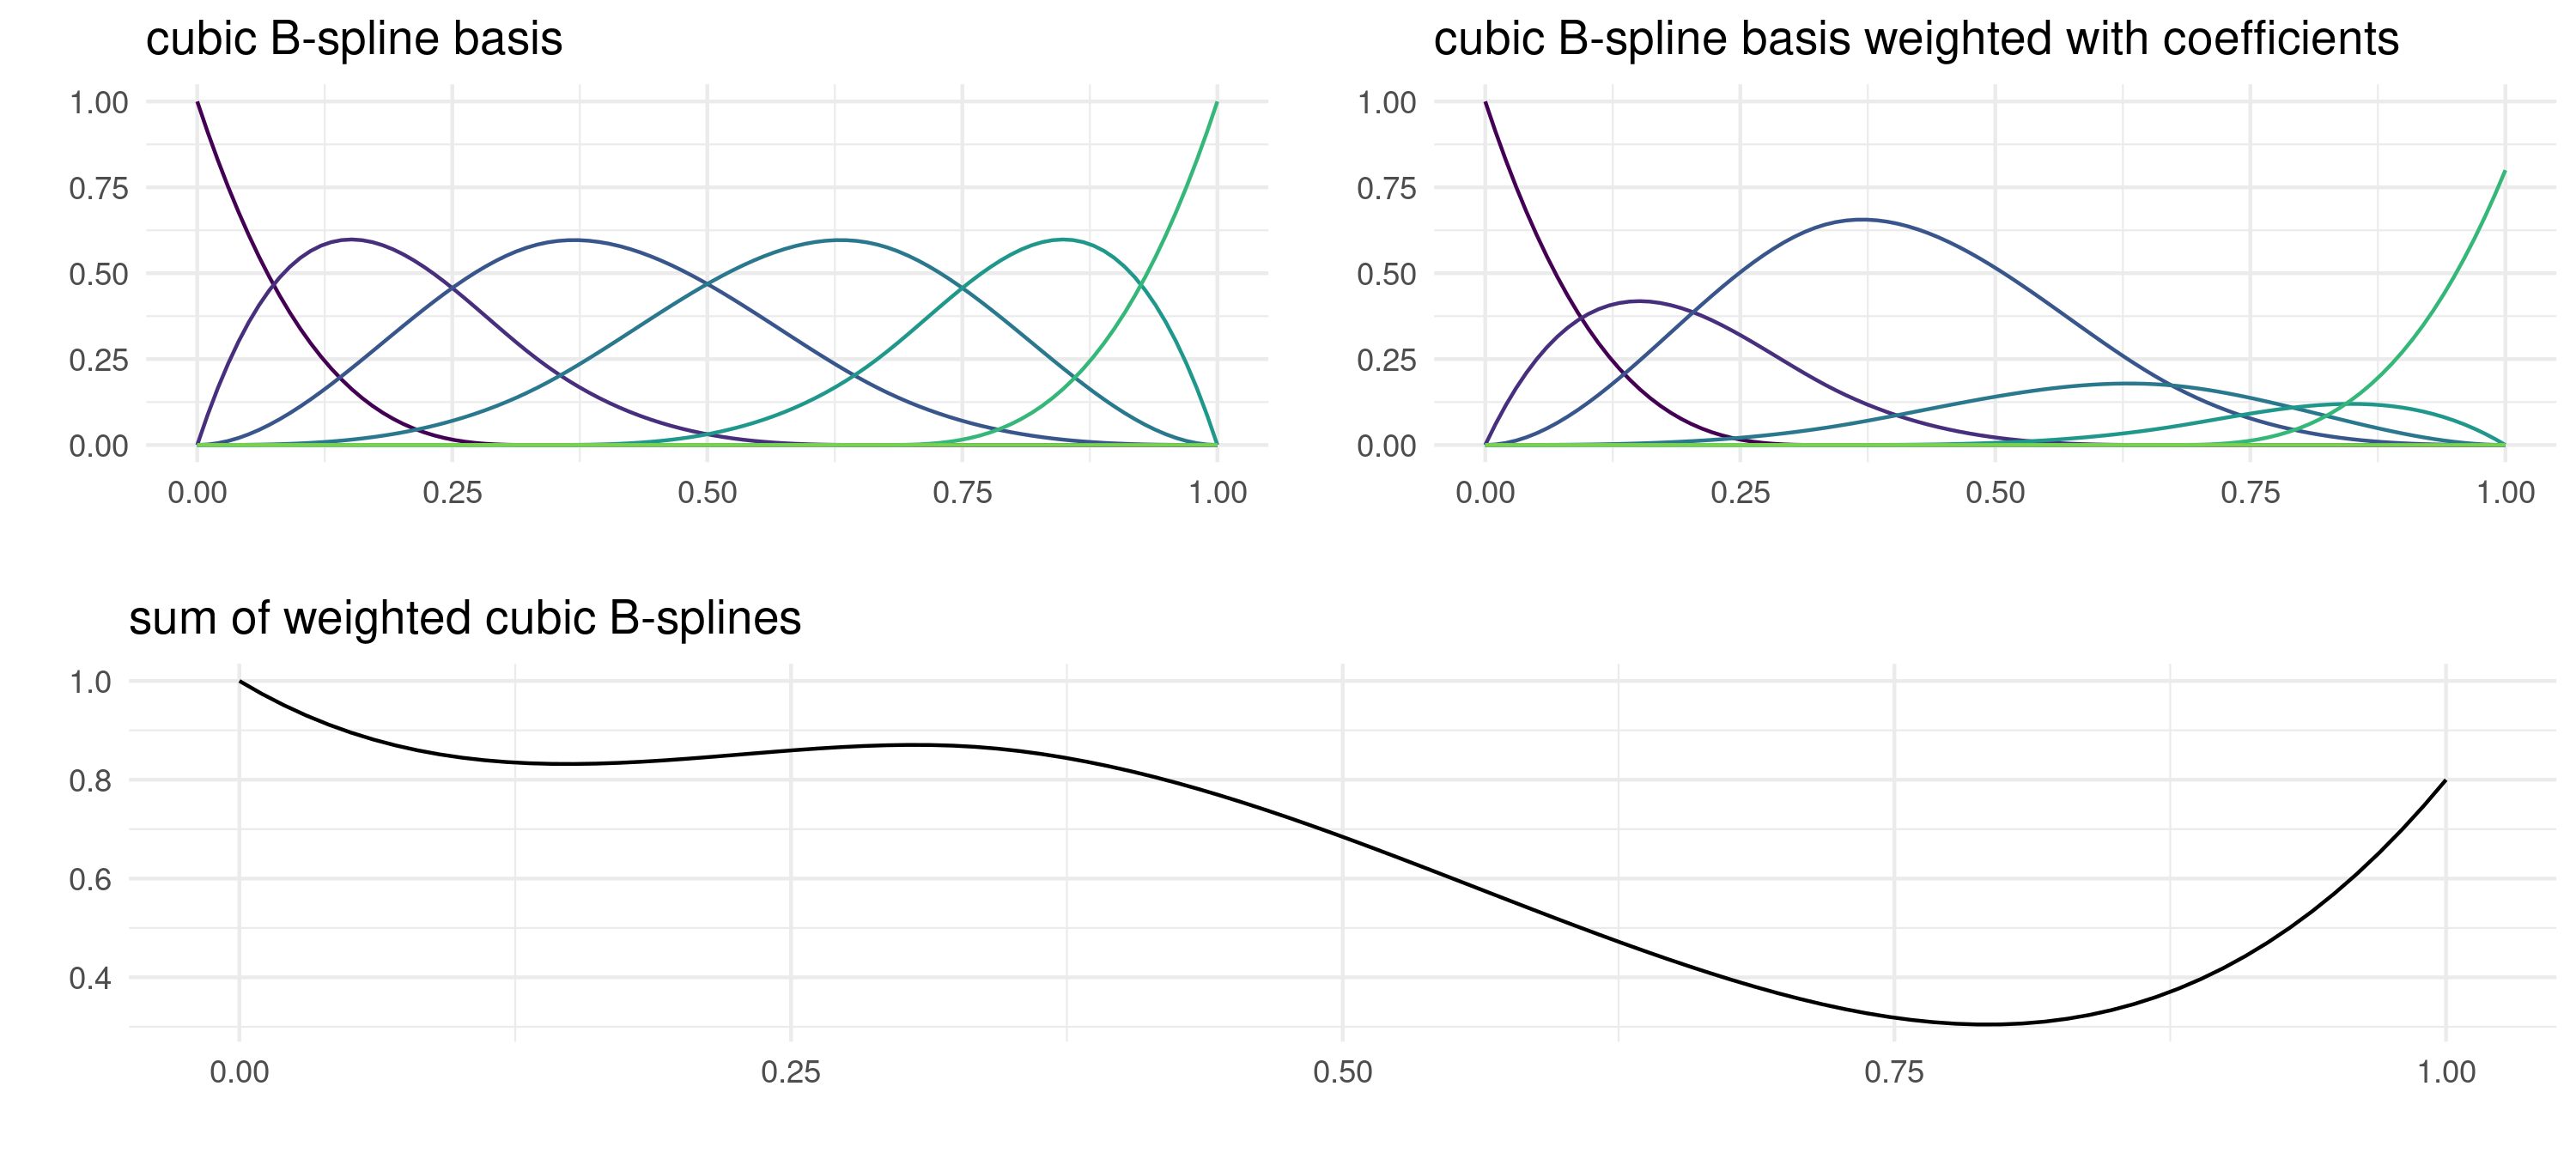
\includegraphics[width=0.9\textwidth]{figure/bspline-basis.png}
\end{center}

% \vfill
%
% \begin{center}
% \includegraphics[width=1\textwidth]{figure_man/NBL02.png}
% \end{center}

\end{vbframe}

% ------------------------------------------------------------------------------

% tex file and figures are created automatically by: rsrc/fig-cwb-anim-nl.R

\begin{frame}{Example: Life expectancy (nonlinear)}
	\begin{figure}
		\centering
		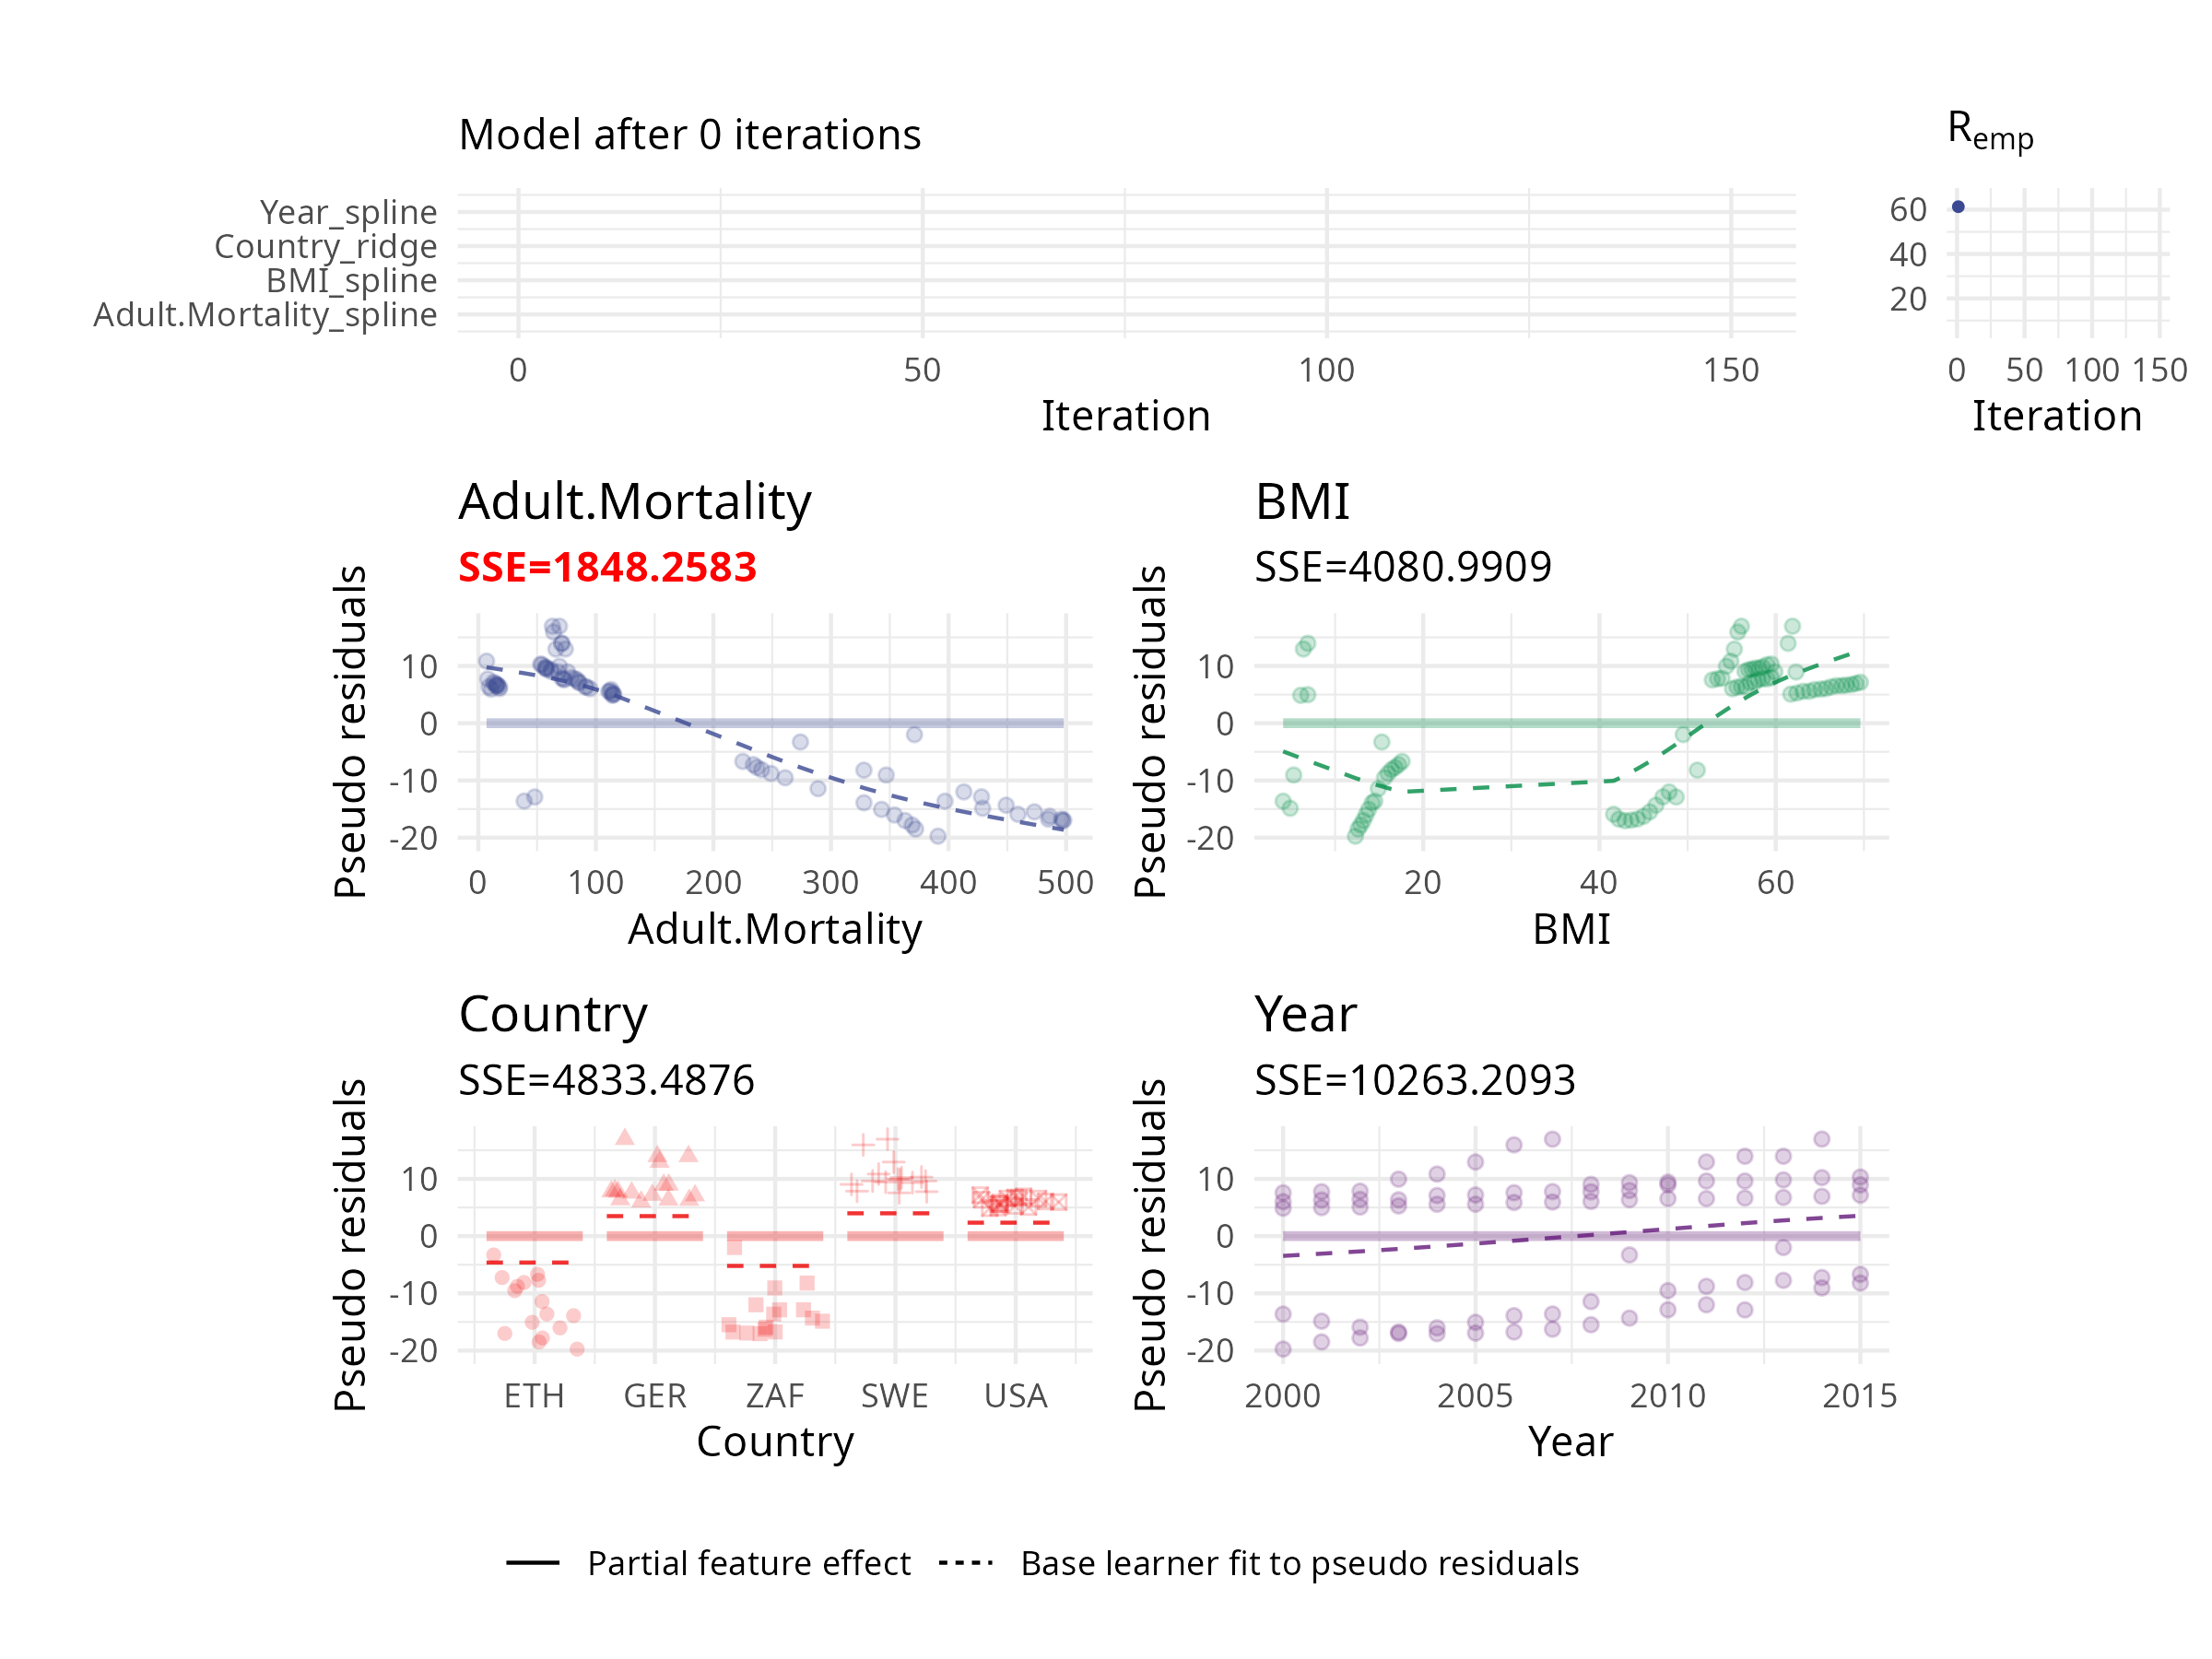
\includegraphics[width=\textwidth]{figure/cwb-anim-nl/fig-iter-0001.png}
	\end{figure}
	\addtocounter{framenumber}{0}
\end{frame}


\begin{frame}{Example: Life expectancy (nonlinear)}
	\begin{figure}
		\centering
		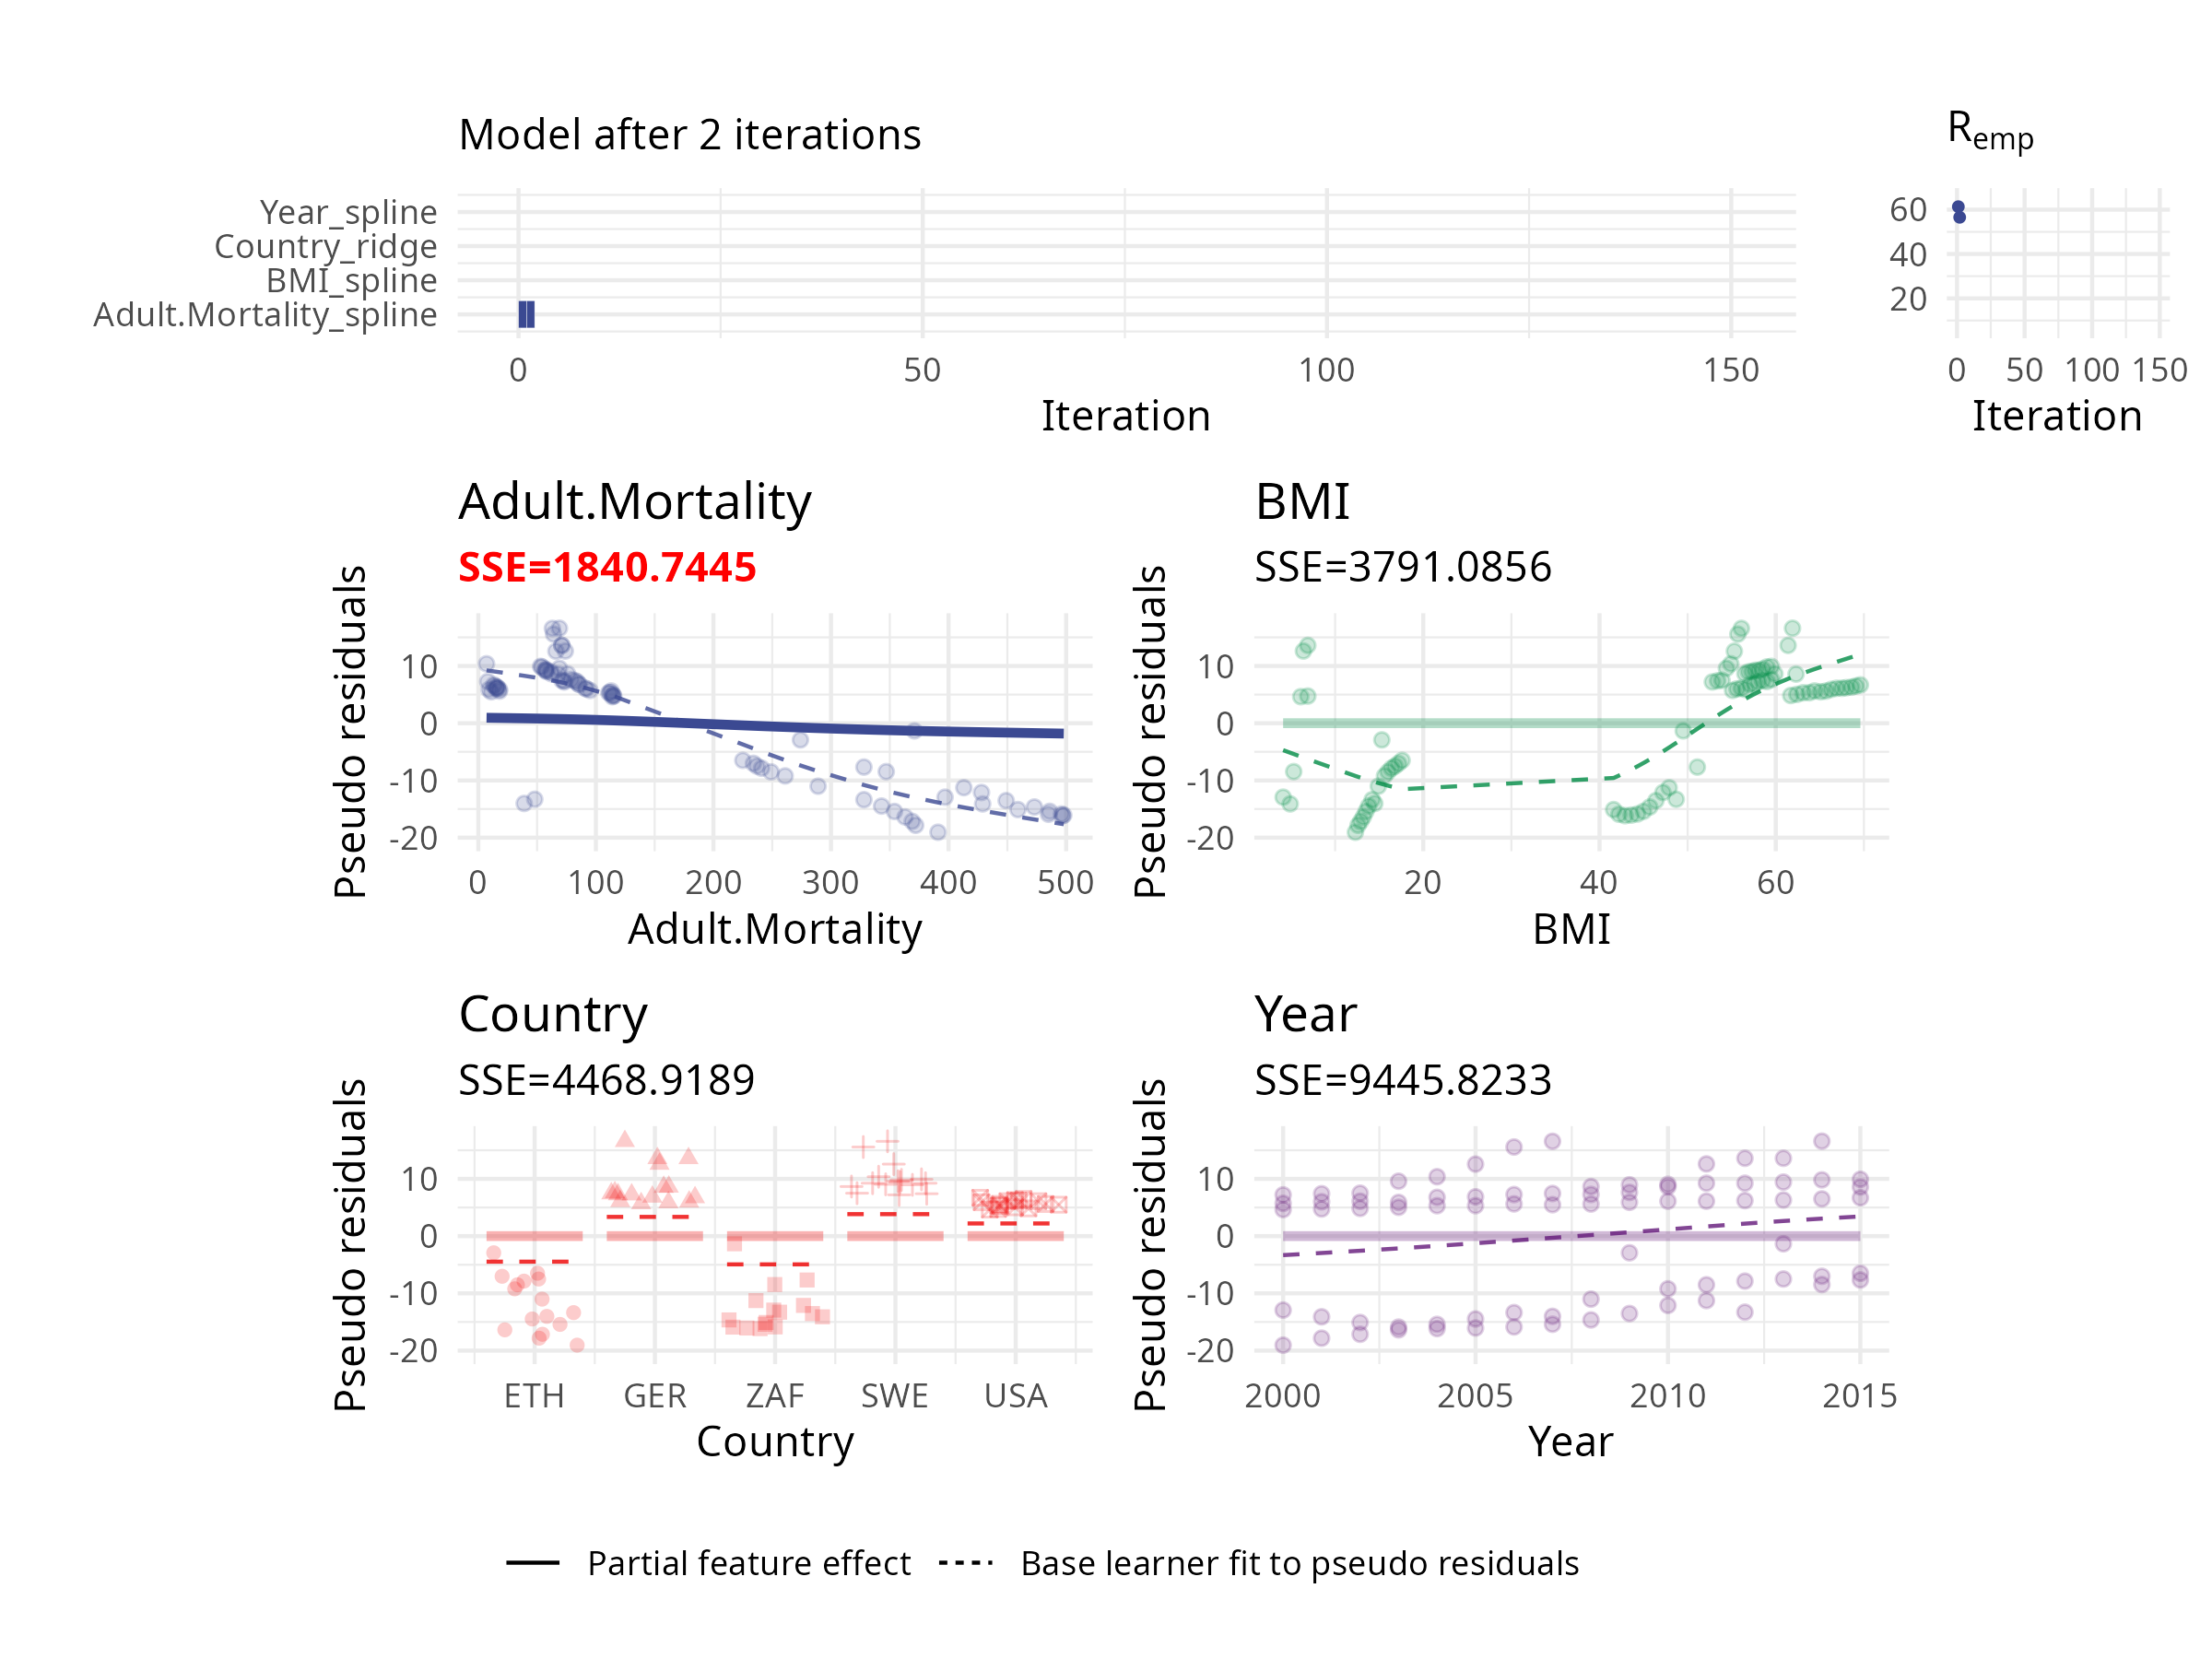
\includegraphics[width=\textwidth]{figure/cwb-anim-nl/fig-iter-0002.png}
	\end{figure}
	\addtocounter{framenumber}{-1}
\end{frame}


\begin{frame}{Example: Life expectancy (nonlinear)}
	\begin{figure}
		\centering
		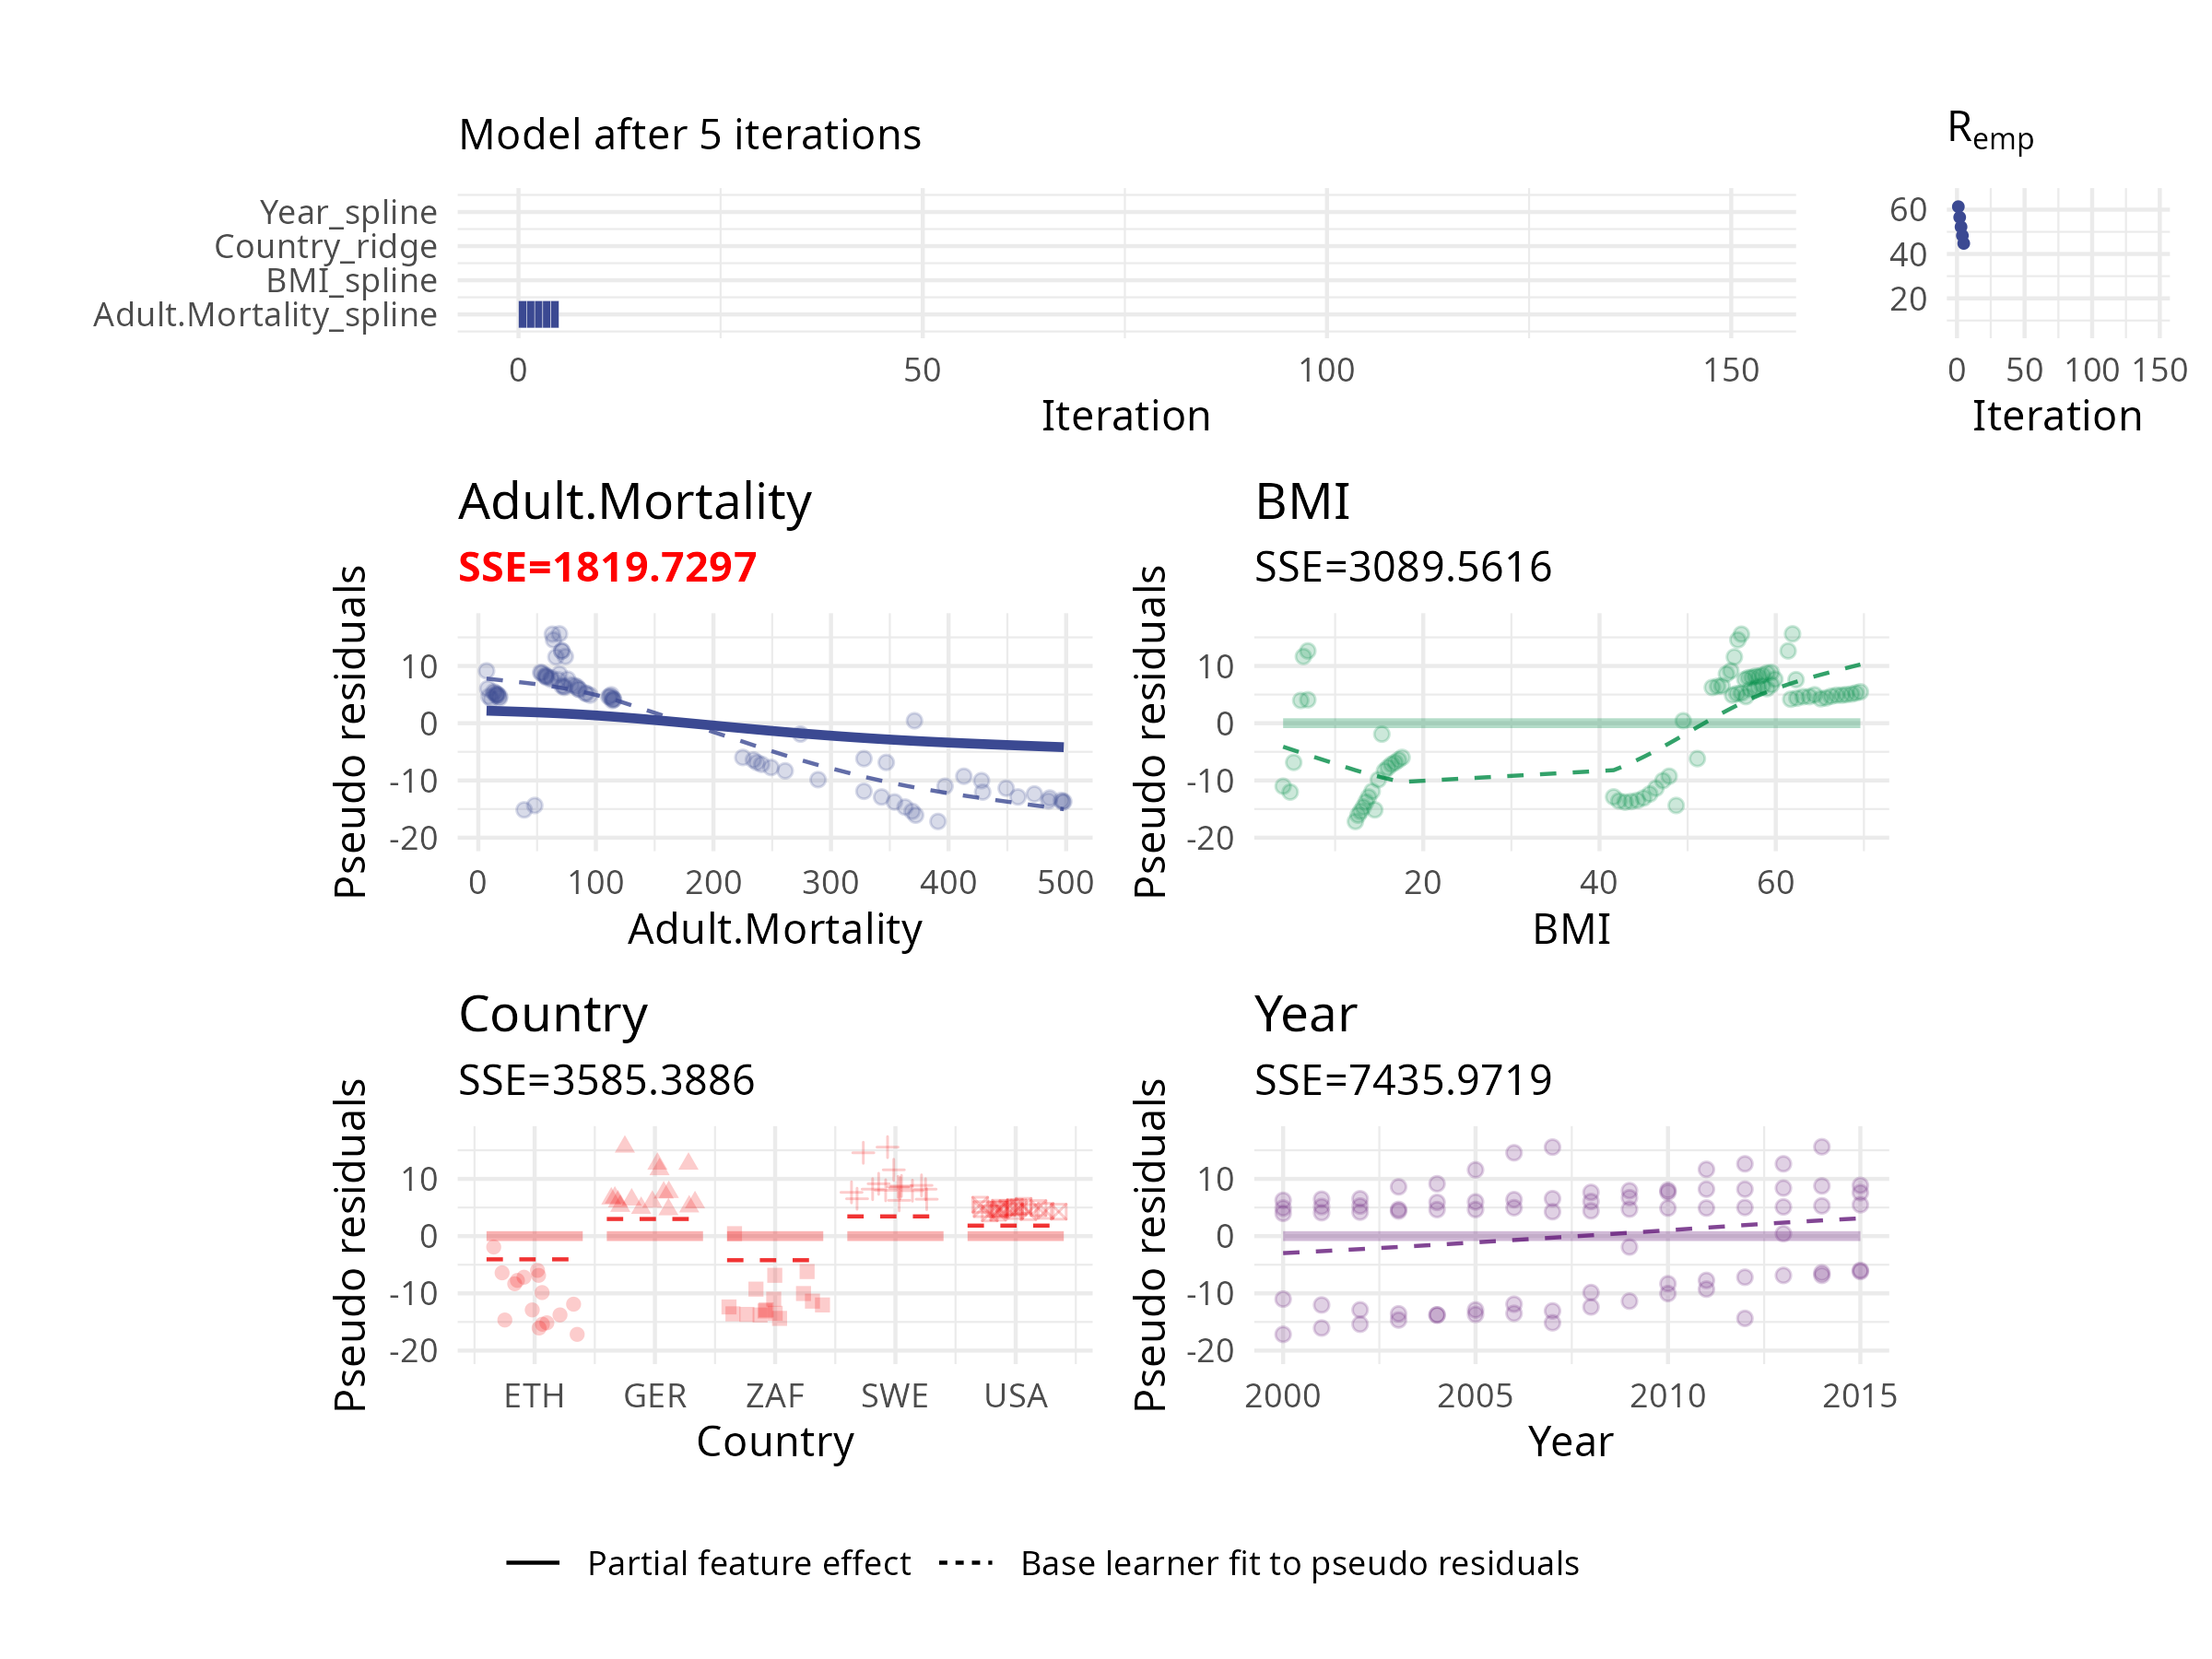
\includegraphics[width=\textwidth]{figure/cwb-anim-nl/fig-iter-0005.png}
	\end{figure}
	\addtocounter{framenumber}{-1}
\end{frame}


\begin{frame}{Example: Life expectancy (nonlinear)}
	\begin{figure}
		\centering
		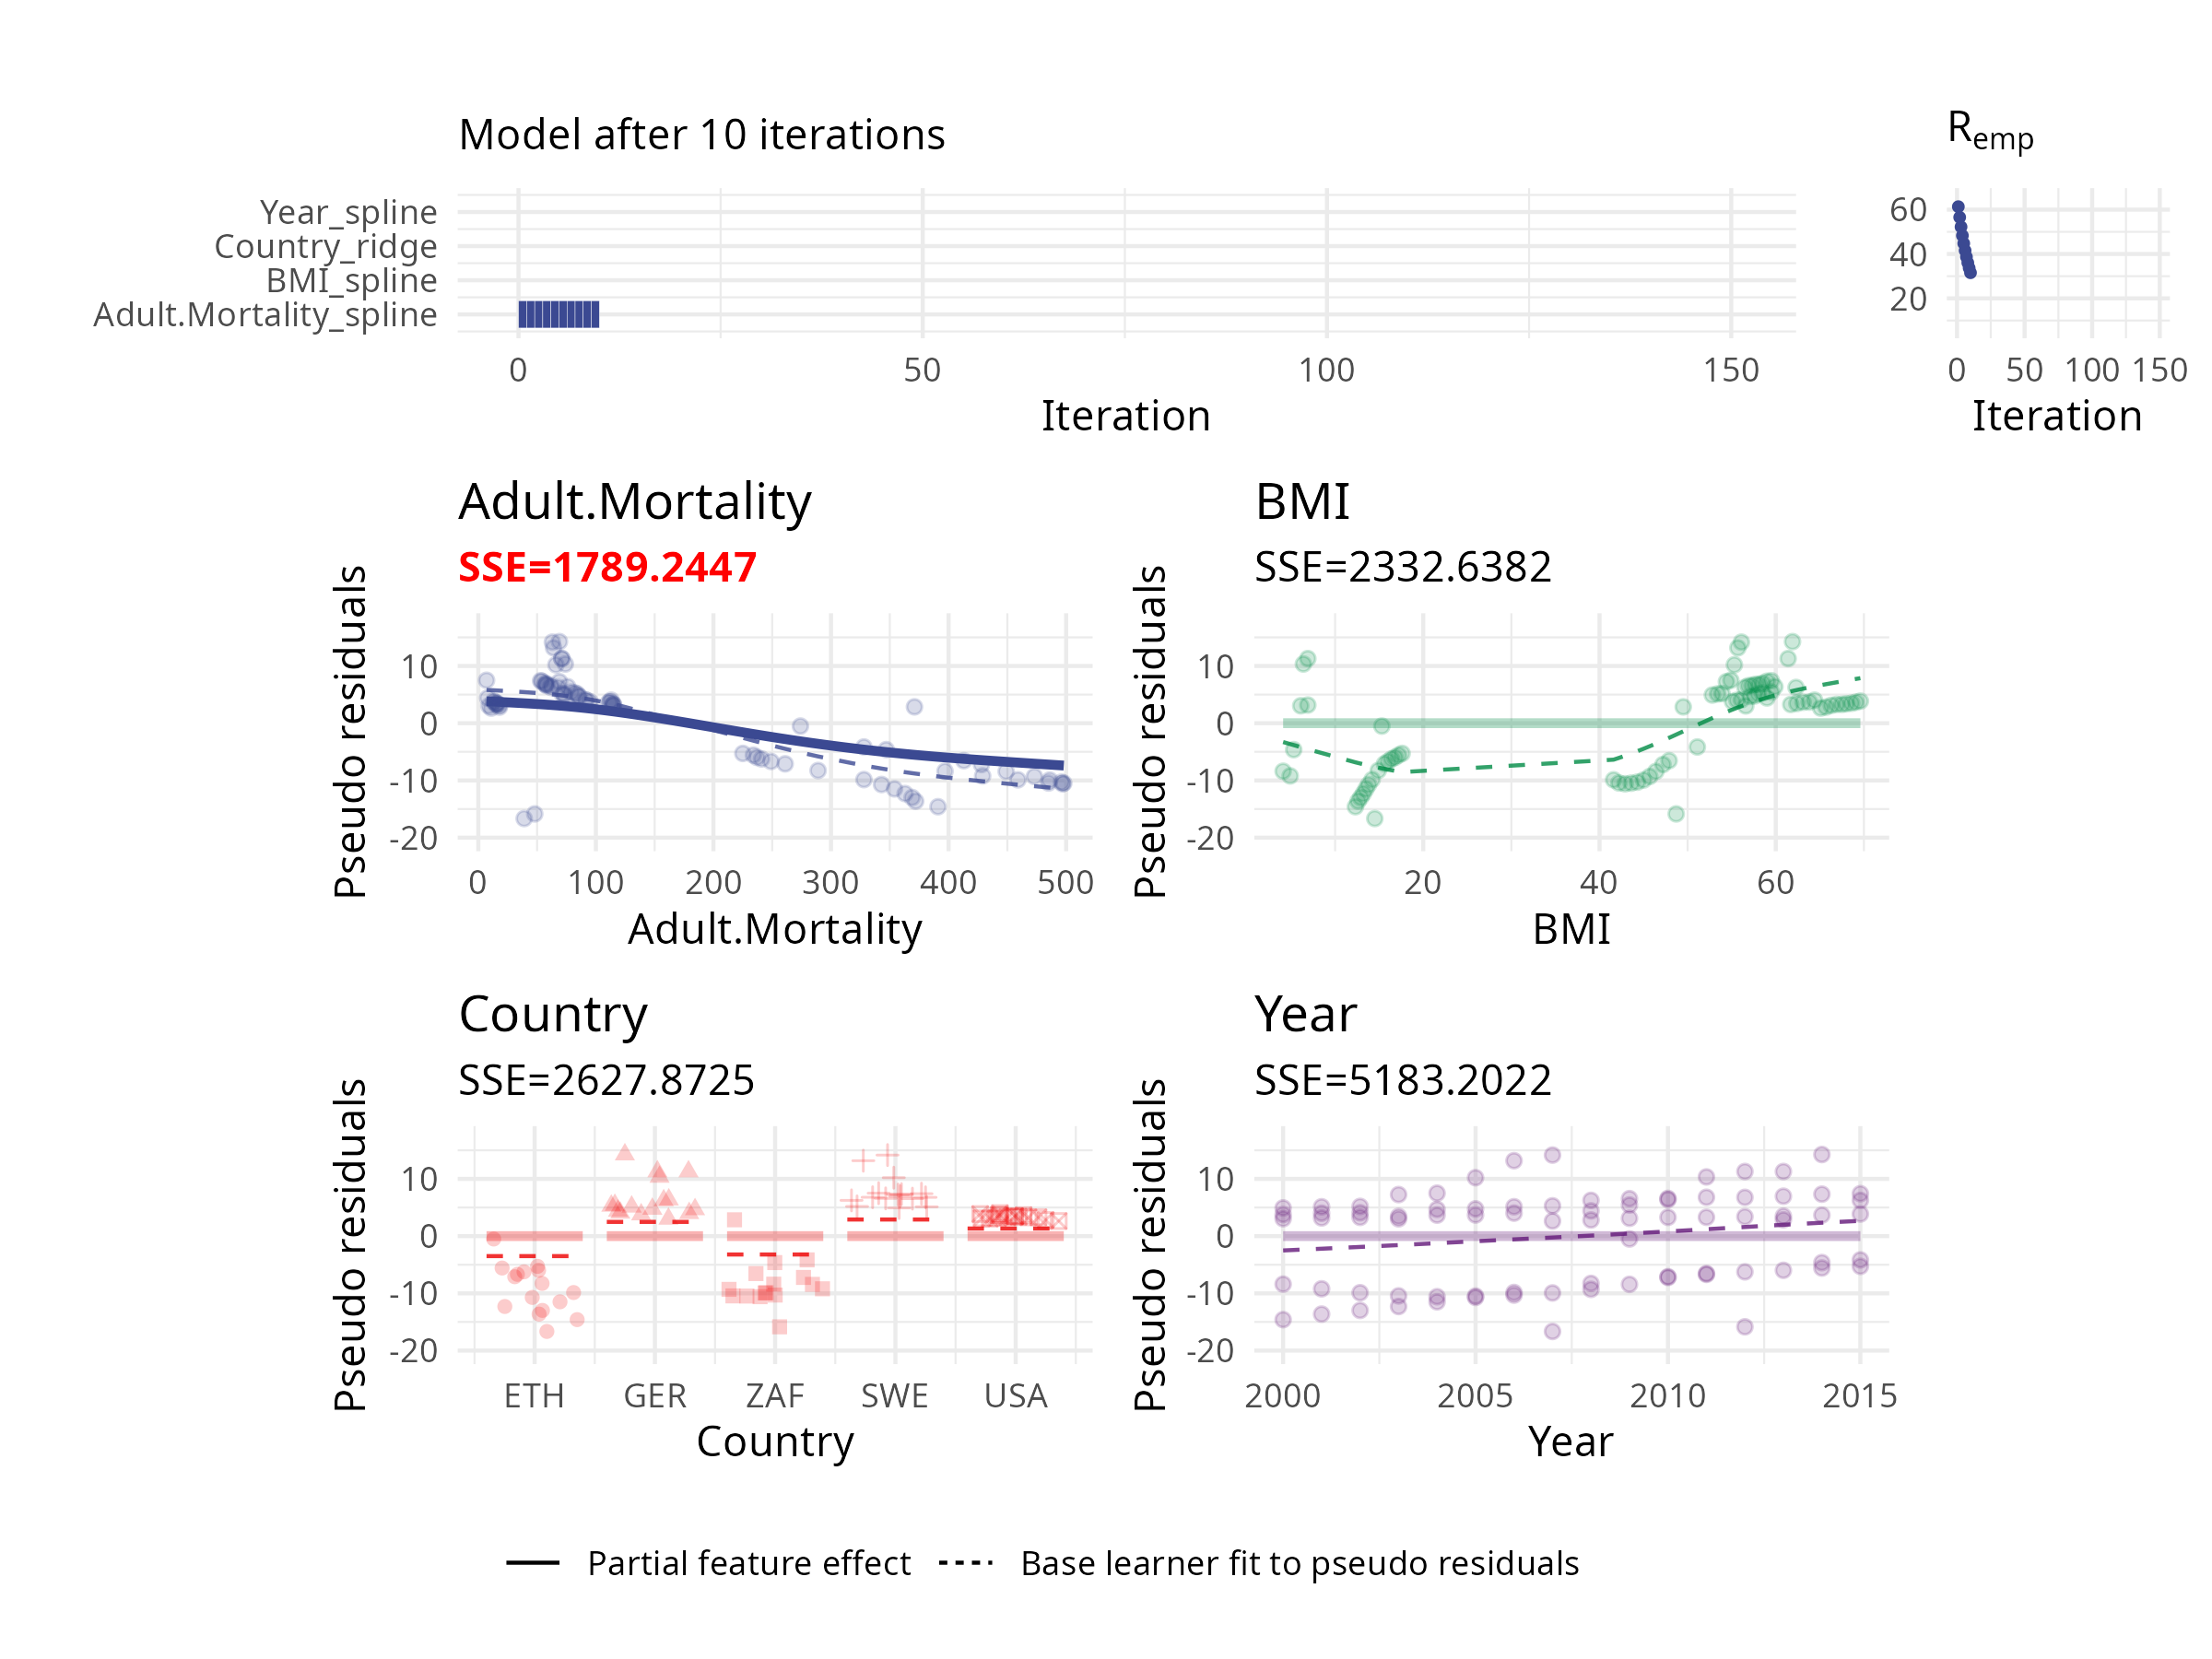
\includegraphics[width=\textwidth]{figure/cwb-anim-nl/fig-iter-0010.png}
	\end{figure}
	\addtocounter{framenumber}{-1}
\end{frame}


\begin{frame}{Example: Life expectancy (nonlinear)}
	\begin{figure}
		\centering
		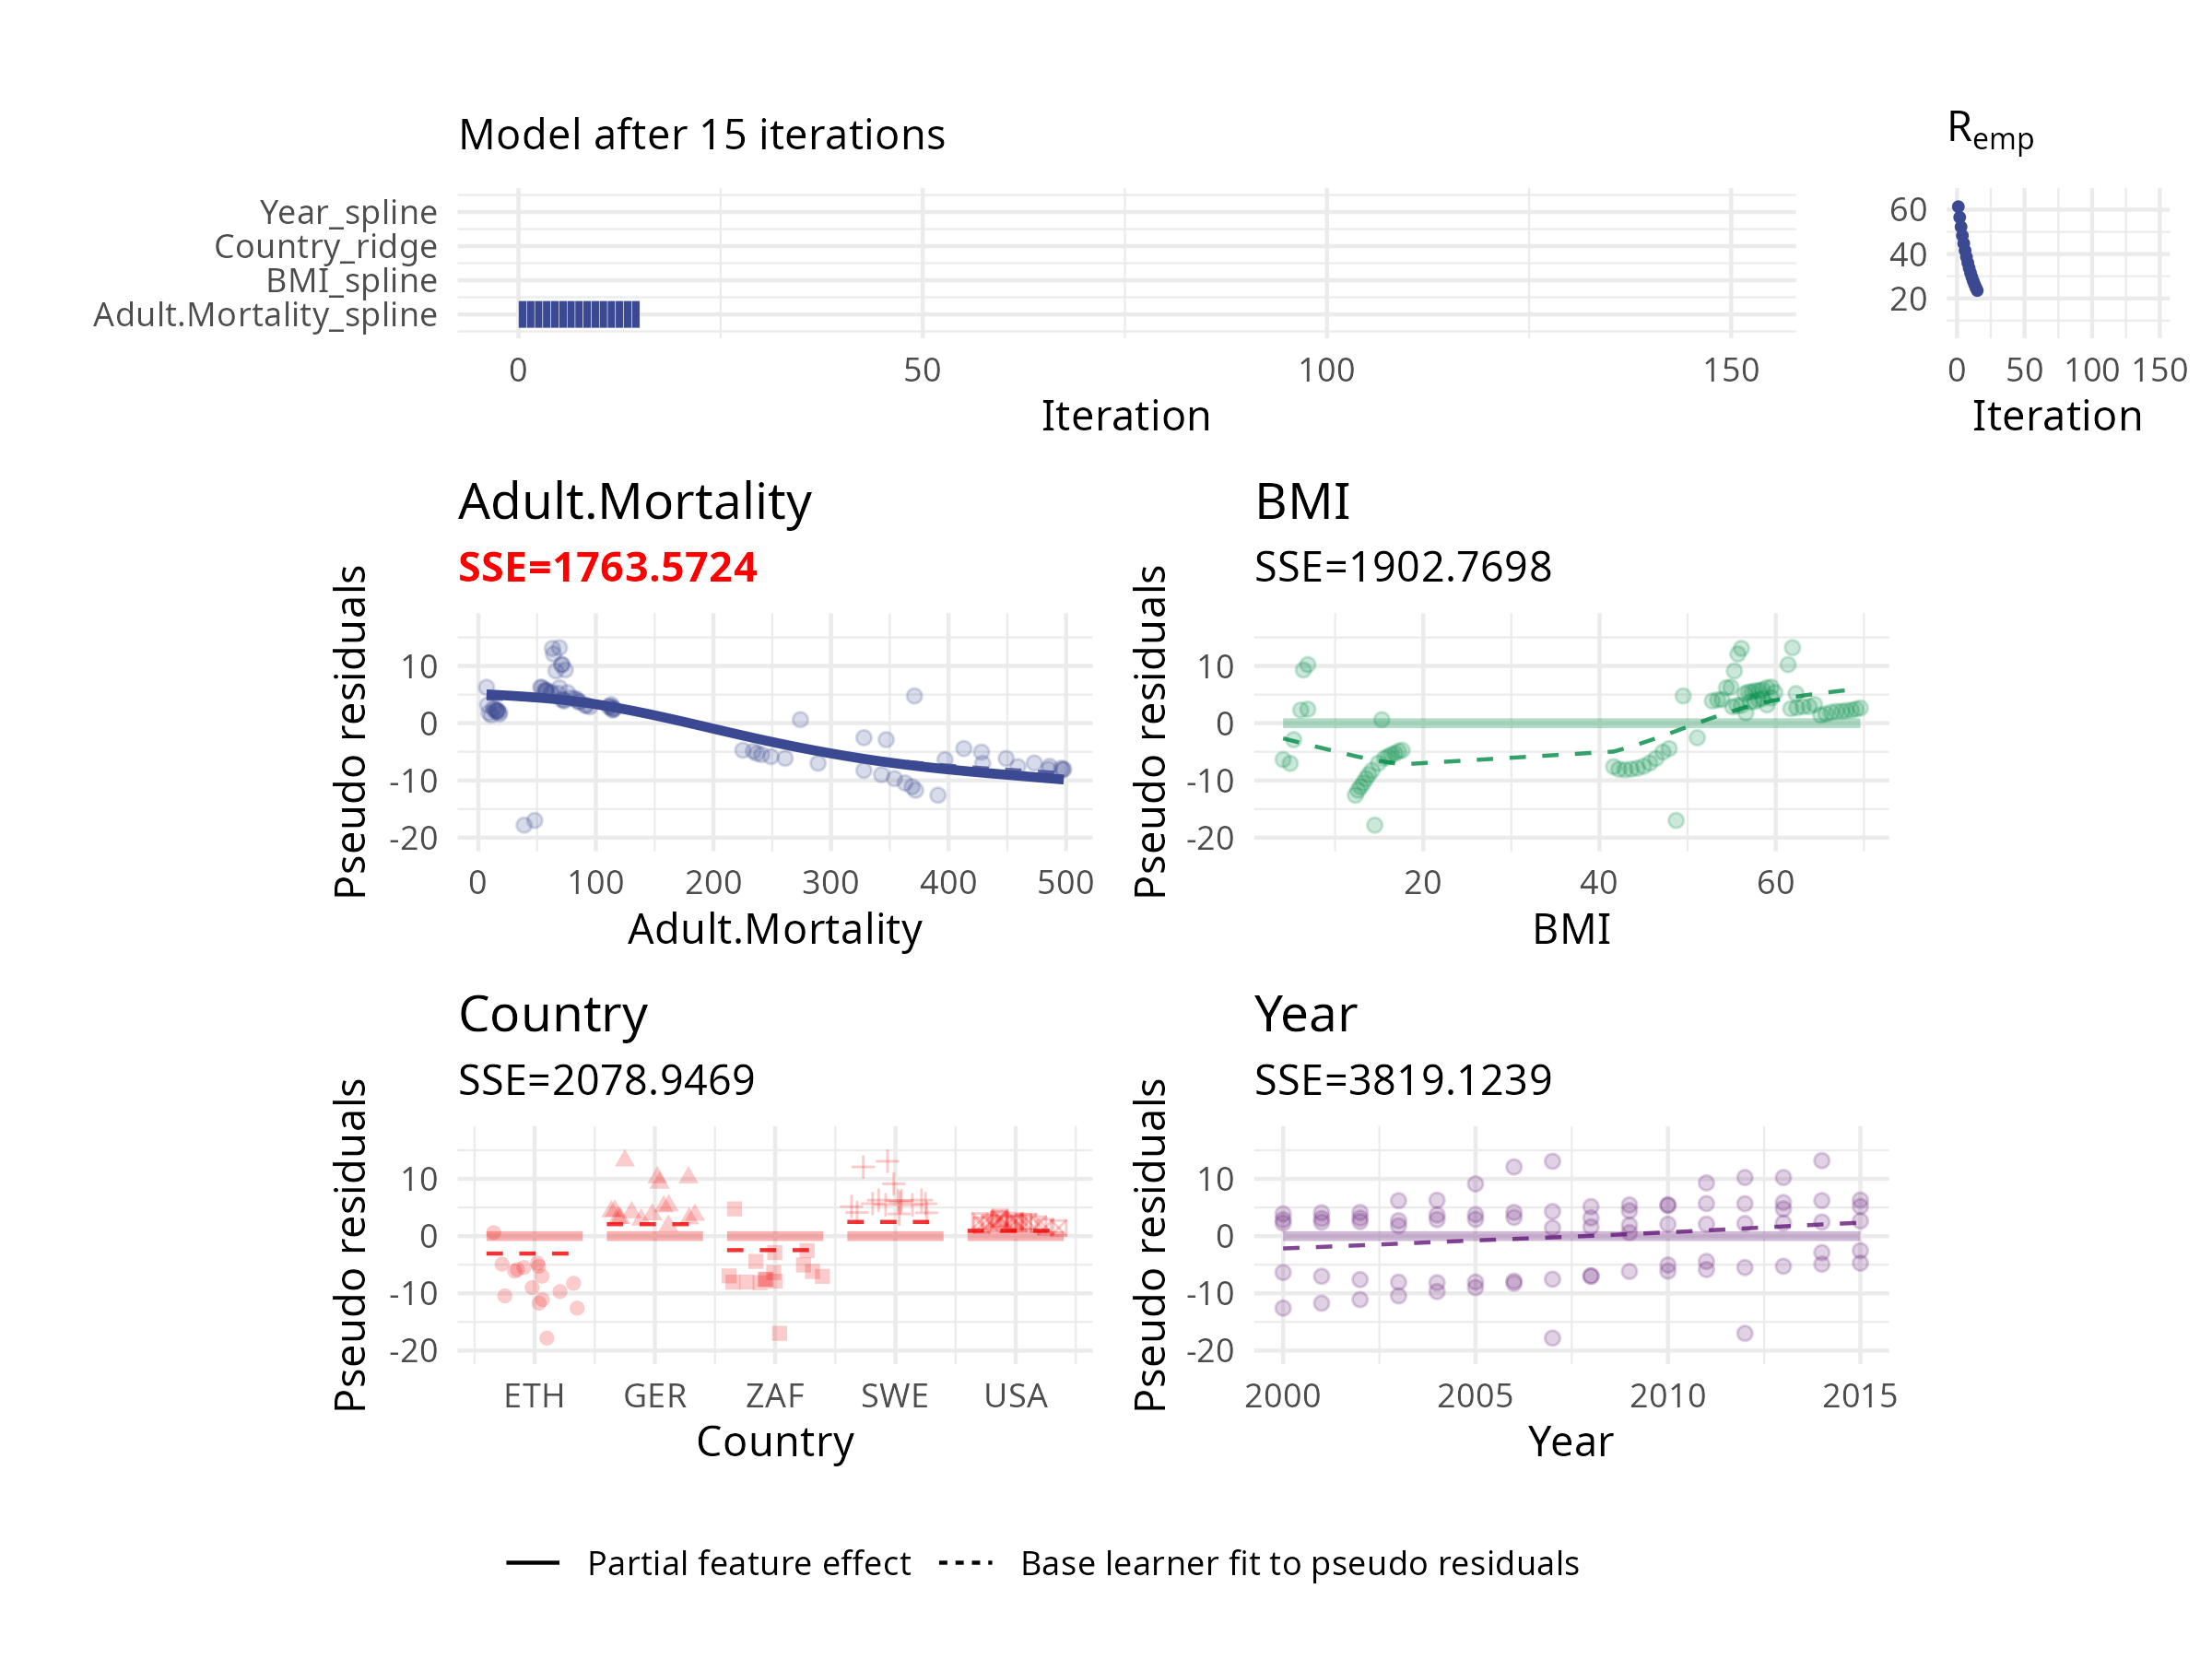
\includegraphics[width=\textwidth]{figure/cwb-anim-nl/fig-iter-0015.png}
	\end{figure}
	\addtocounter{framenumber}{-1}
\end{frame}


\begin{frame}{Example: Life expectancy (nonlinear)}
	\begin{figure}
		\centering
		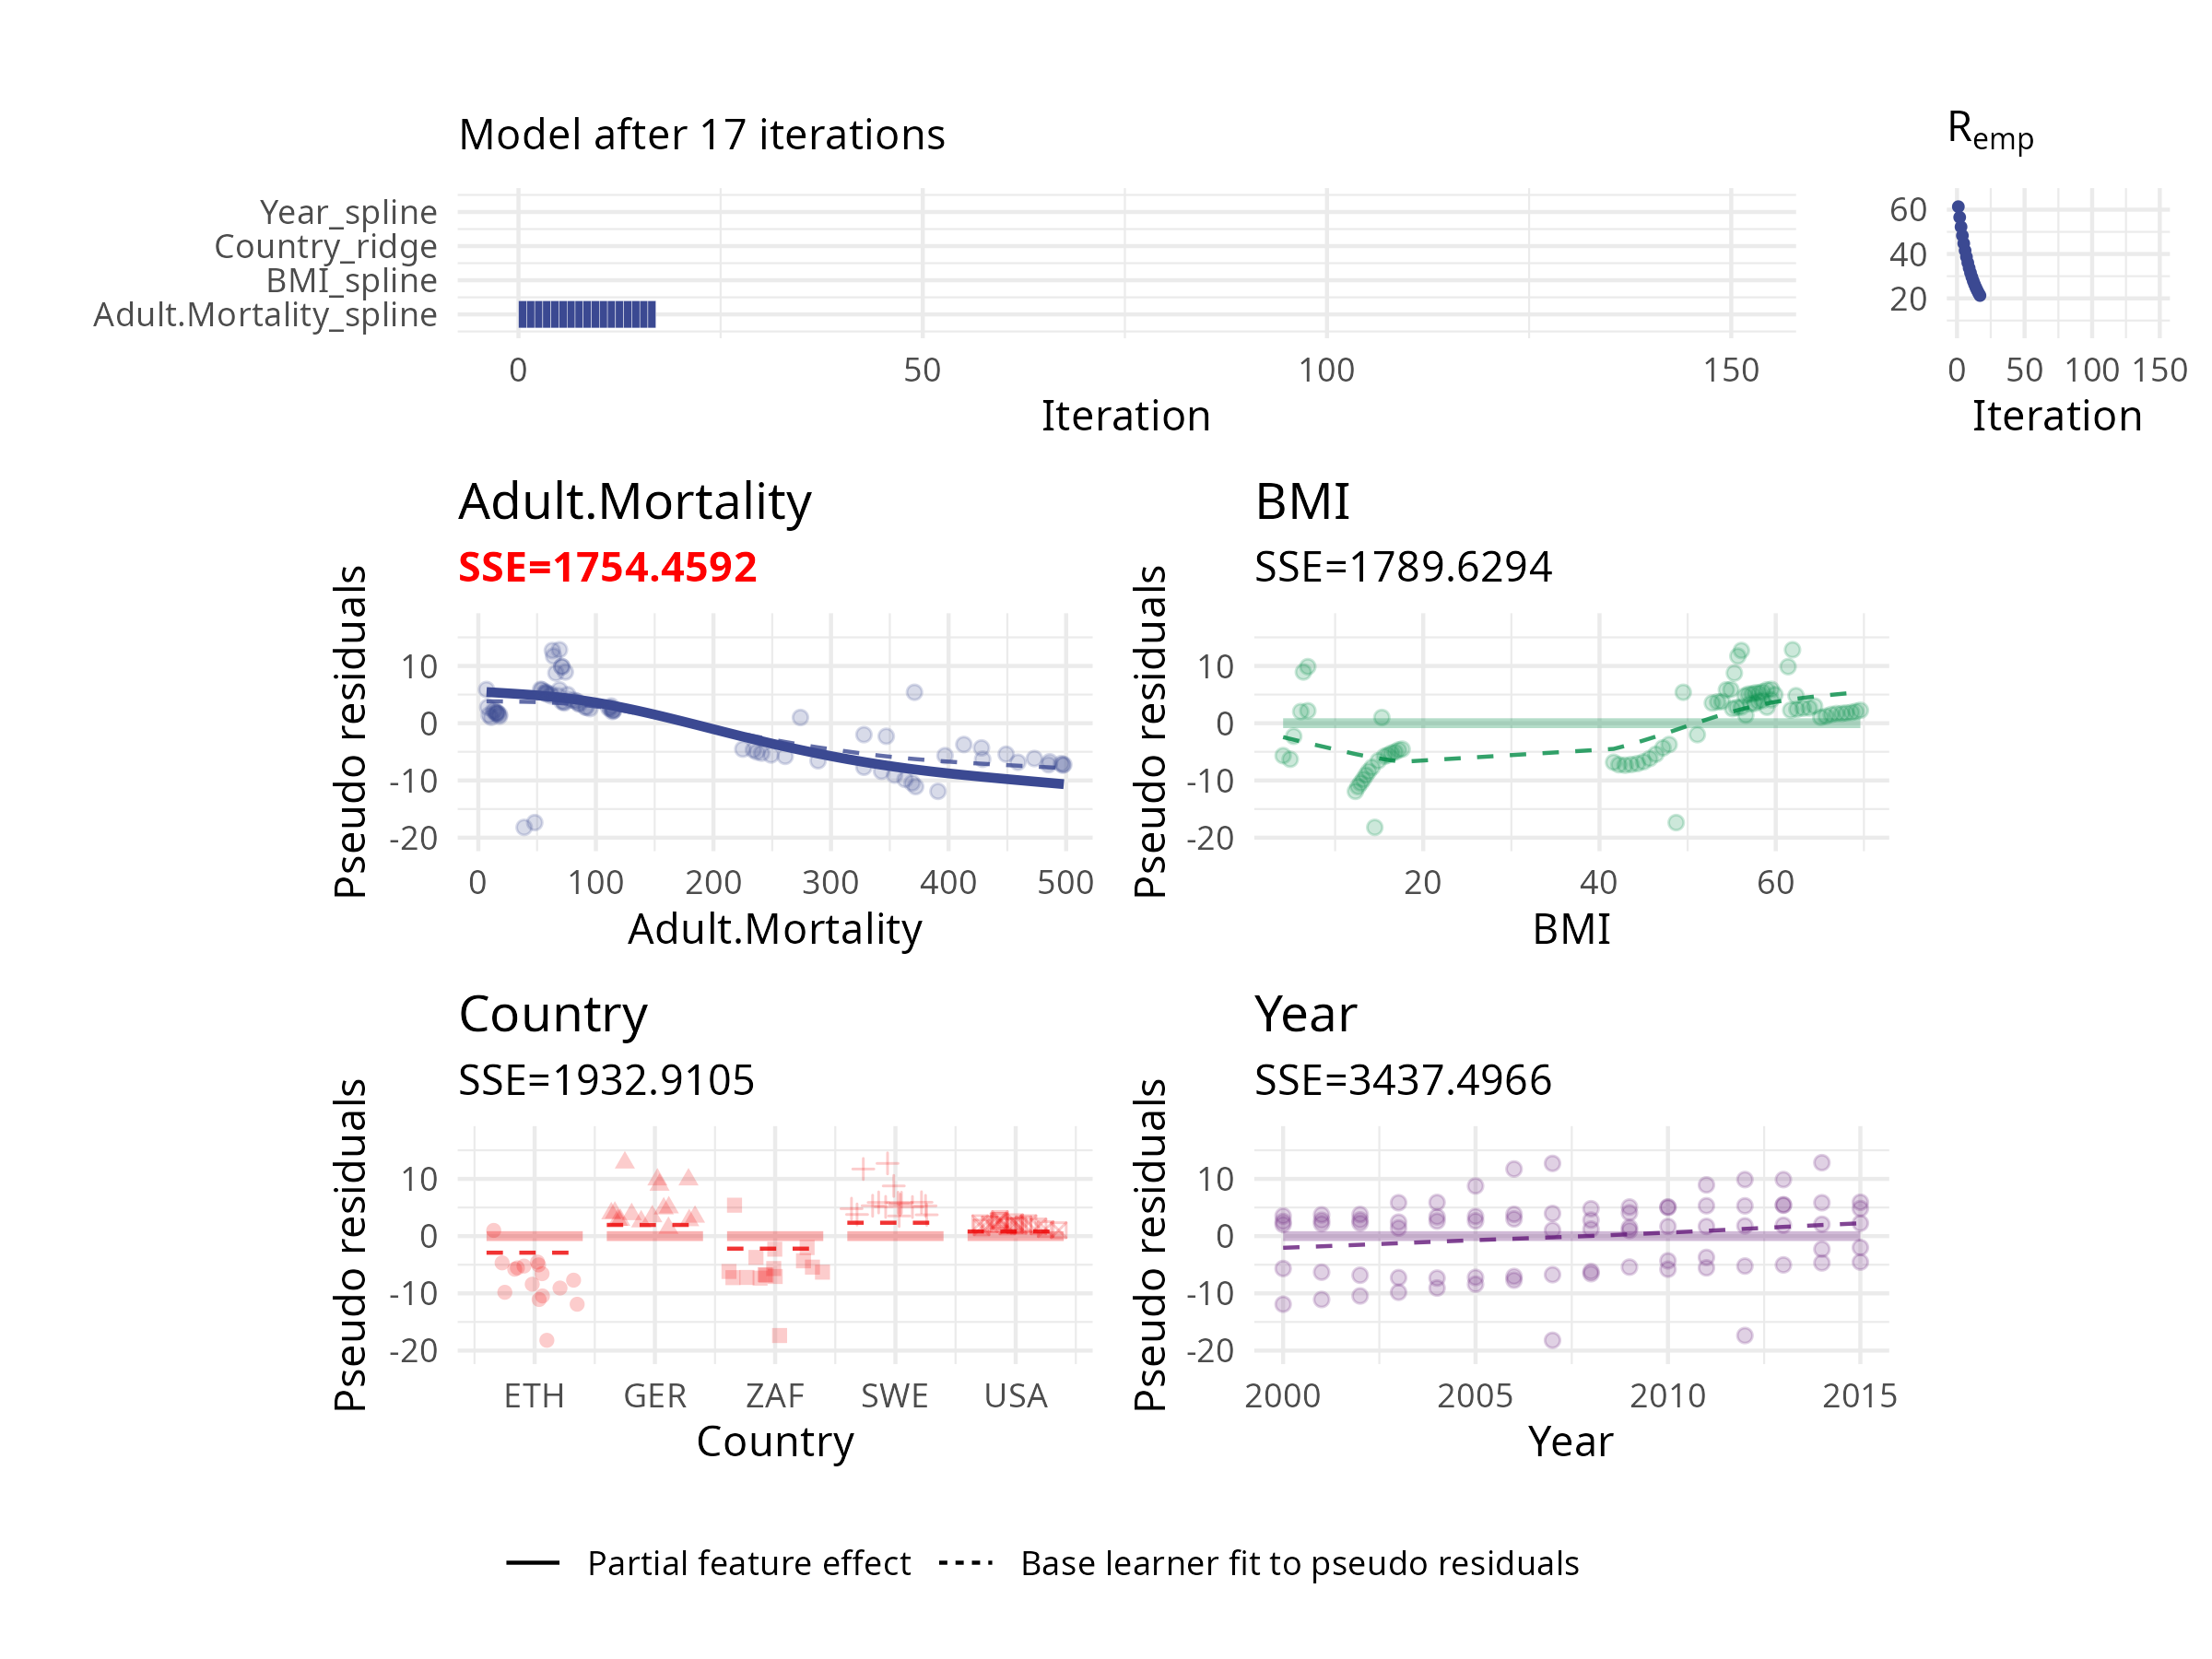
\includegraphics[width=\textwidth]{figure/cwb-anim-nl/fig-iter-0017.png}
	\end{figure}
	\addtocounter{framenumber}{-1}
\end{frame}


\begin{frame}{Example: Life expectancy (nonlinear)}
	\begin{figure}
		\centering
		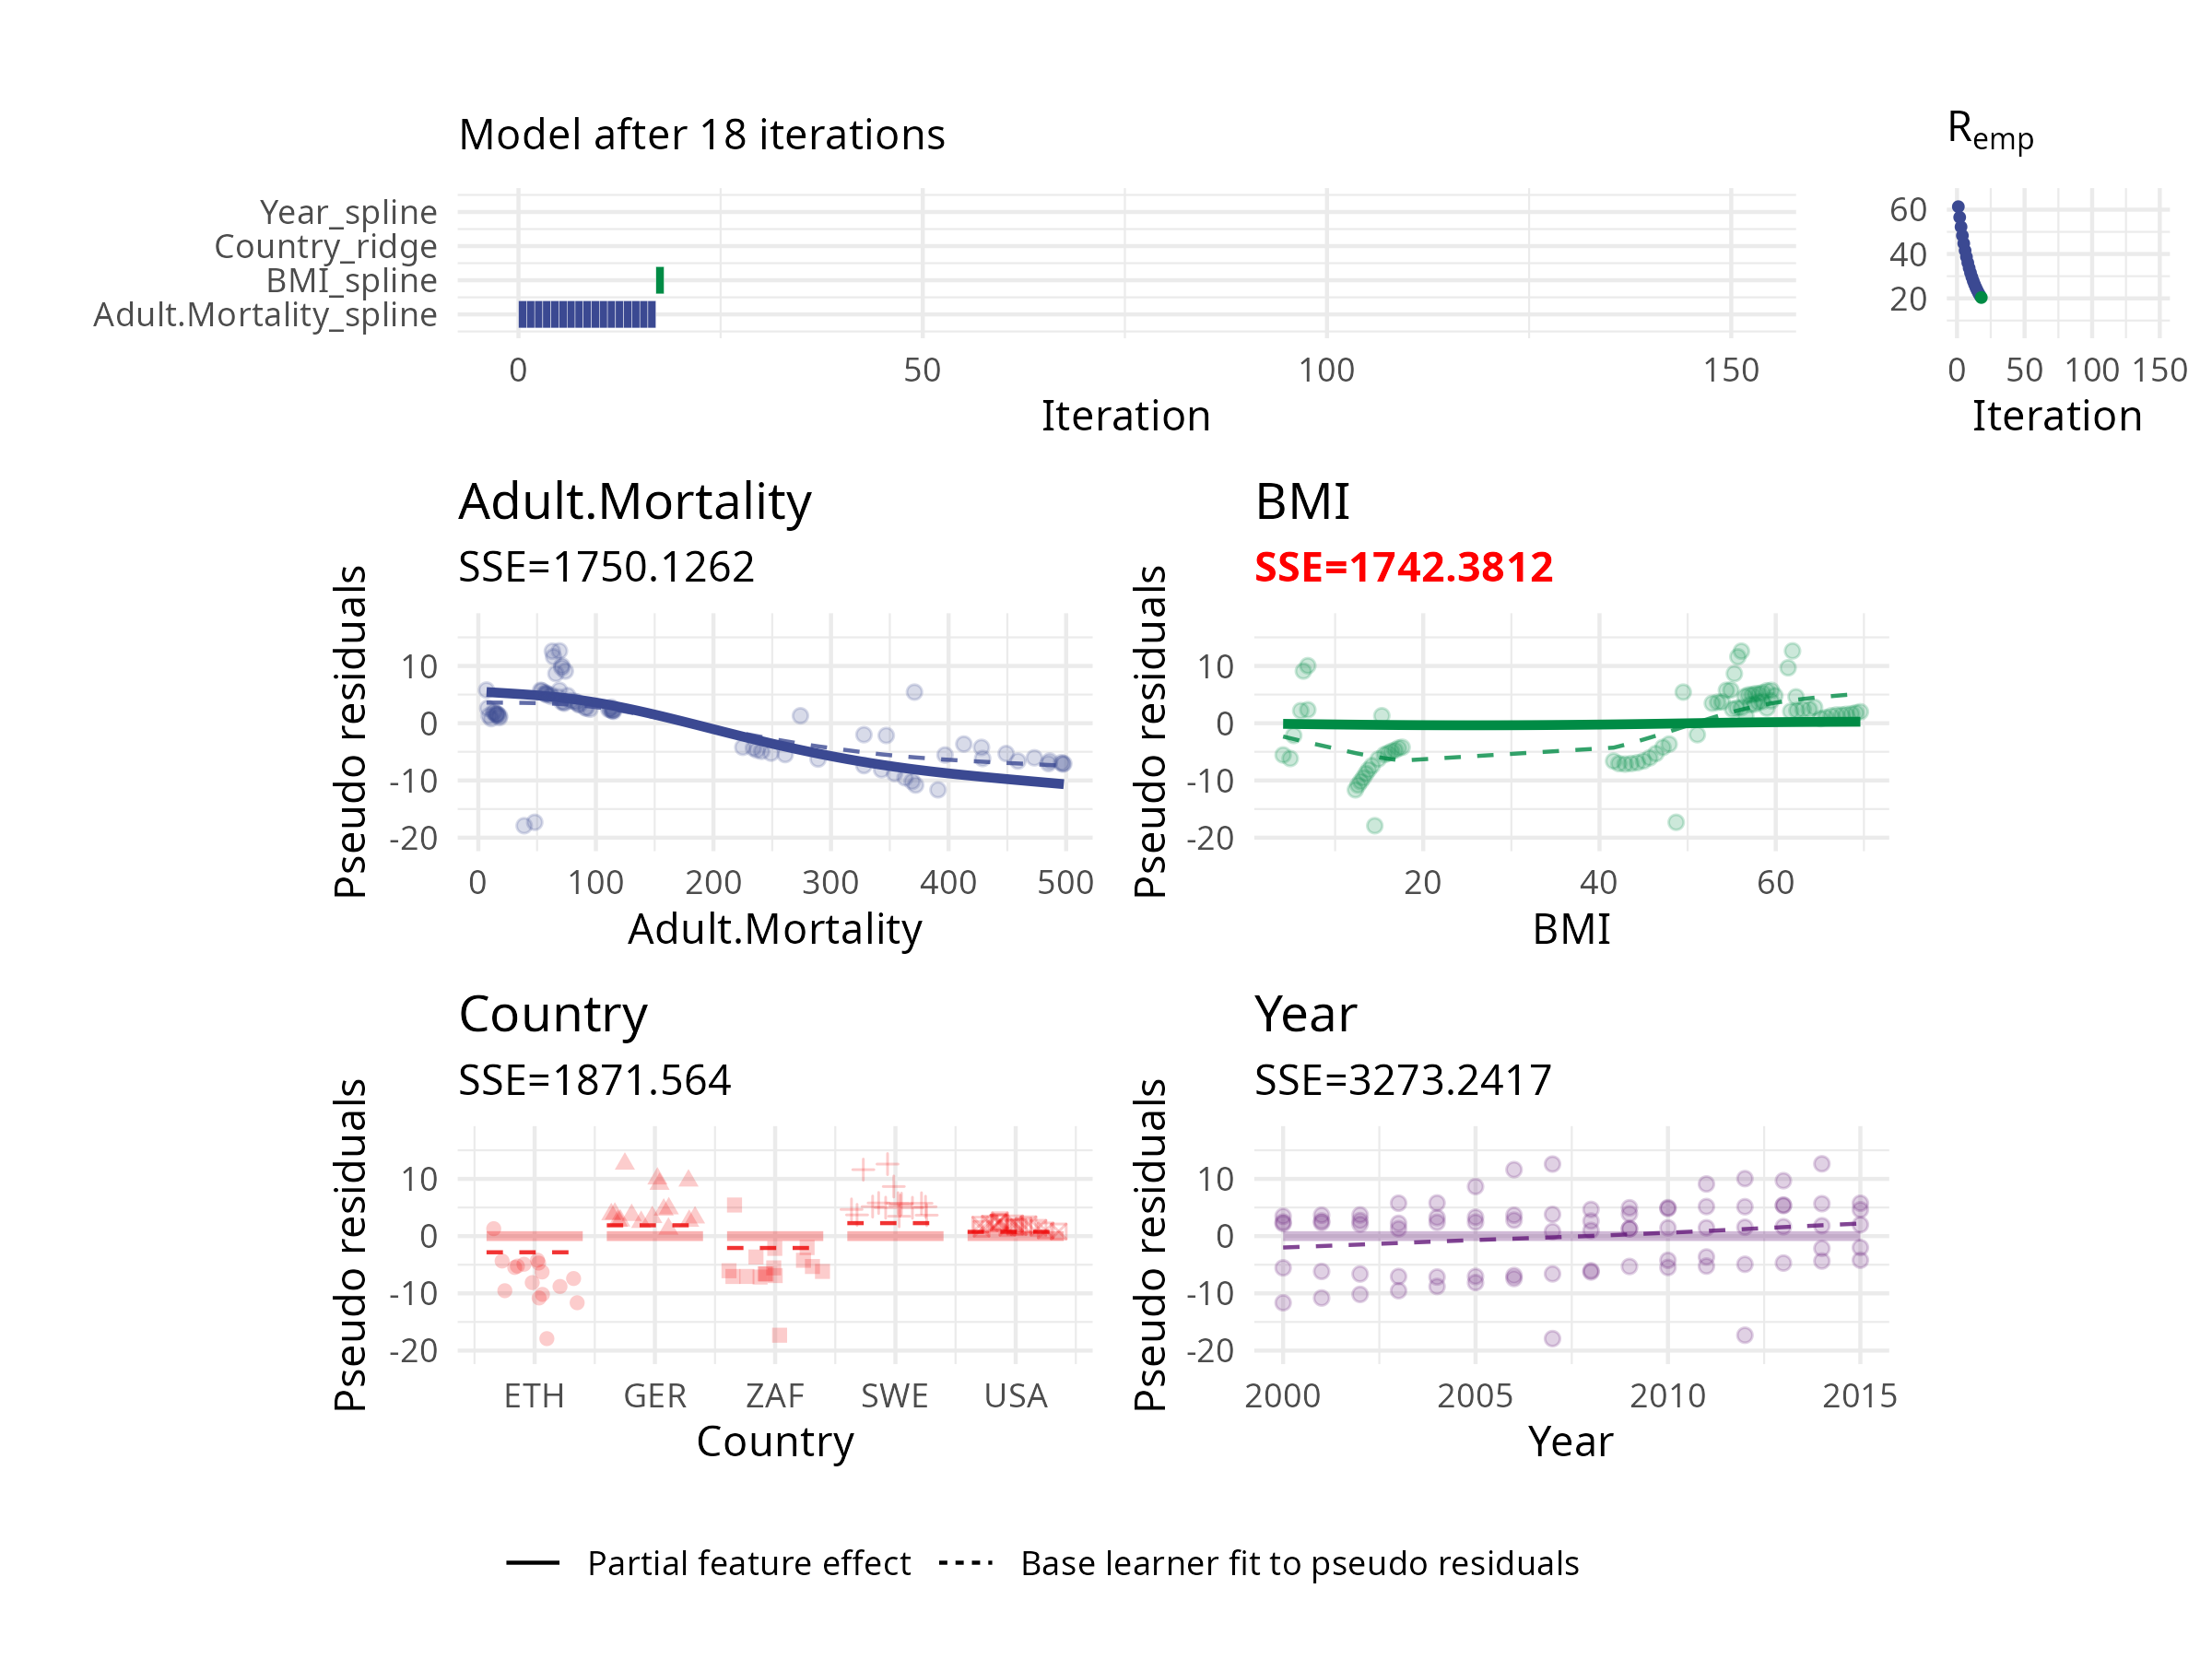
\includegraphics[width=\textwidth]{figure/cwb-anim-nl/fig-iter-0018.png}
	\end{figure}
	\addtocounter{framenumber}{-1}
\end{frame}


\begin{frame}{Example: Life expectancy (nonlinear)}
	\begin{figure}
		\centering
		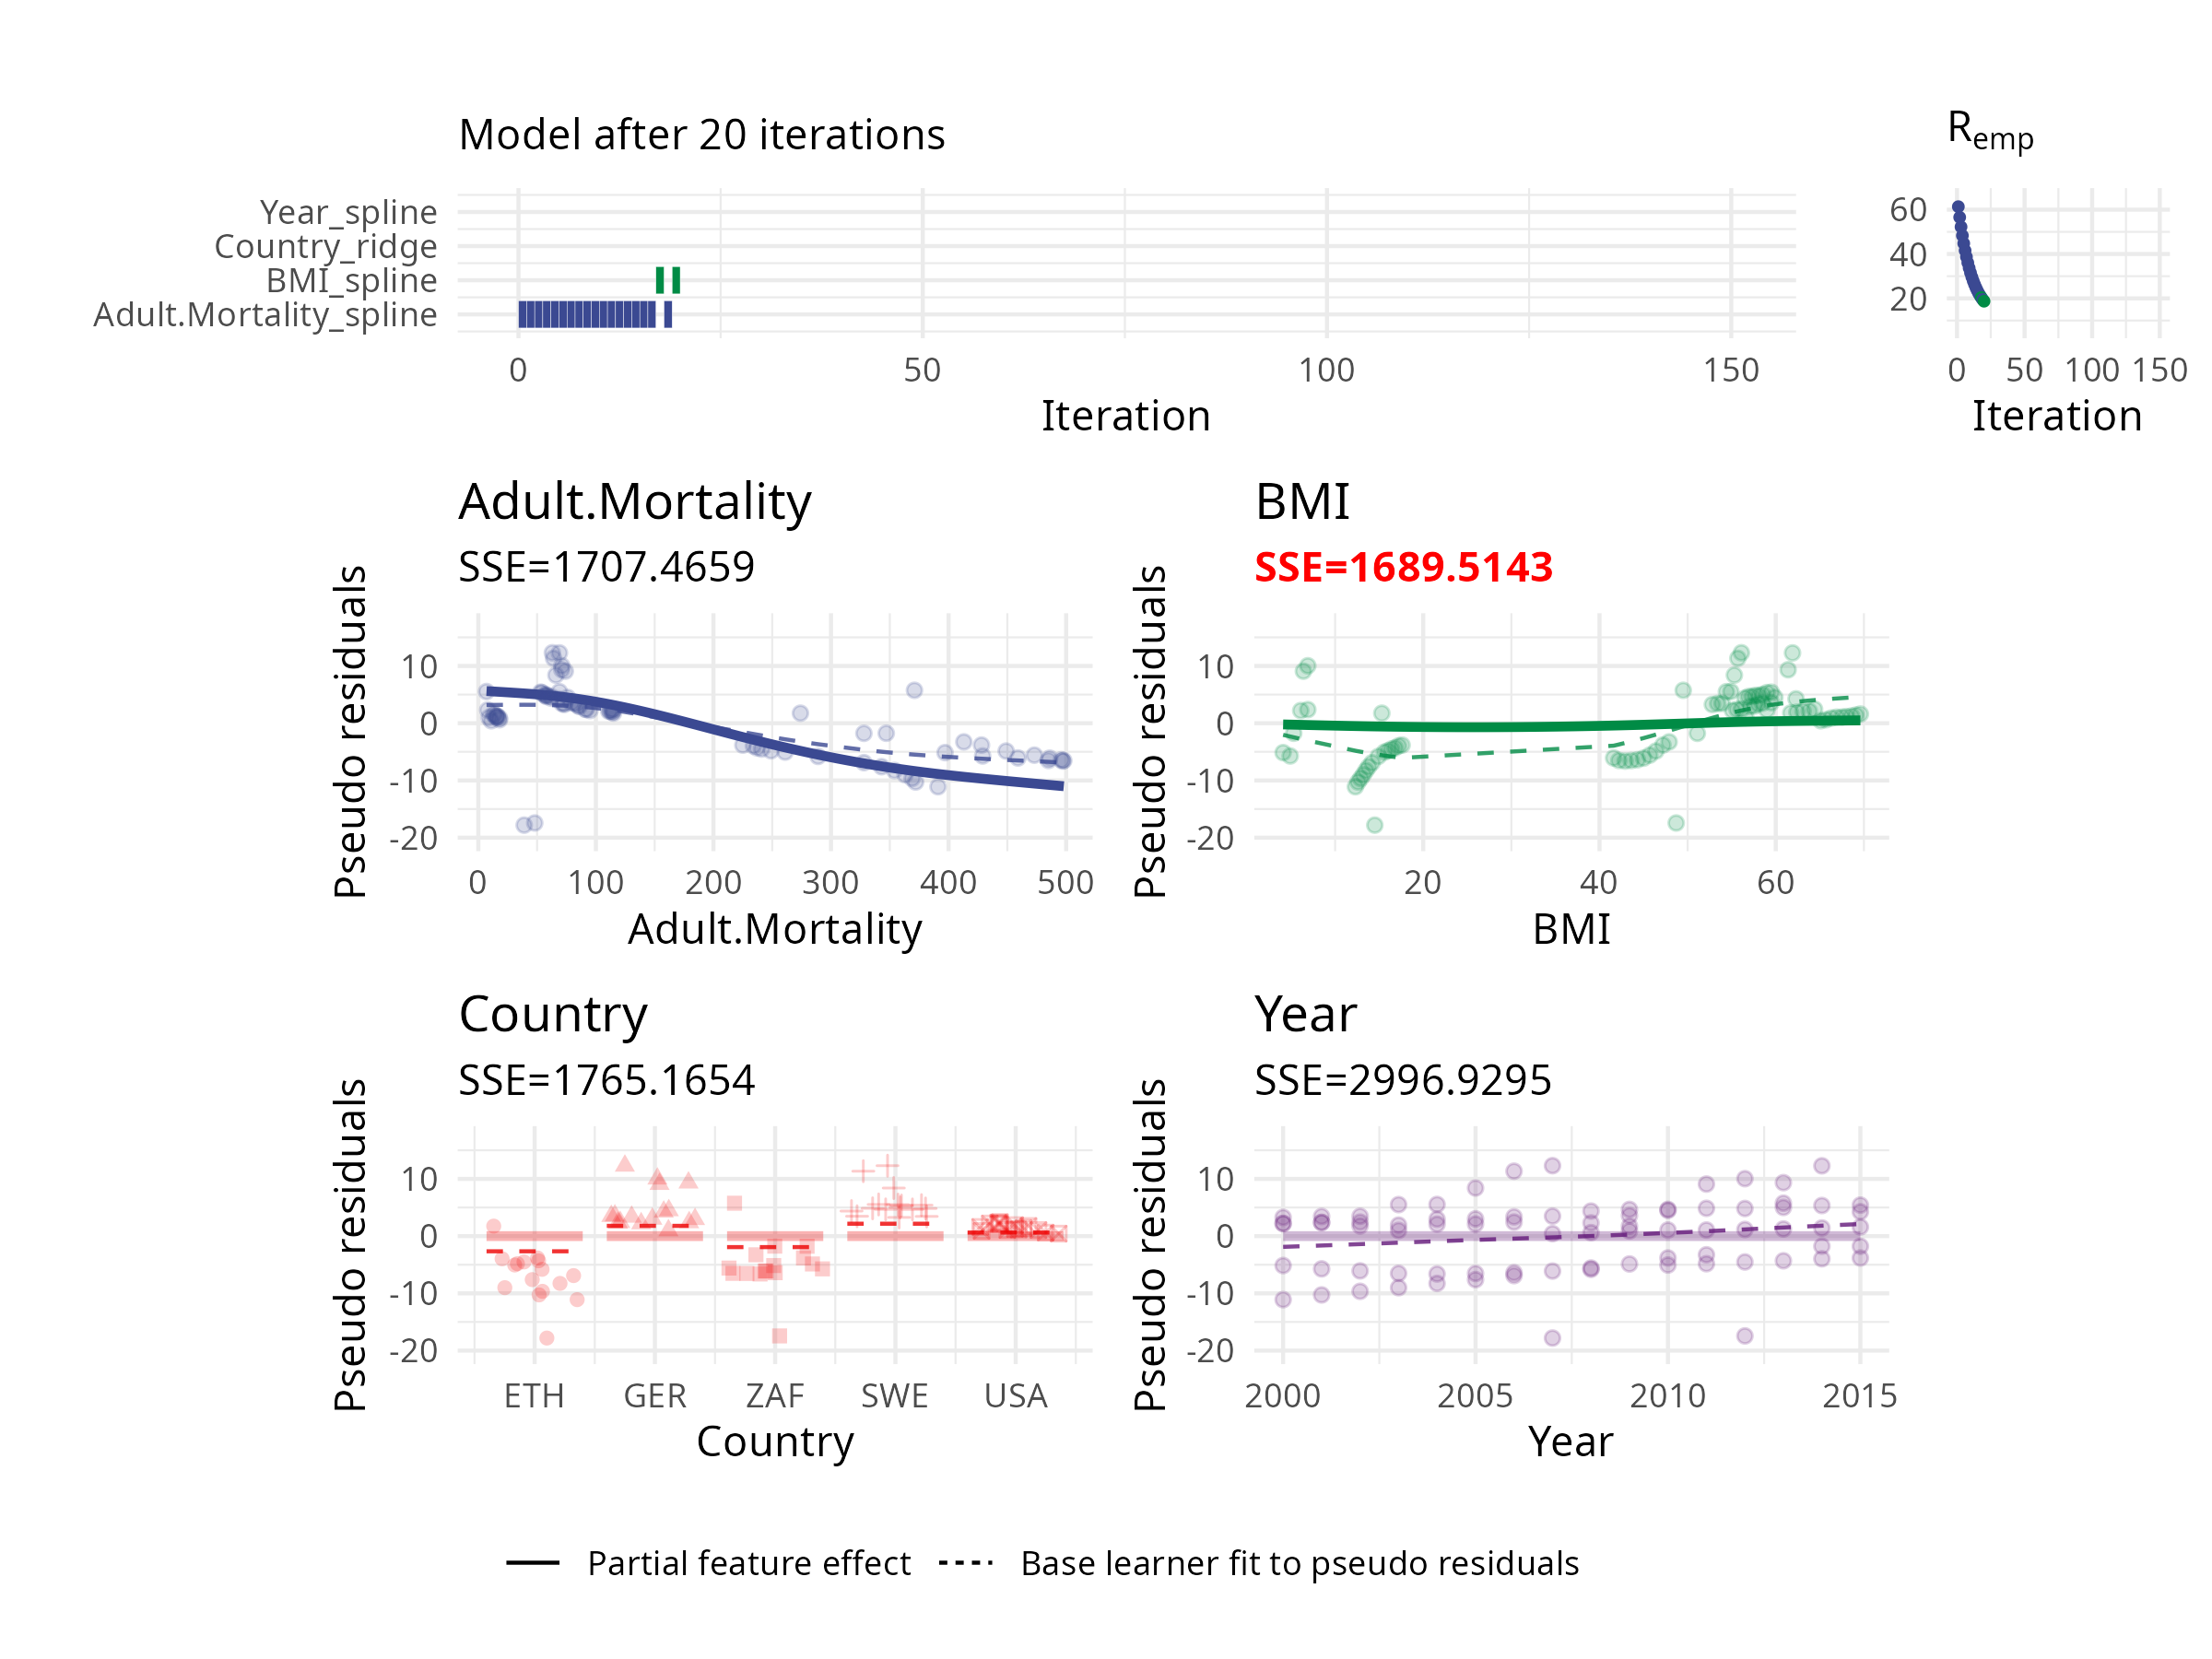
\includegraphics[width=\textwidth]{figure/cwb-anim-nl/fig-iter-0020.png}
	\end{figure}
	\addtocounter{framenumber}{-1}
\end{frame}


\begin{frame}{Example: Life expectancy (nonlinear)}
	\begin{figure}
		\centering
		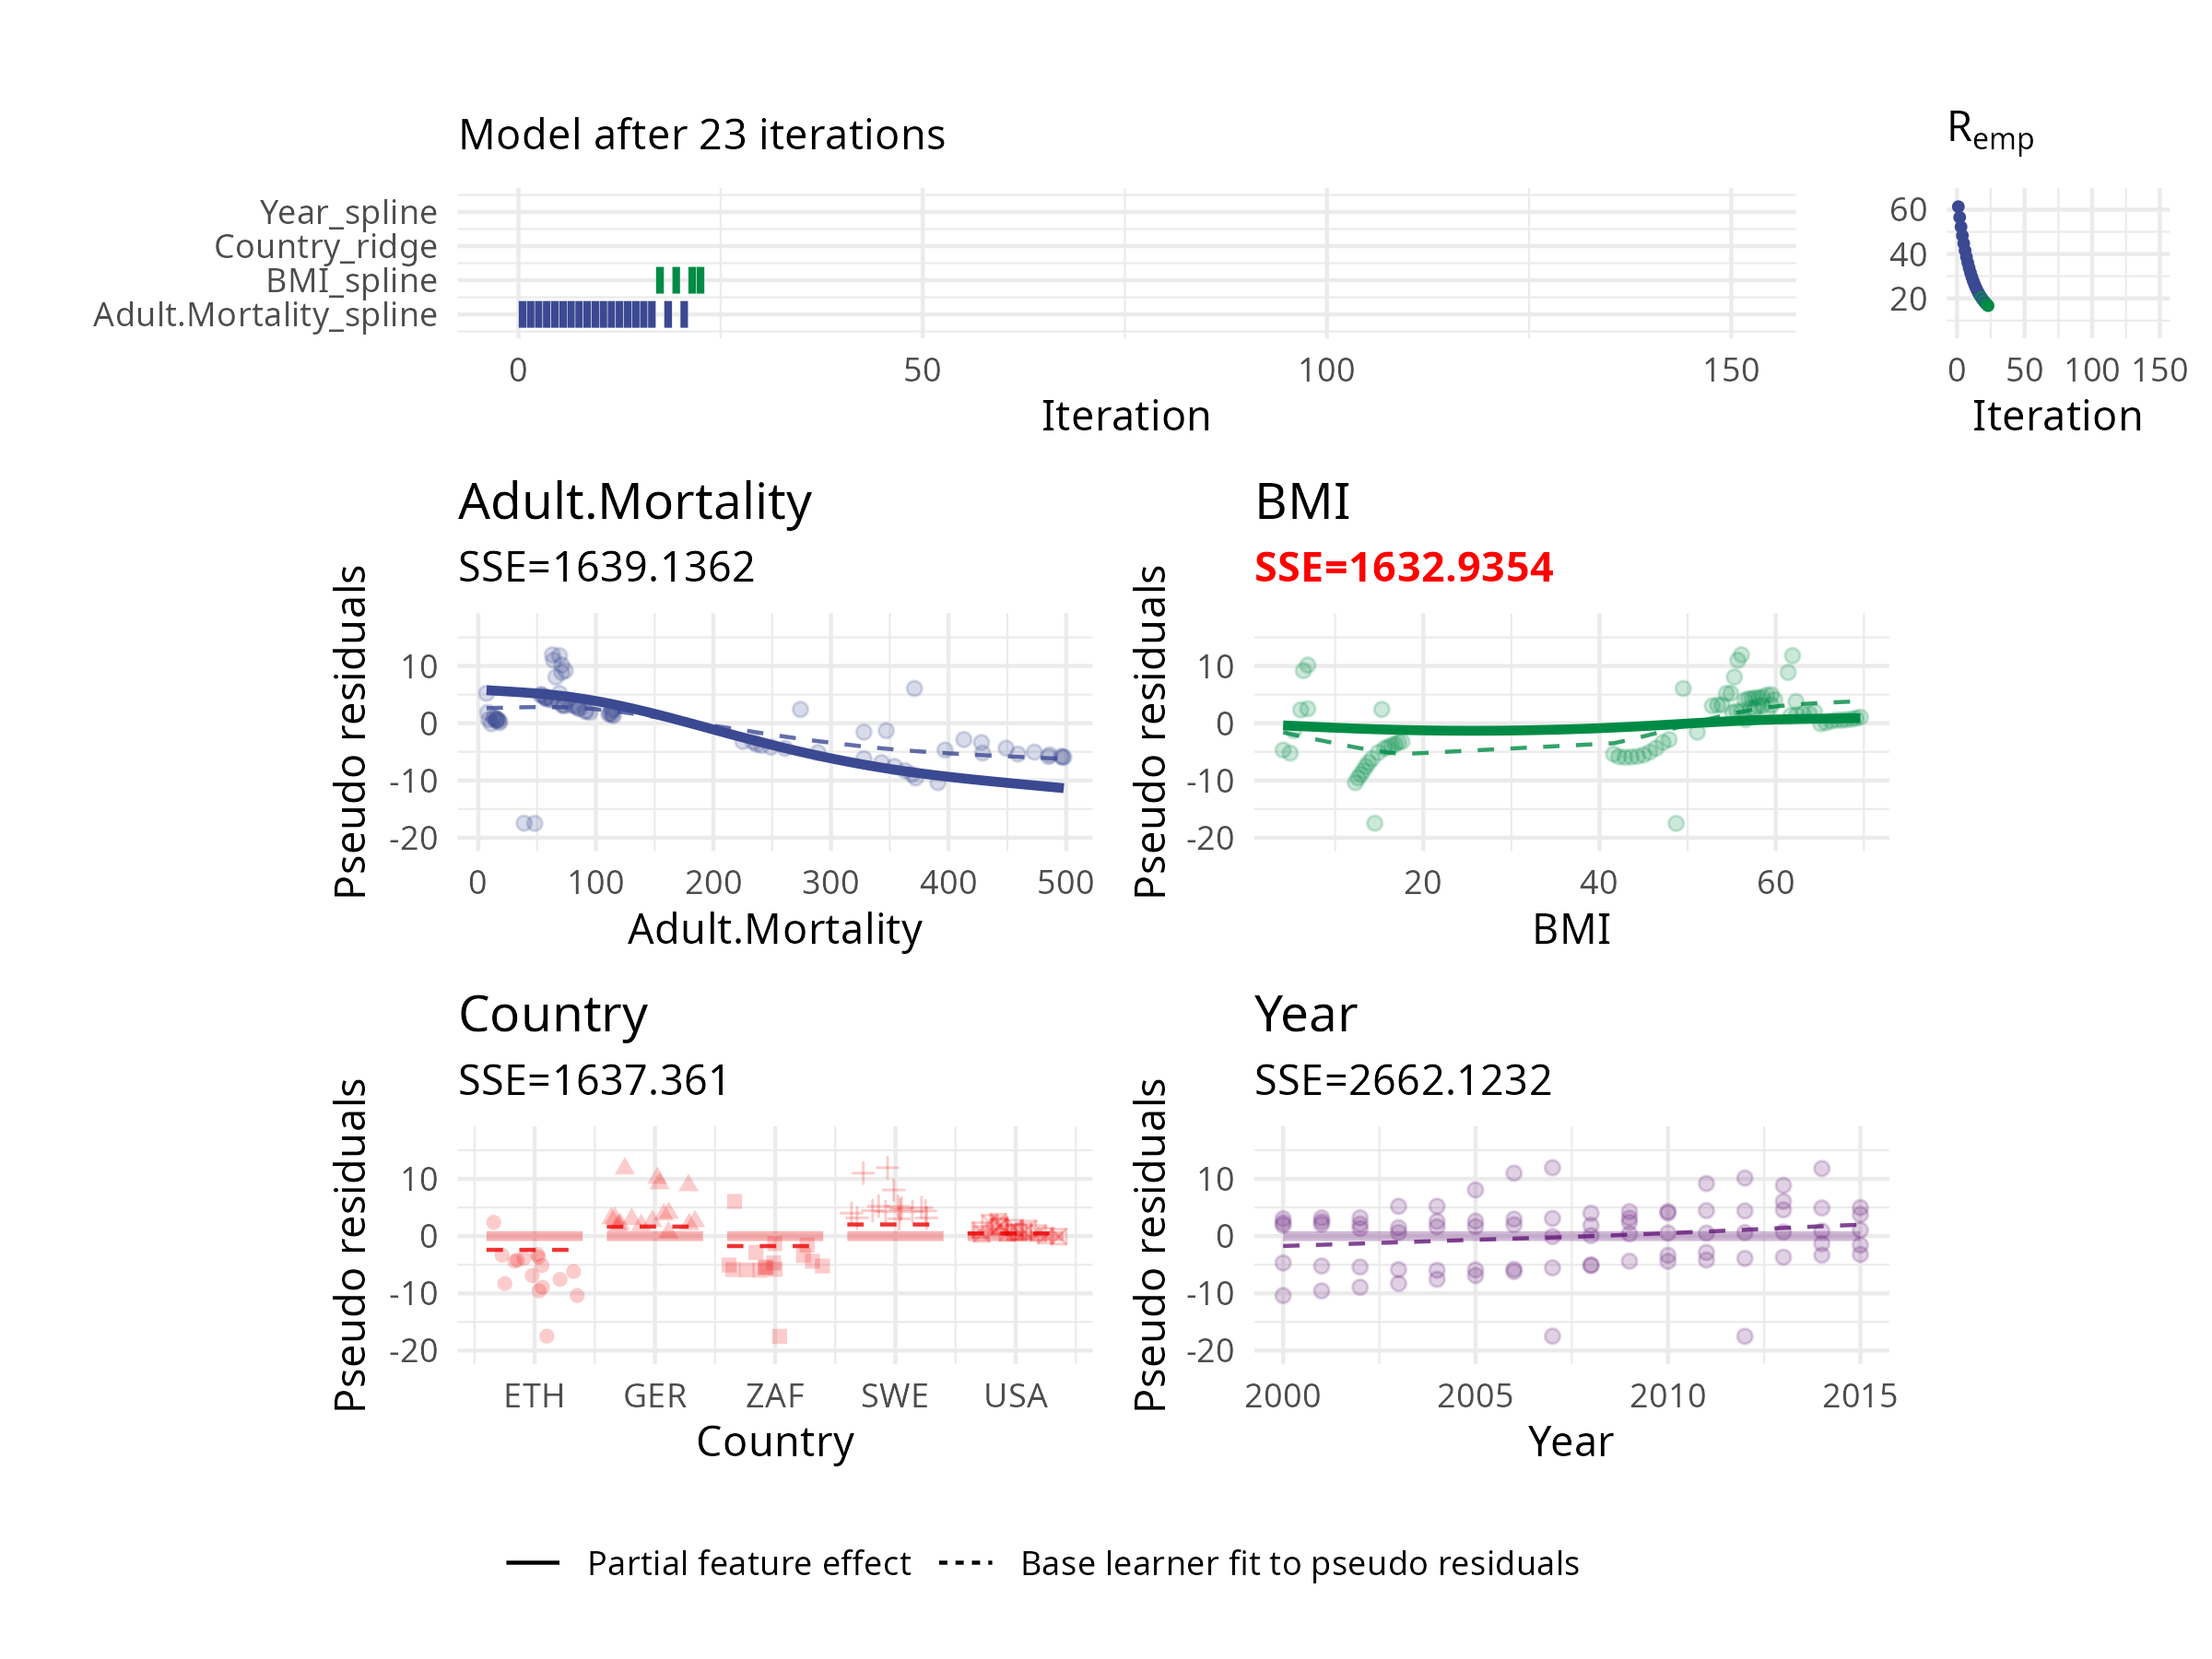
\includegraphics[width=\textwidth]{figure/cwb-anim-nl/fig-iter-0023.png}
	\end{figure}
	\addtocounter{framenumber}{-1}
\end{frame}


\begin{frame}{Example: Life expectancy (nonlinear)}
	\begin{figure}
		\centering
		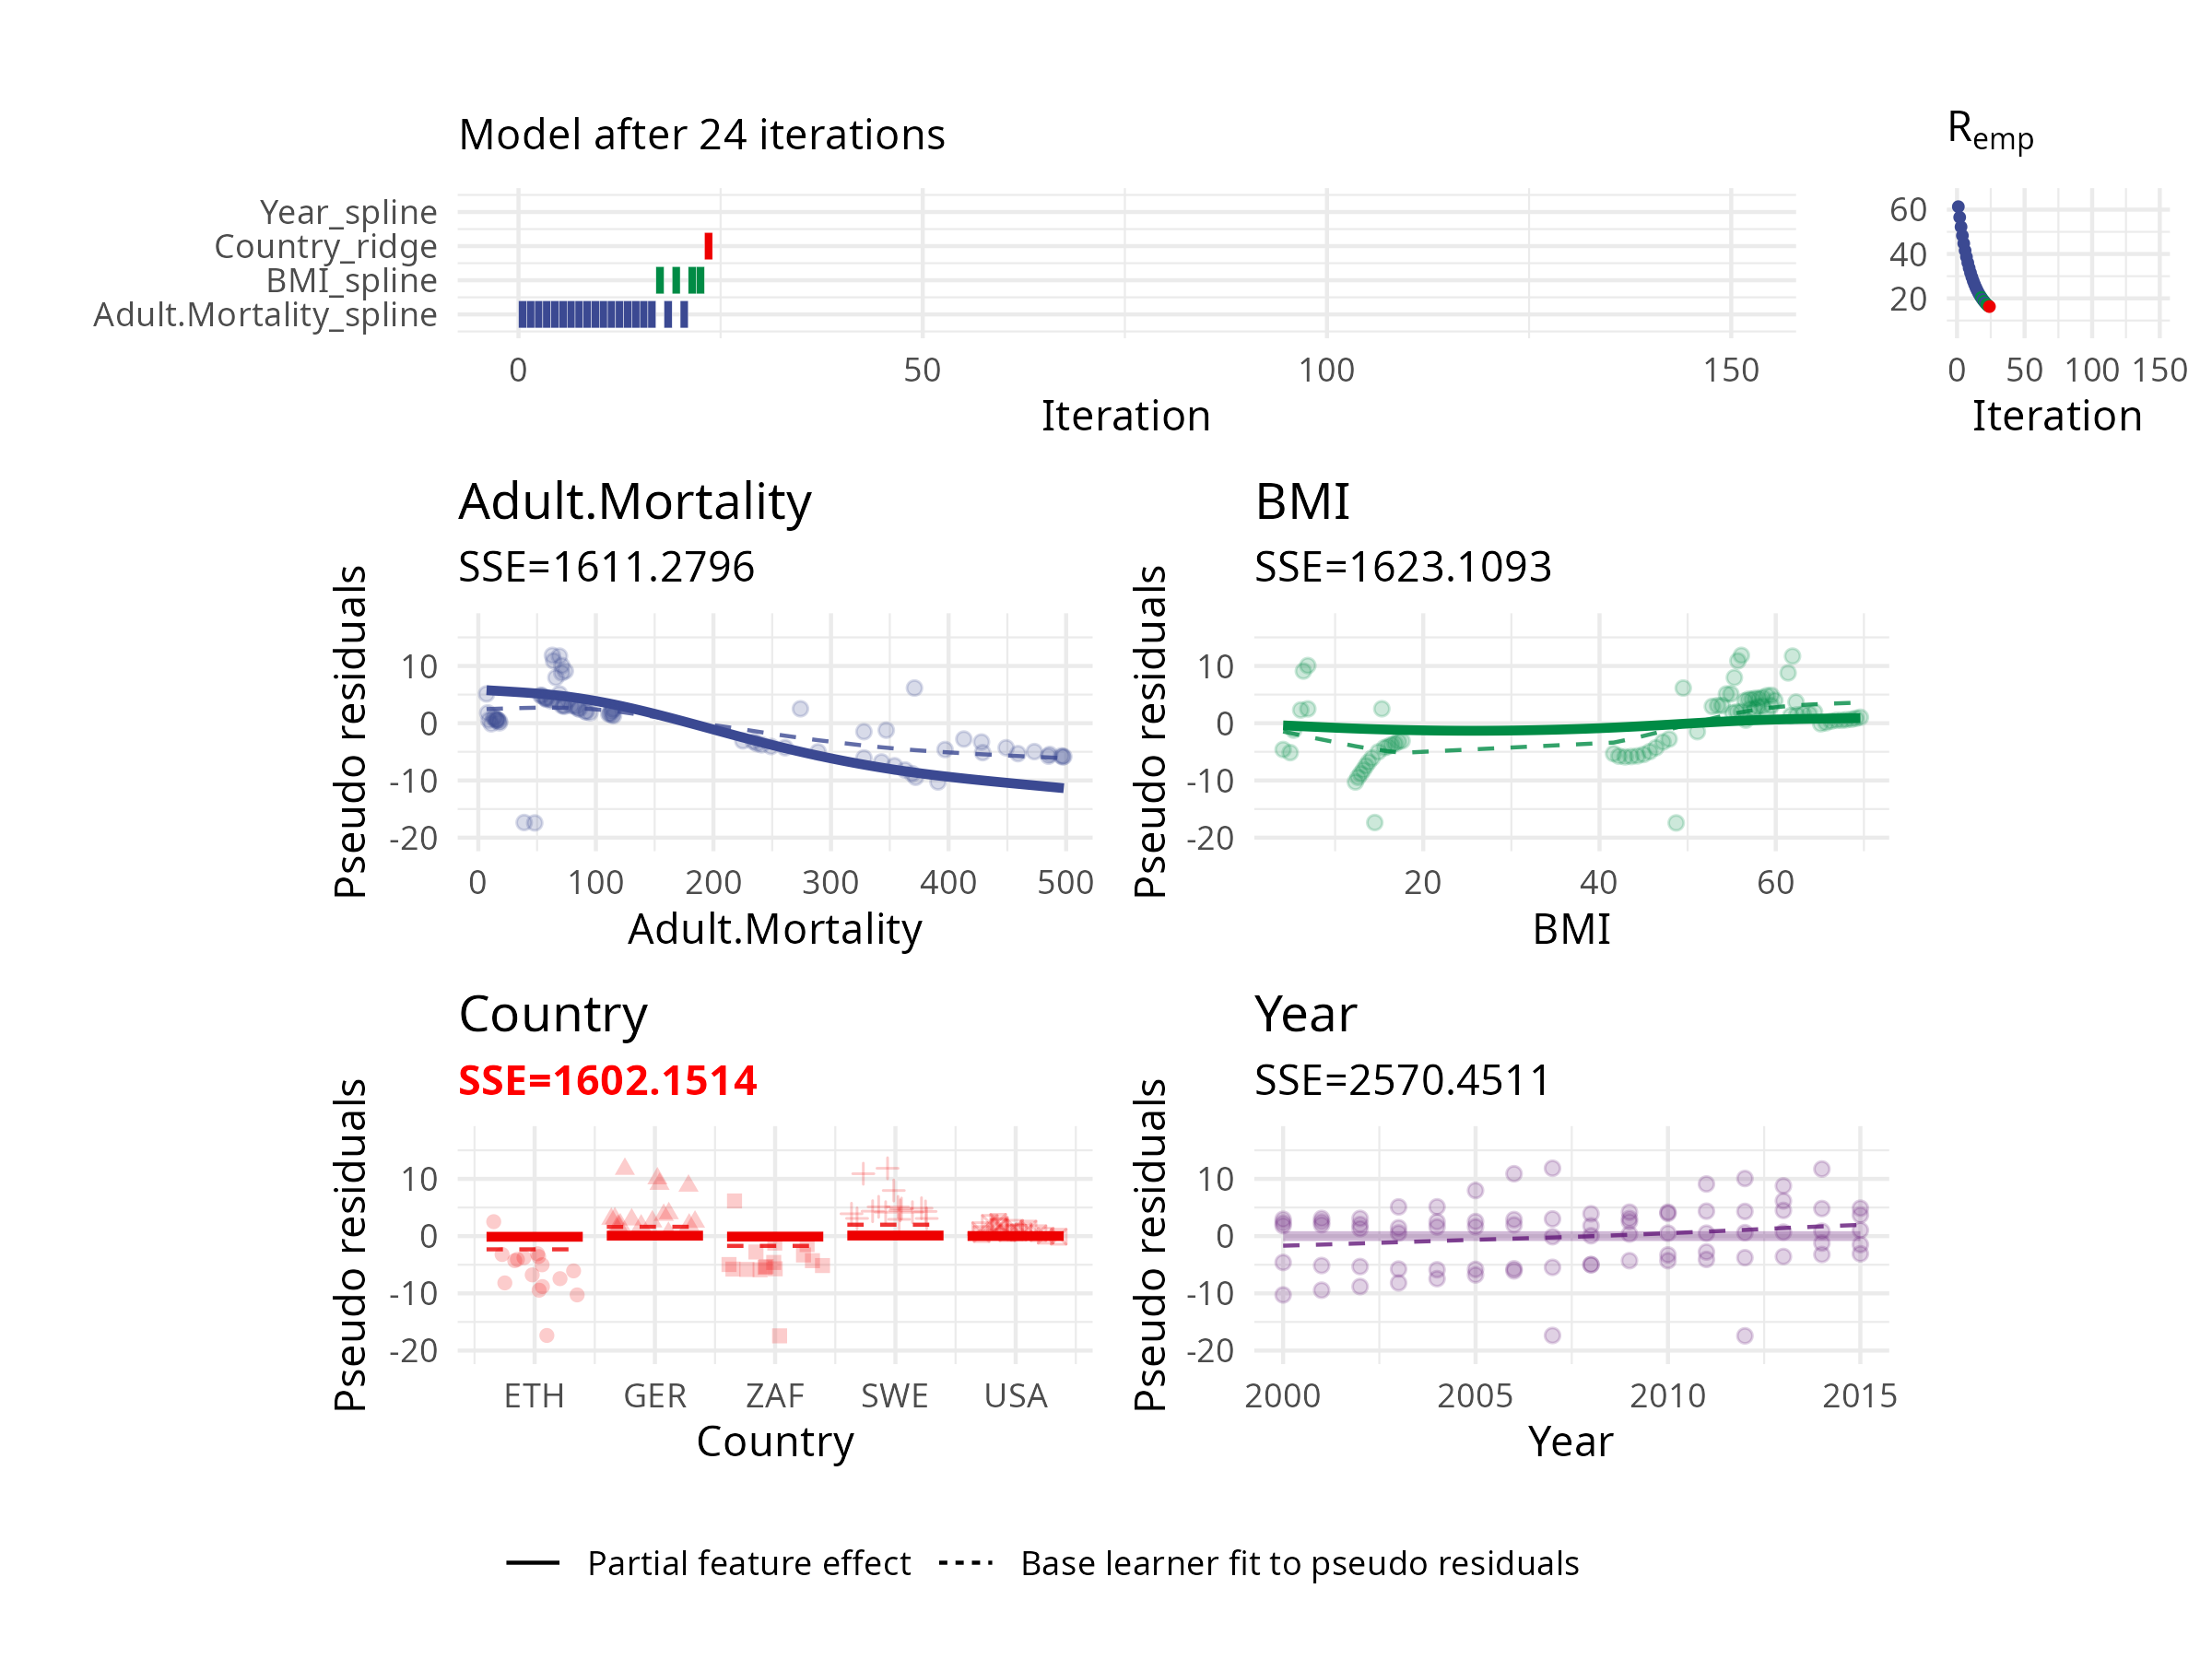
\includegraphics[width=\textwidth]{figure/cwb-anim-nl/fig-iter-0024.png}
	\end{figure}
	\addtocounter{framenumber}{-1}
\end{frame}


\begin{frame}{Example: Life expectancy (nonlinear)}
	\begin{figure}
		\centering
		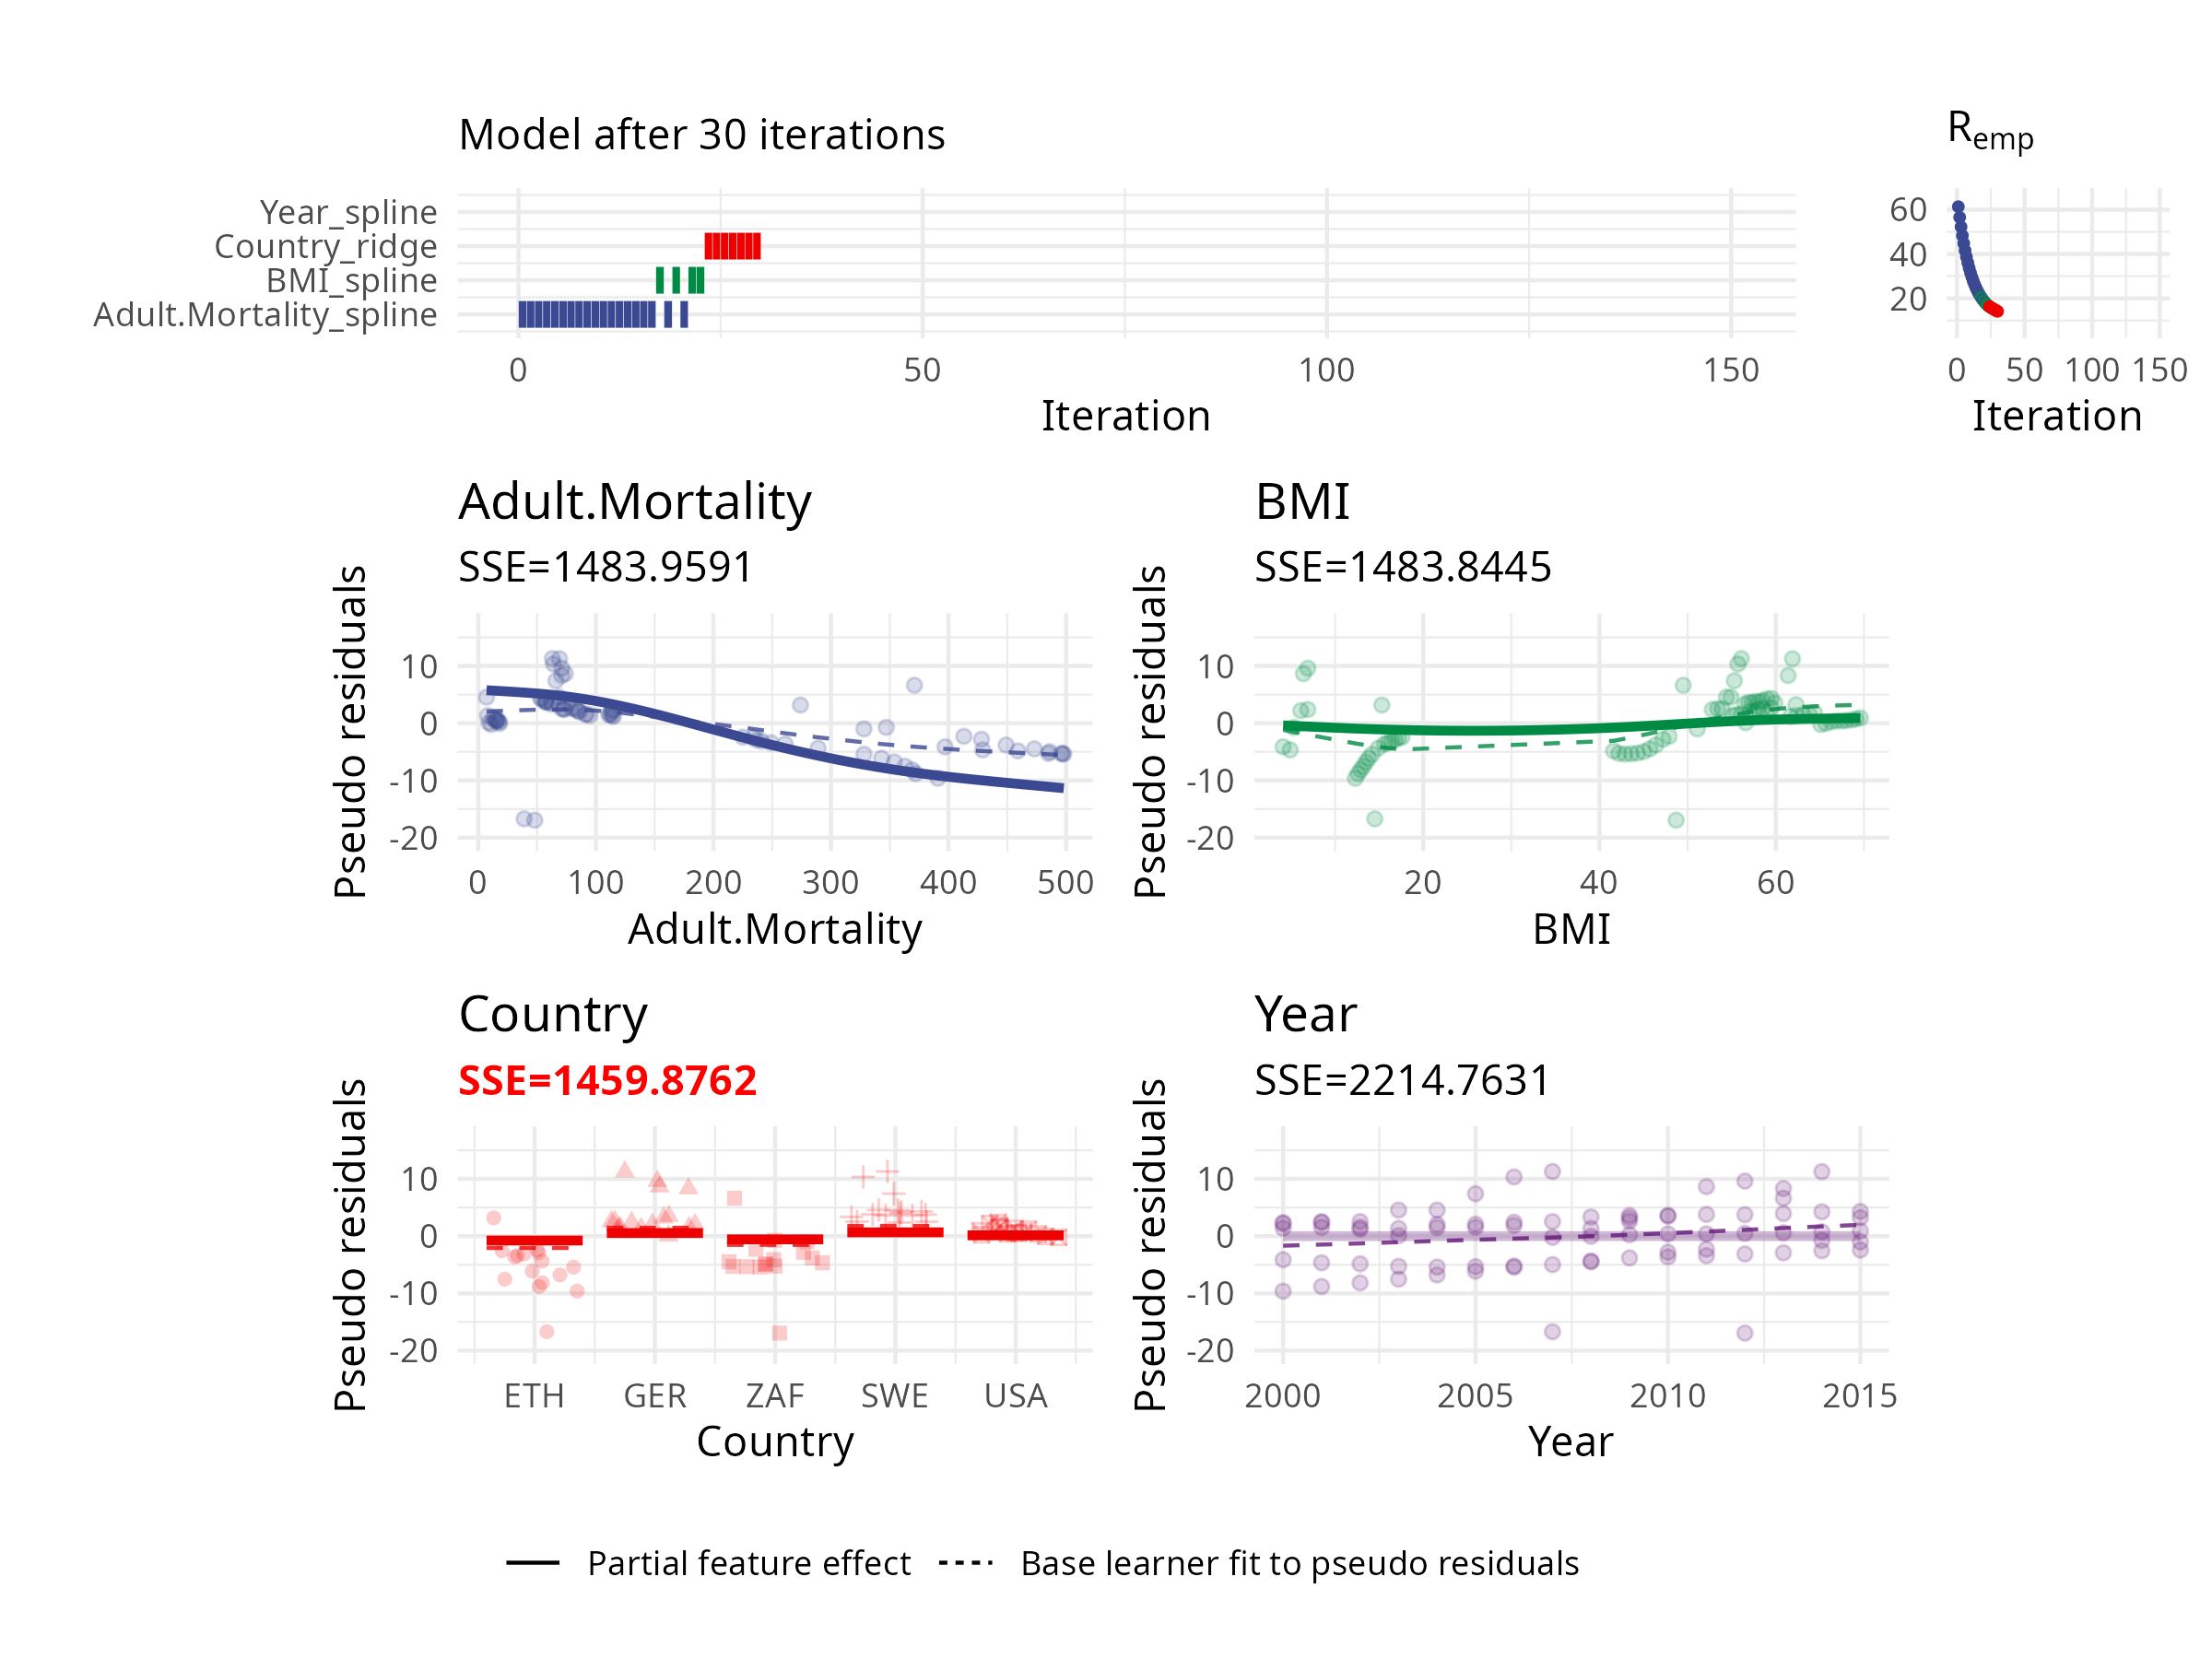
\includegraphics[width=\textwidth]{figure/cwb-anim-nl/fig-iter-0030.png}
	\end{figure}
	\addtocounter{framenumber}{-1}
\end{frame}


\begin{frame}{Example: Life expectancy (nonlinear)}
	\begin{figure}
		\centering
		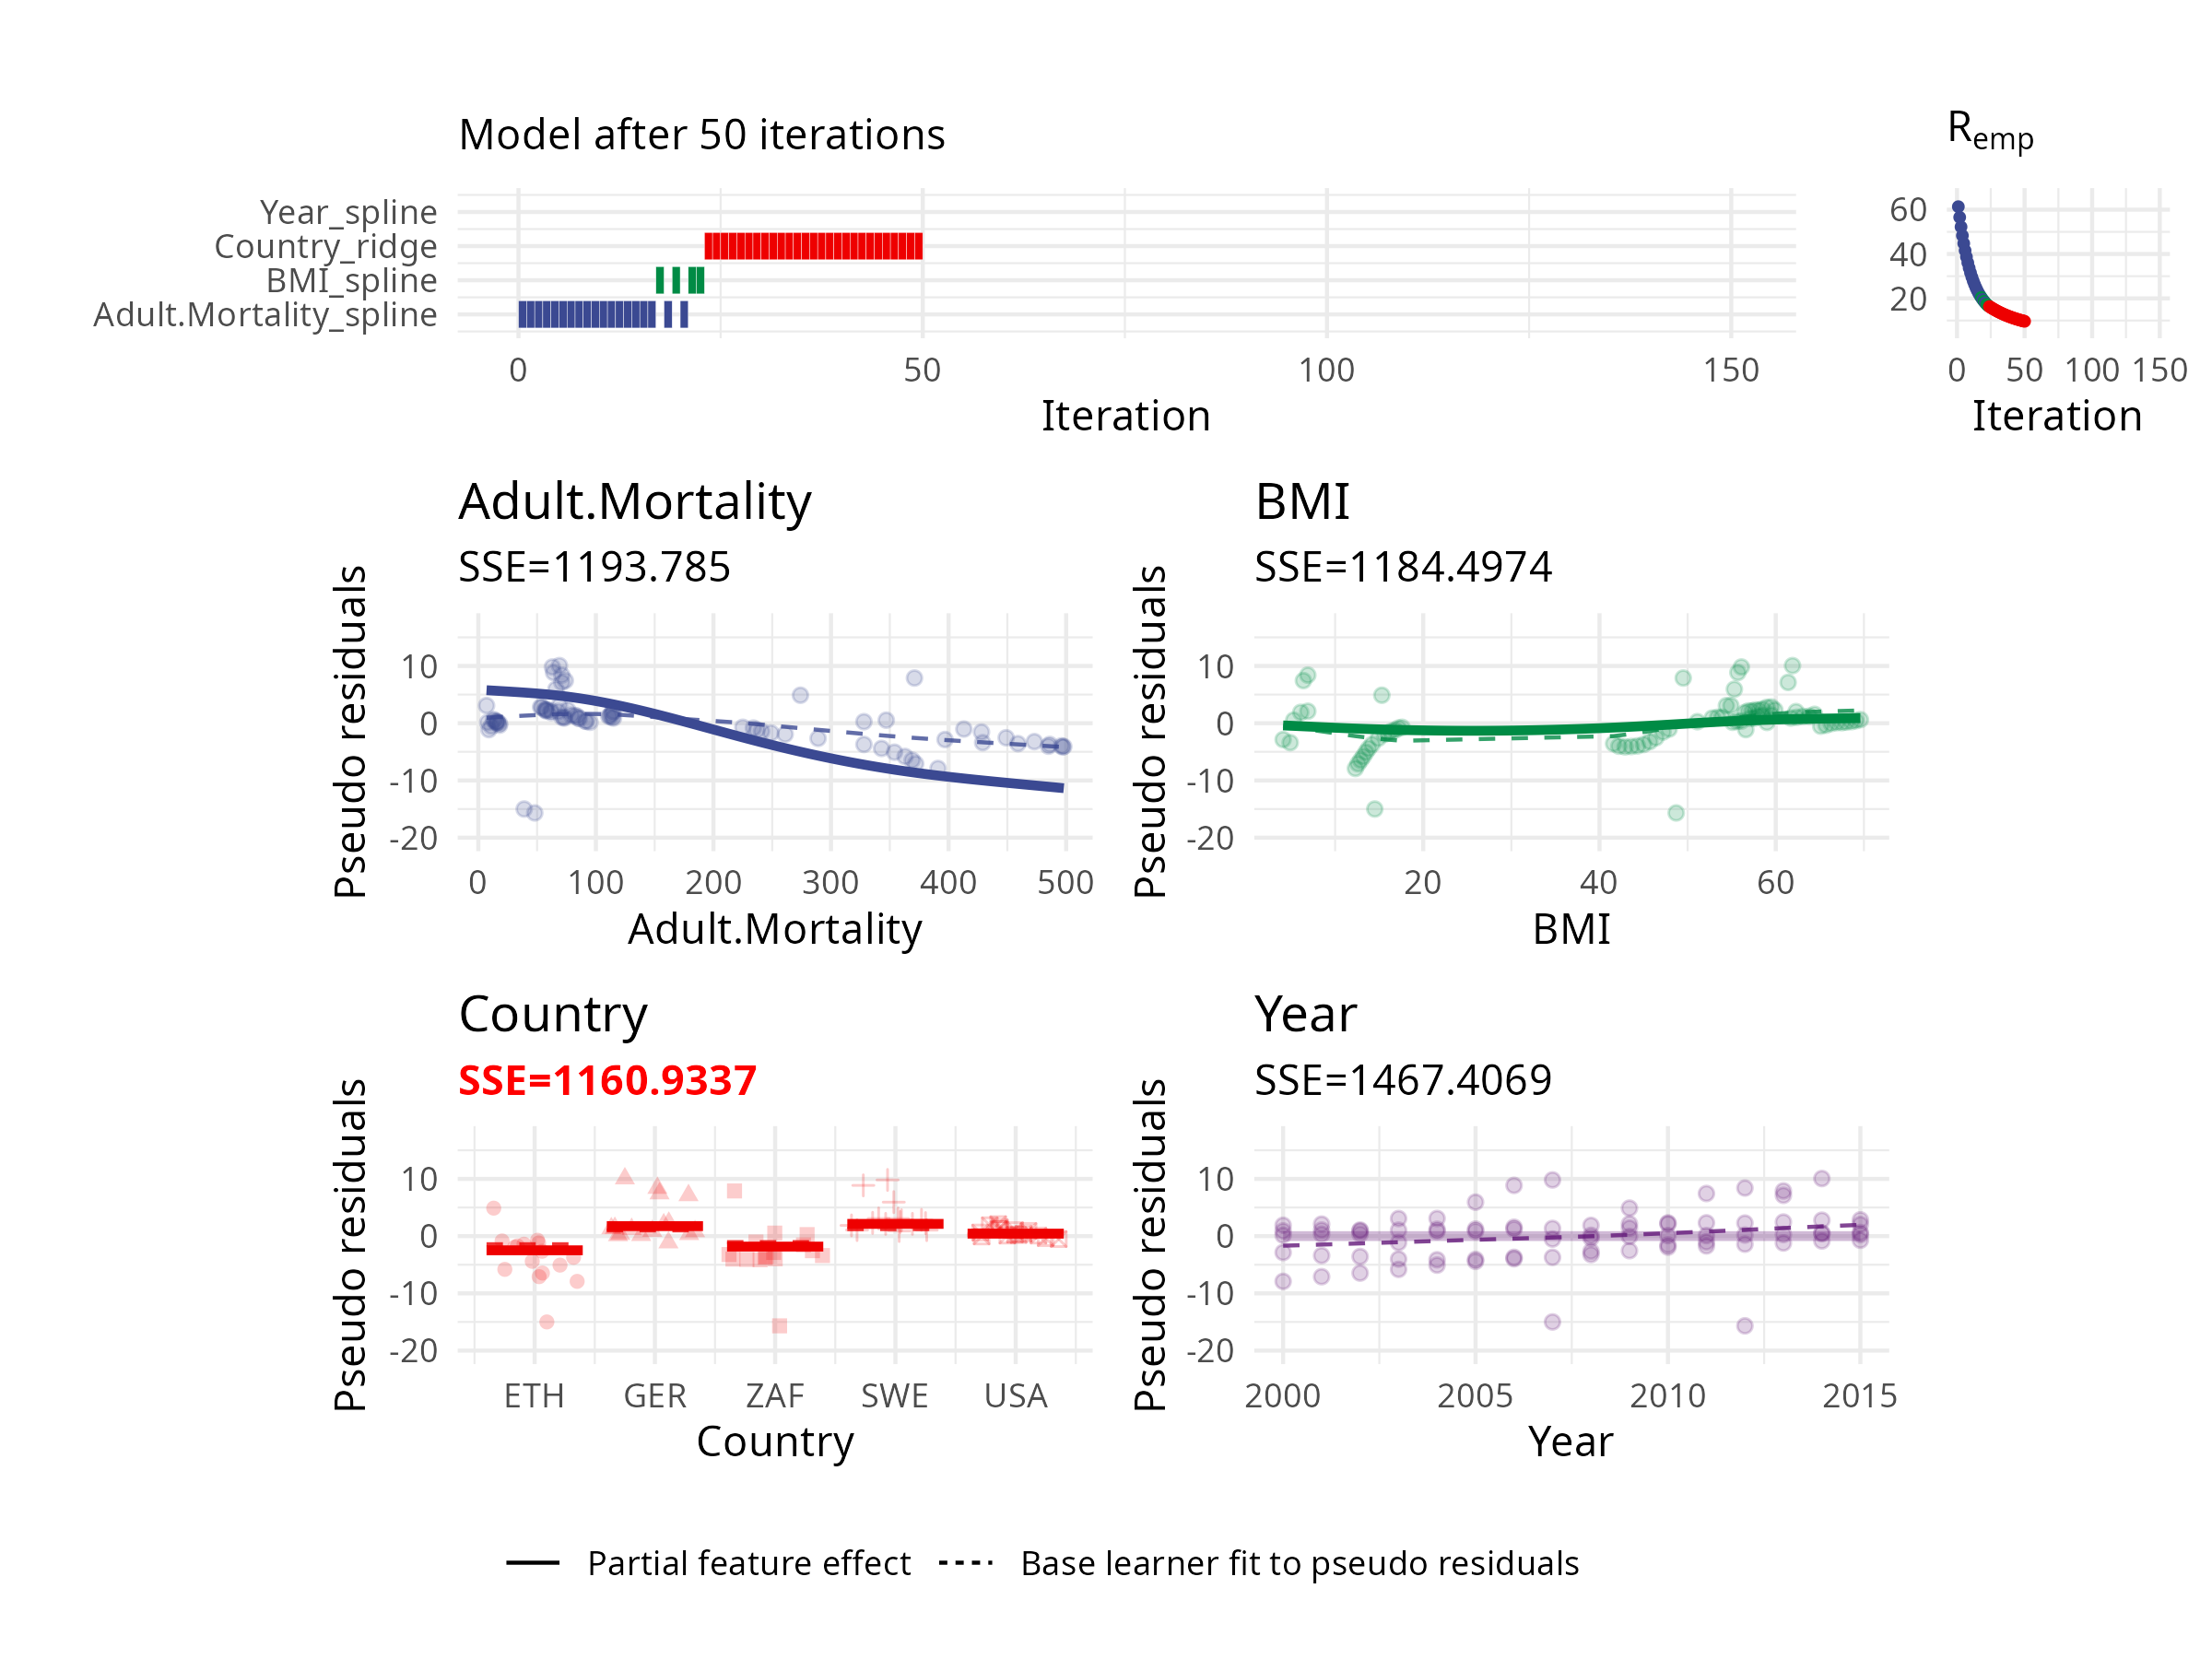
\includegraphics[width=\textwidth]{figure/cwb-anim-nl/fig-iter-0050.png}
	\end{figure}
	\addtocounter{framenumber}{-1}
\end{frame}


\begin{frame}{Example: Life expectancy (nonlinear)}
	\begin{figure}
		\centering
		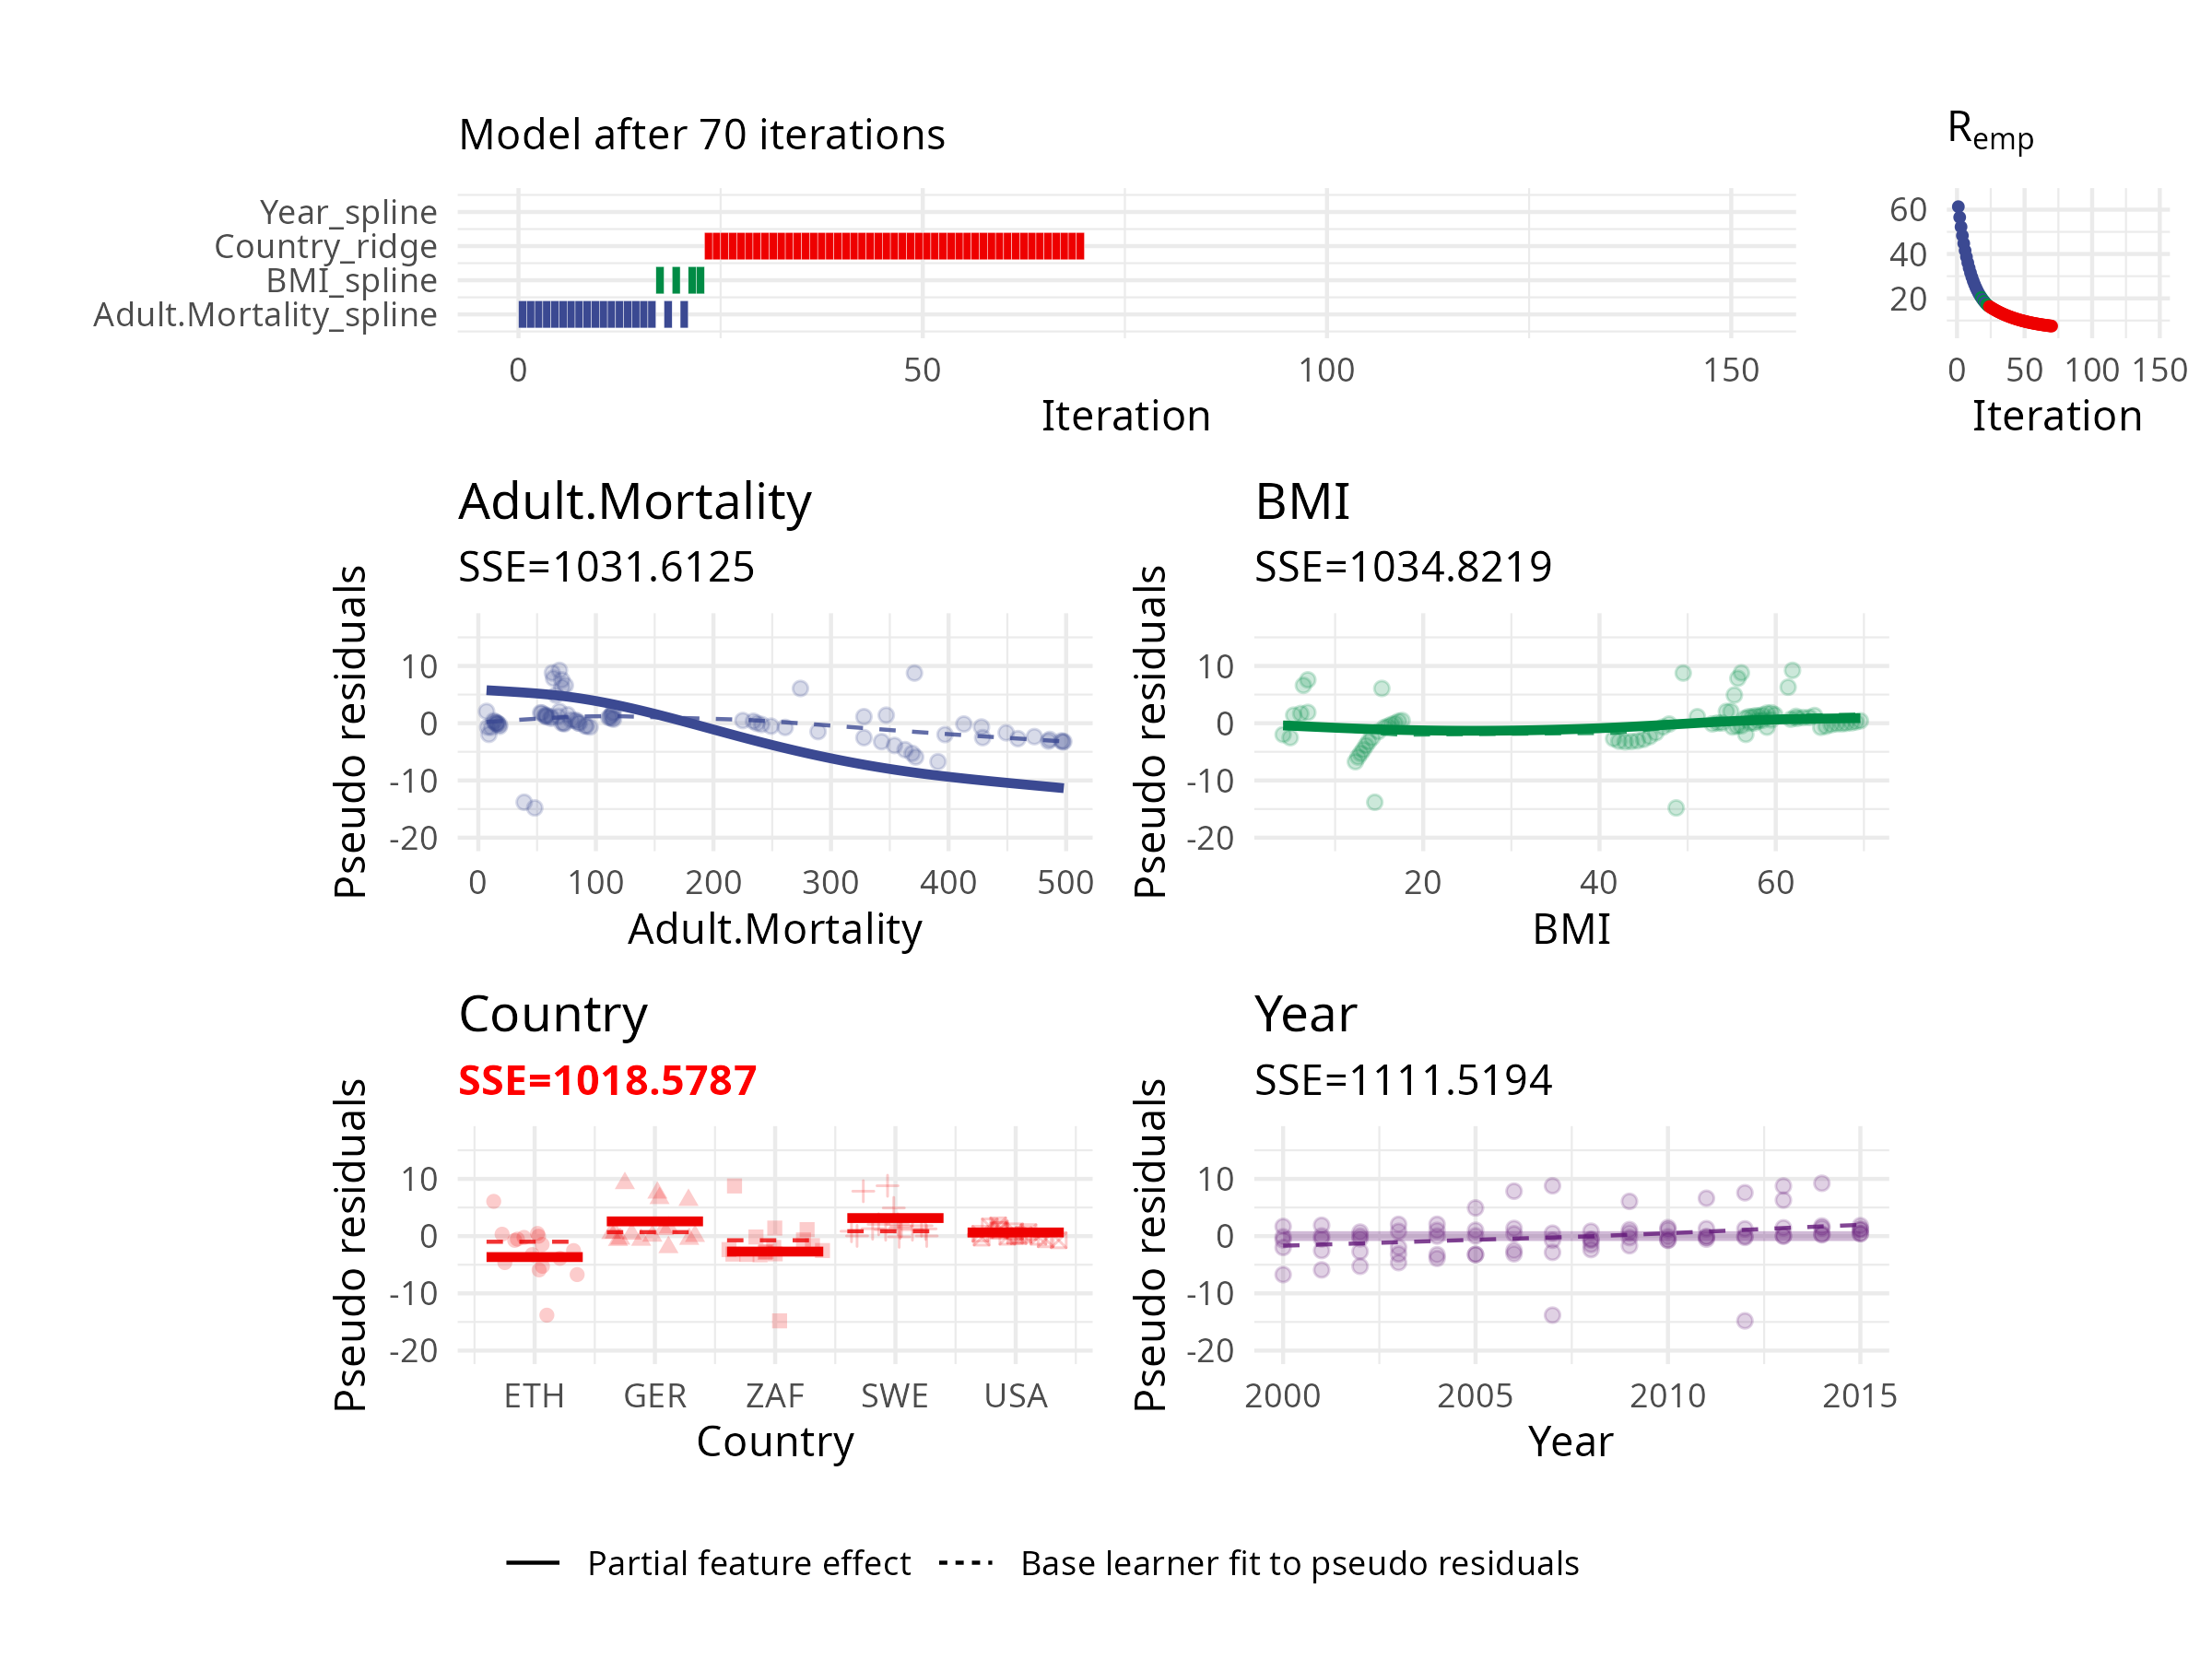
\includegraphics[width=\textwidth]{figure/cwb-anim-nl/fig-iter-0070.png}
	\end{figure}
	\addtocounter{framenumber}{-1}
\end{frame}


\begin{frame}{Example: Life expectancy (nonlinear)}
	\begin{figure}
		\centering
		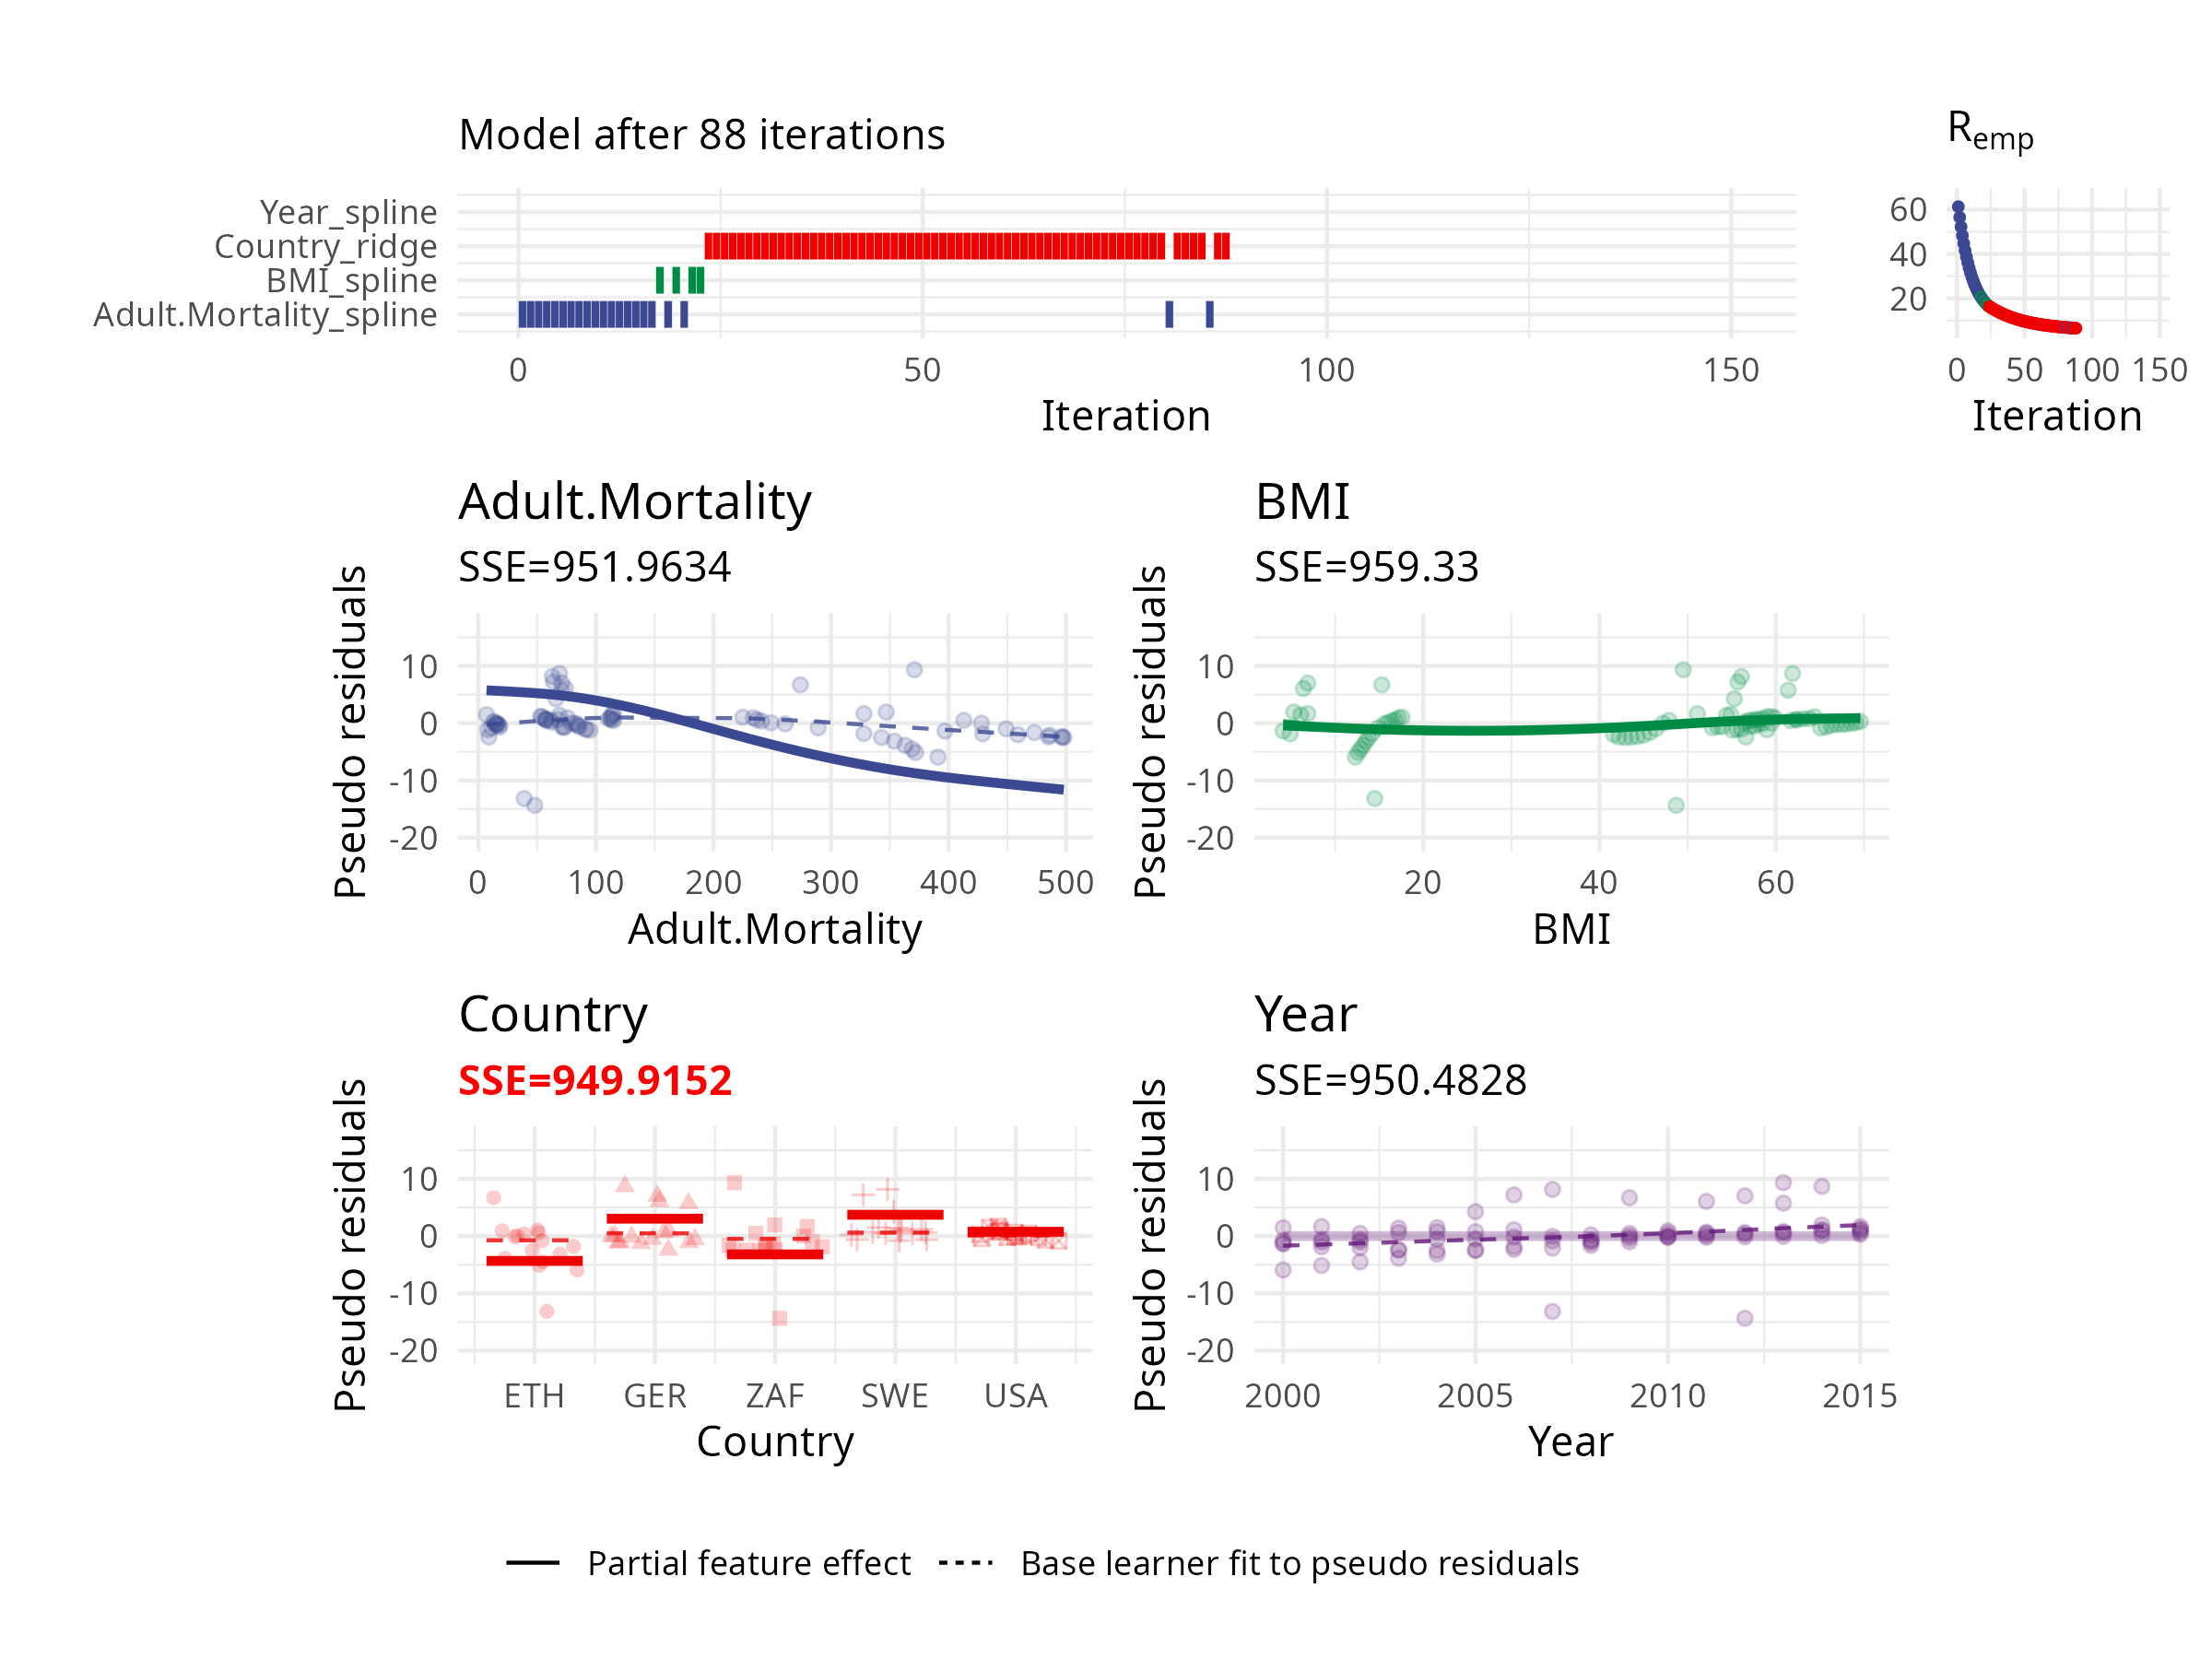
\includegraphics[width=\textwidth]{figure/cwb-anim-nl/fig-iter-0088.png}
	\end{figure}
	\addtocounter{framenumber}{-1}
\end{frame}


\begin{frame}{Example: Life expectancy (nonlinear)}
	\begin{figure}
		\centering
		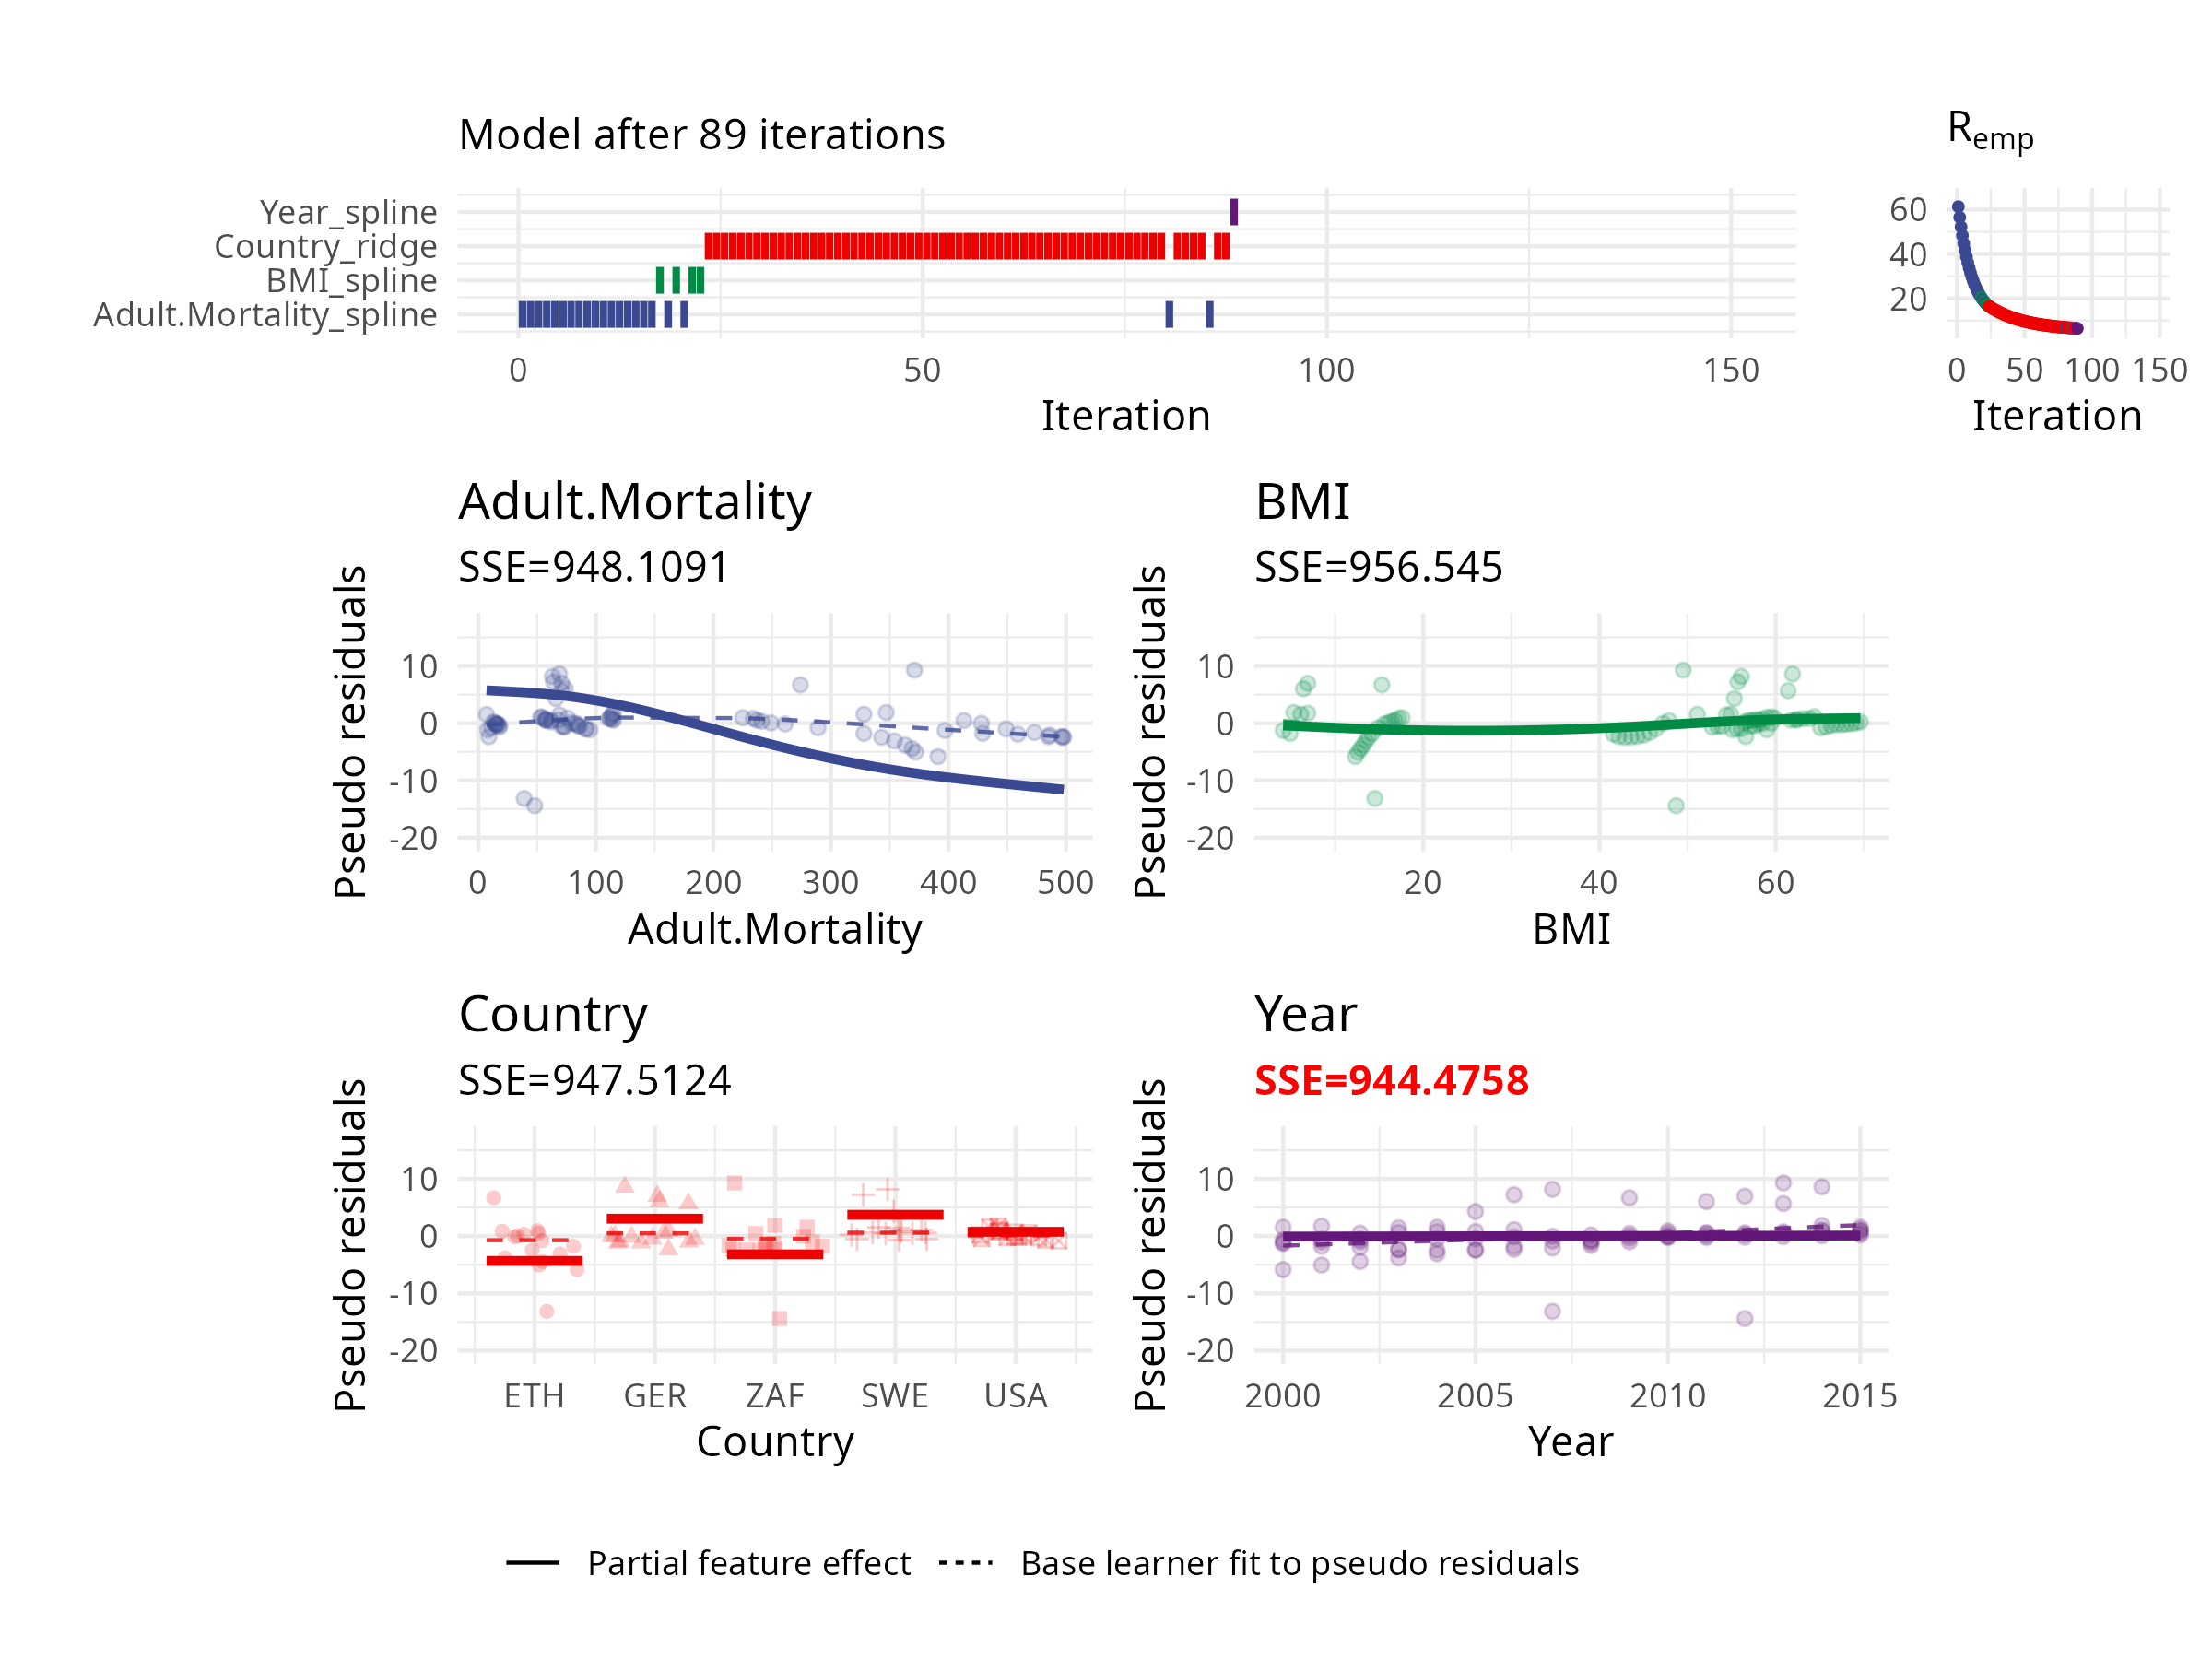
\includegraphics[width=\textwidth]{figure/cwb-anim-nl/fig-iter-0089.png}
	\end{figure}
	\addtocounter{framenumber}{-1}
\end{frame}


\begin{frame}{Example: Life expectancy (nonlinear)}
	\begin{figure}
		\centering
		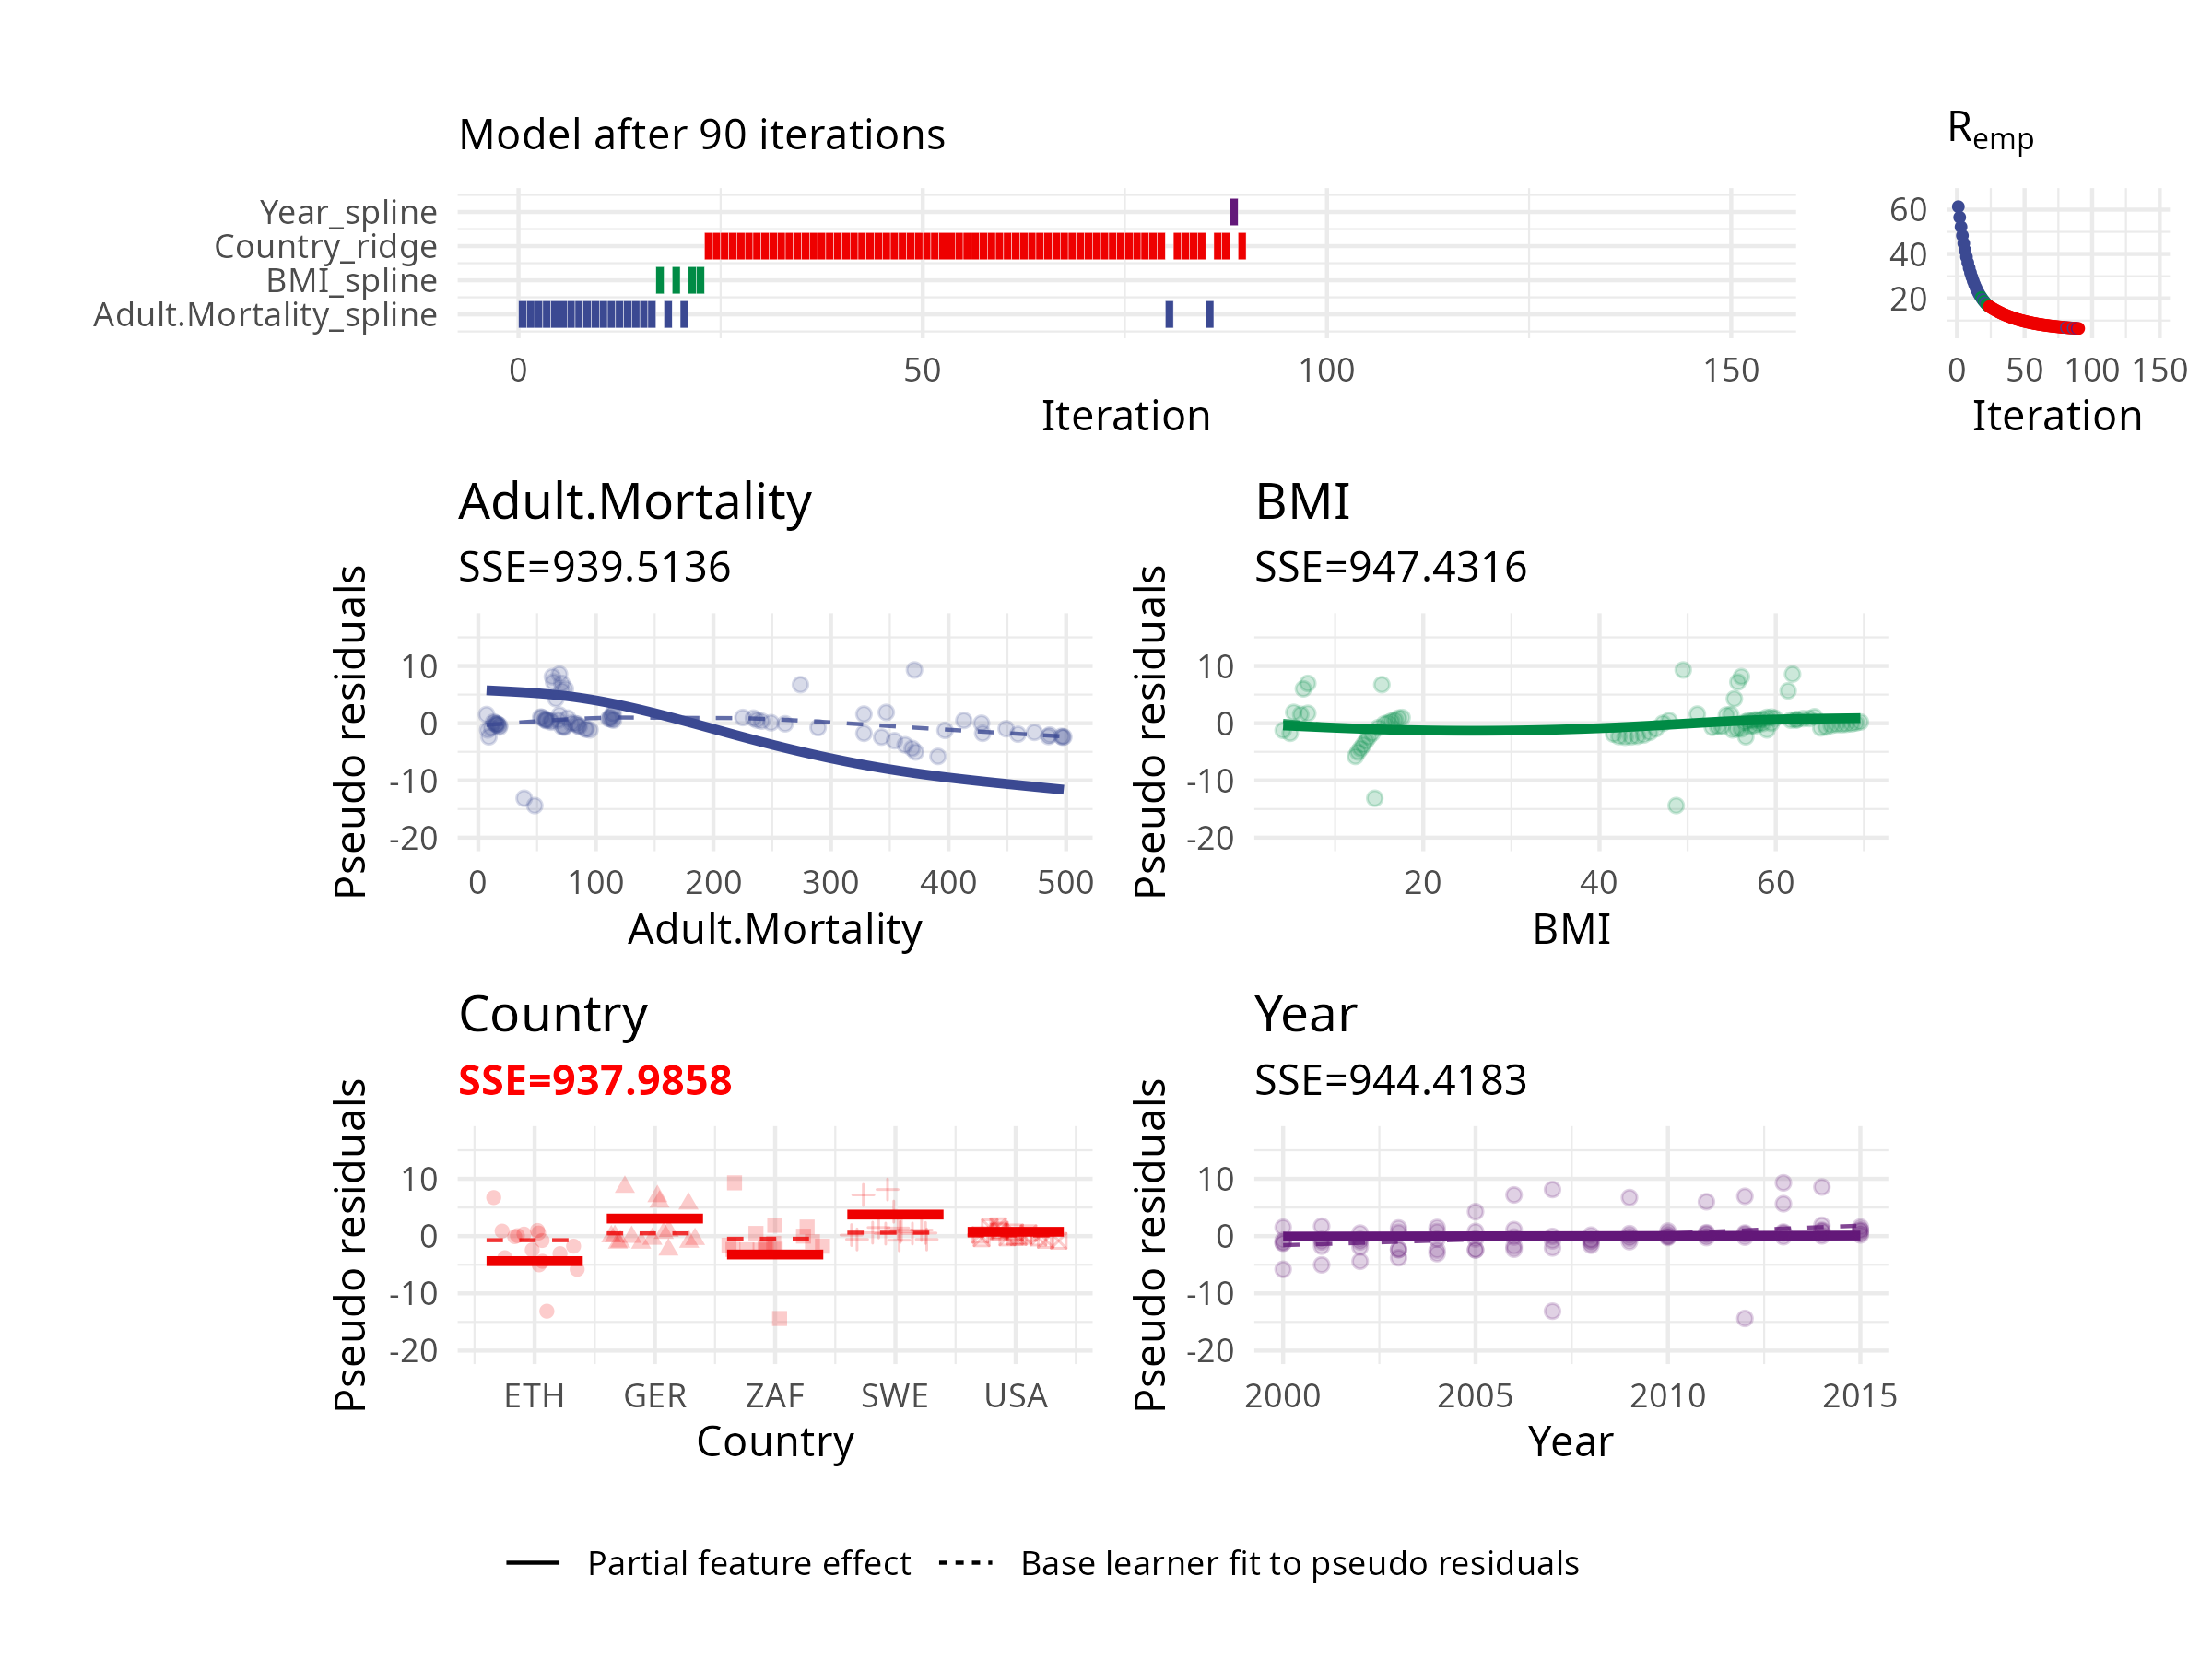
\includegraphics[width=\textwidth]{figure/cwb-anim-nl/fig-iter-0090.png}
	\end{figure}
	\addtocounter{framenumber}{-1}
\end{frame}


\begin{frame}{Example: Life expectancy (nonlinear)}
	\begin{figure}
		\centering
		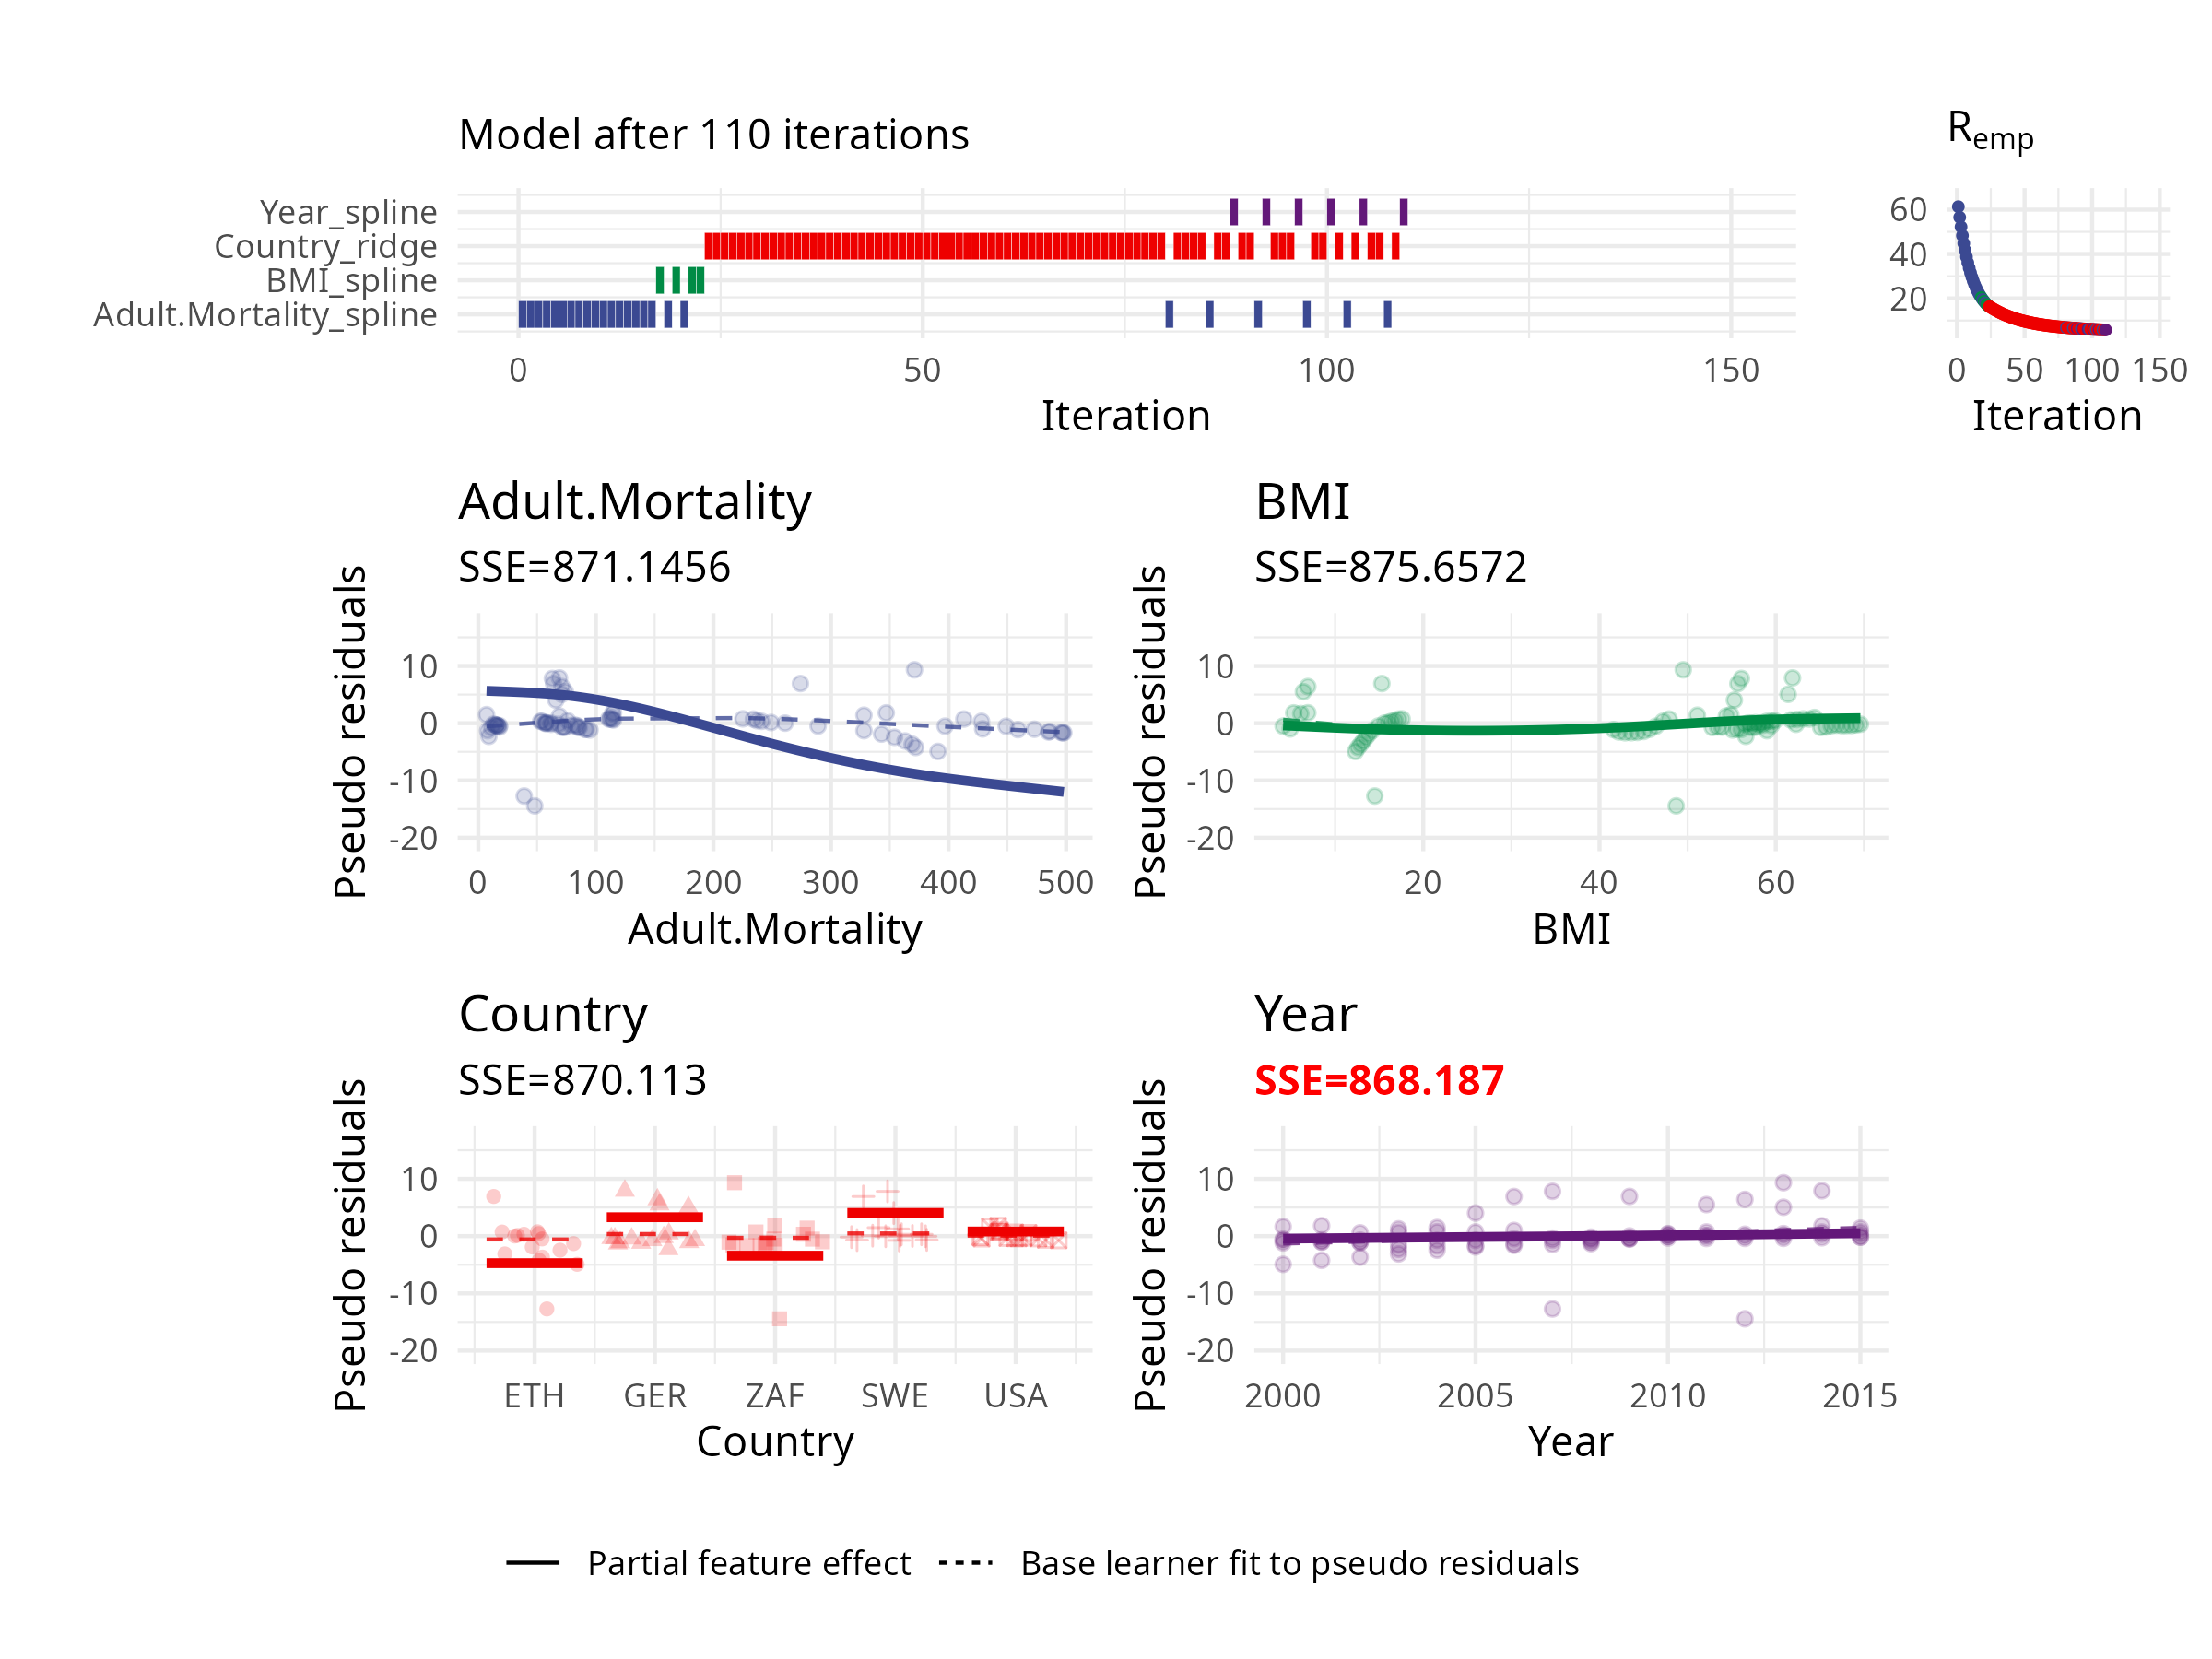
\includegraphics[width=\textwidth]{figure/cwb-anim-nl/fig-iter-0110.png}
	\end{figure}
	\addtocounter{framenumber}{-1}
\end{frame}


\begin{frame}{Example: Life expectancy (nonlinear)}
	\begin{figure}
		\centering
		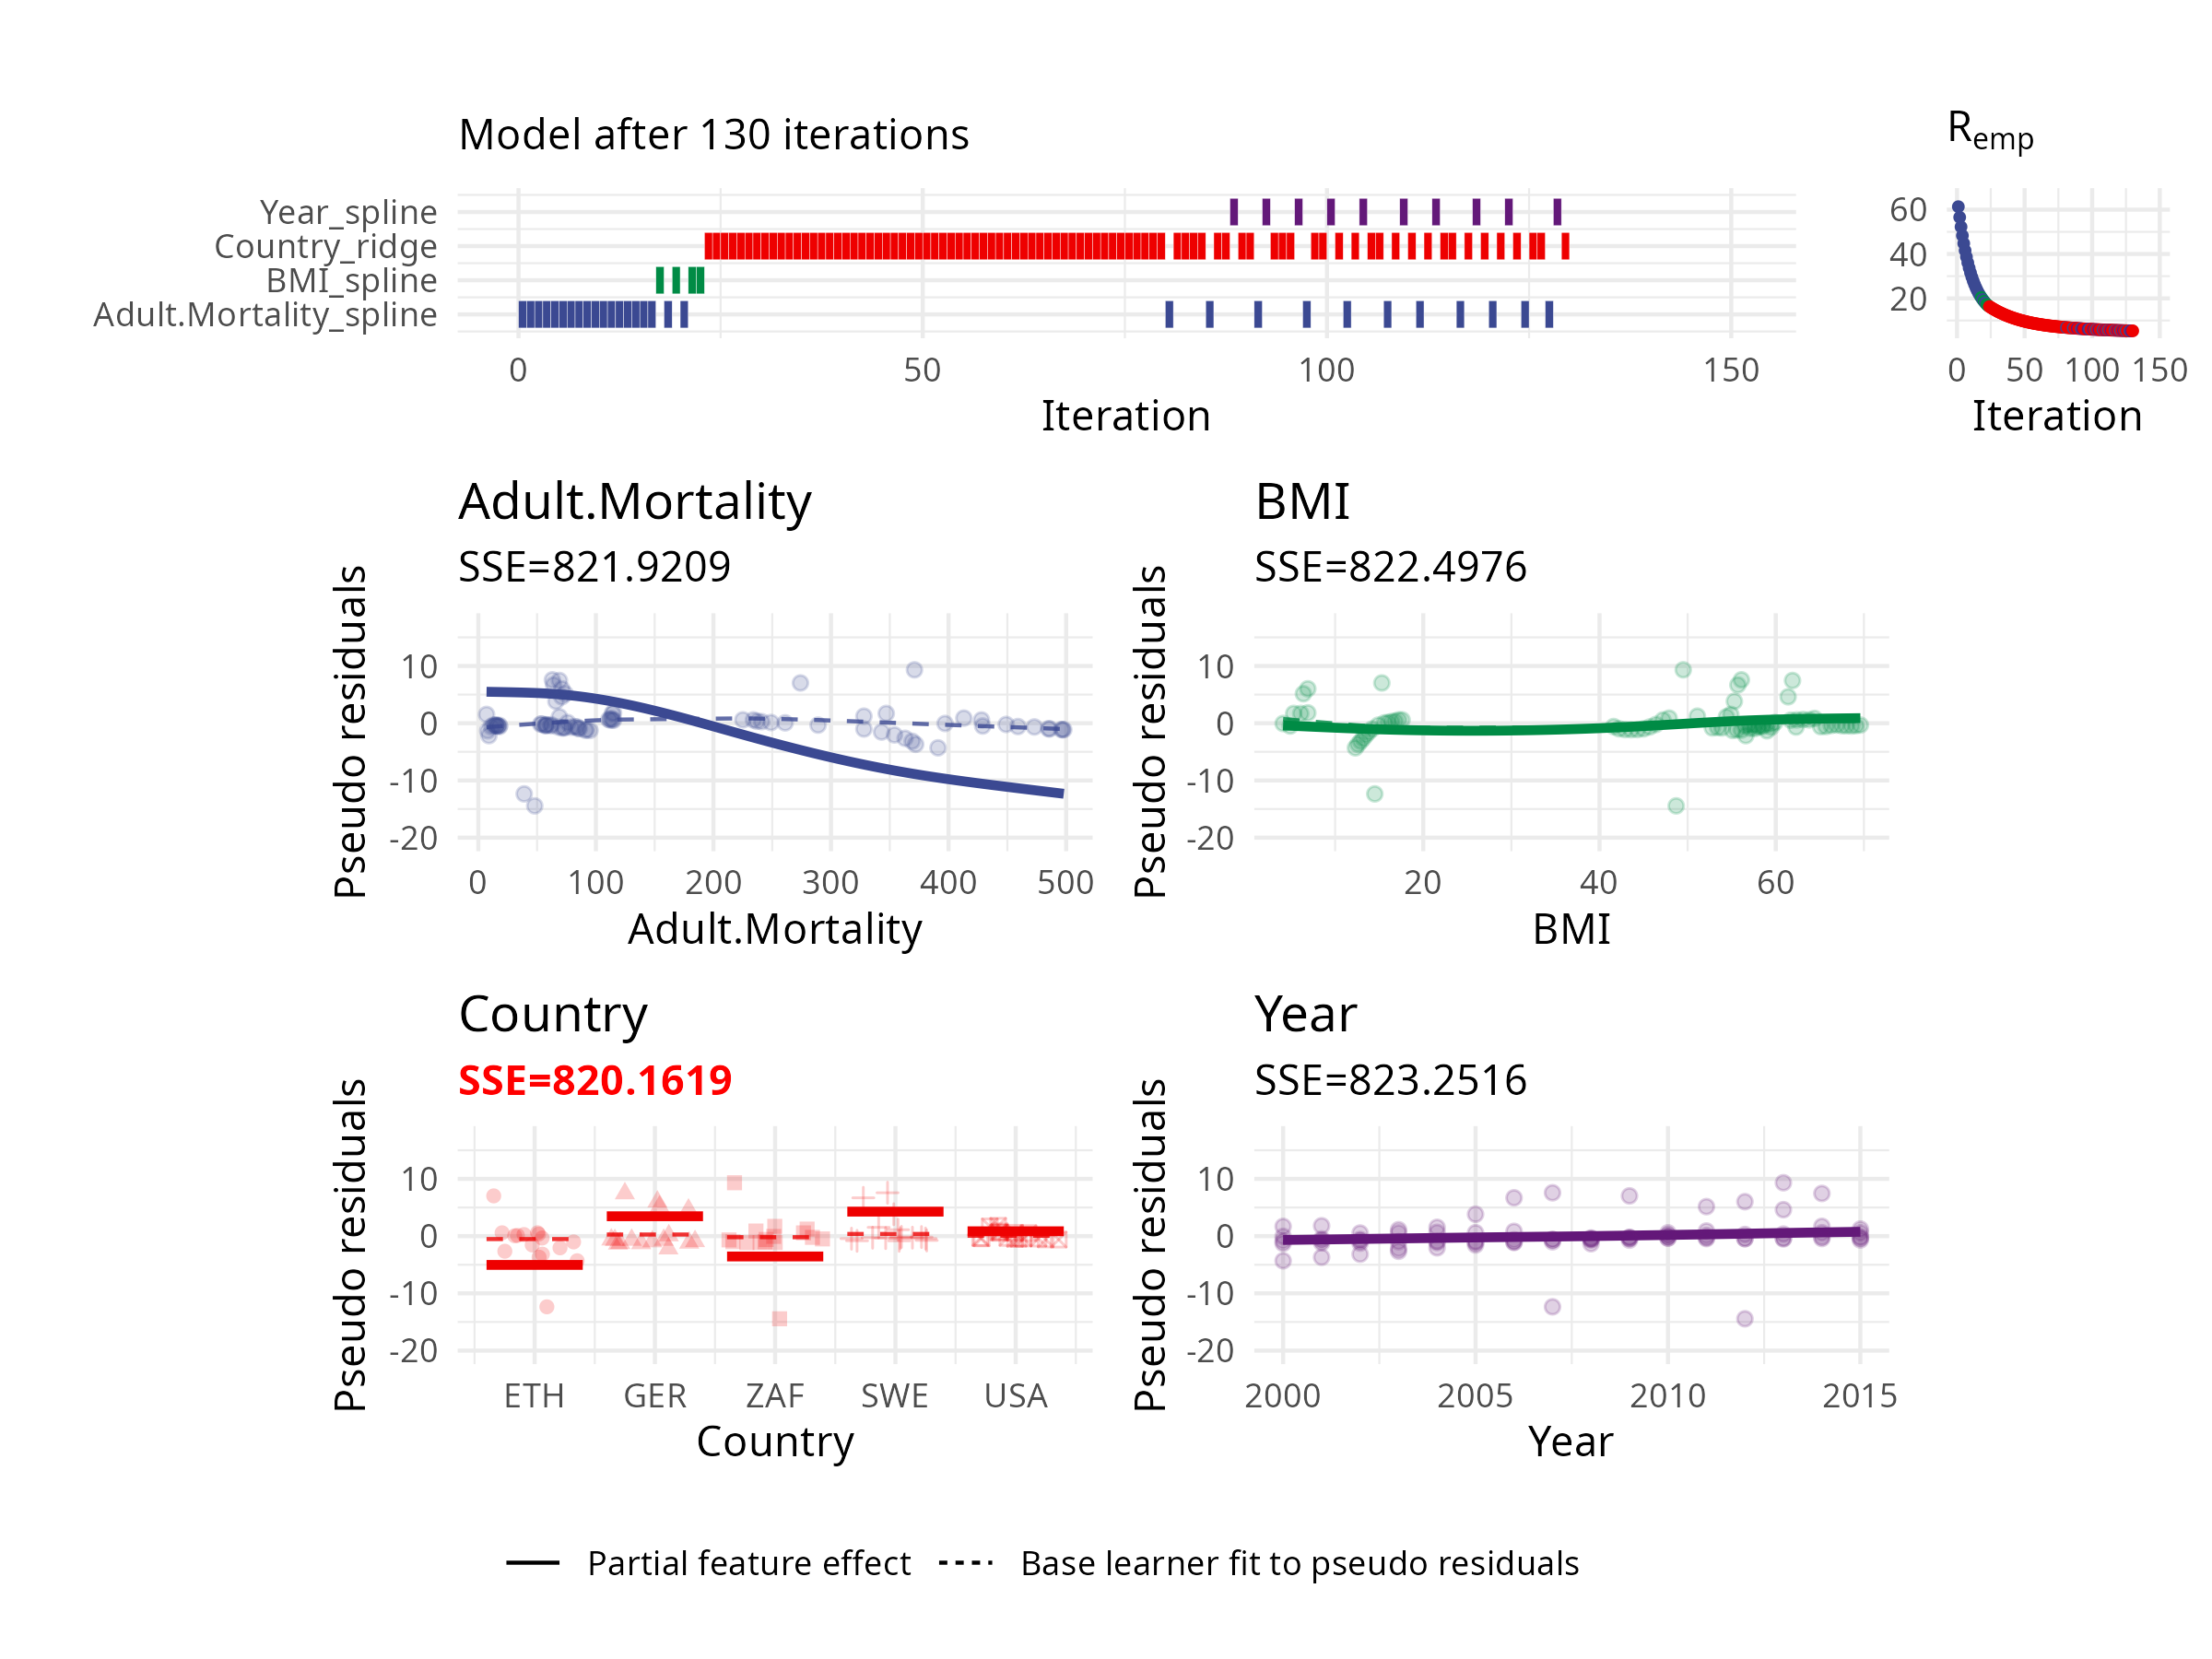
\includegraphics[width=\textwidth]{figure/cwb-anim-nl/fig-iter-0130.png}
	\end{figure}
	\addtocounter{framenumber}{-1}
\end{frame}


\begin{frame}{Example: Life expectancy (nonlinear)}
	\begin{figure}
		\centering
		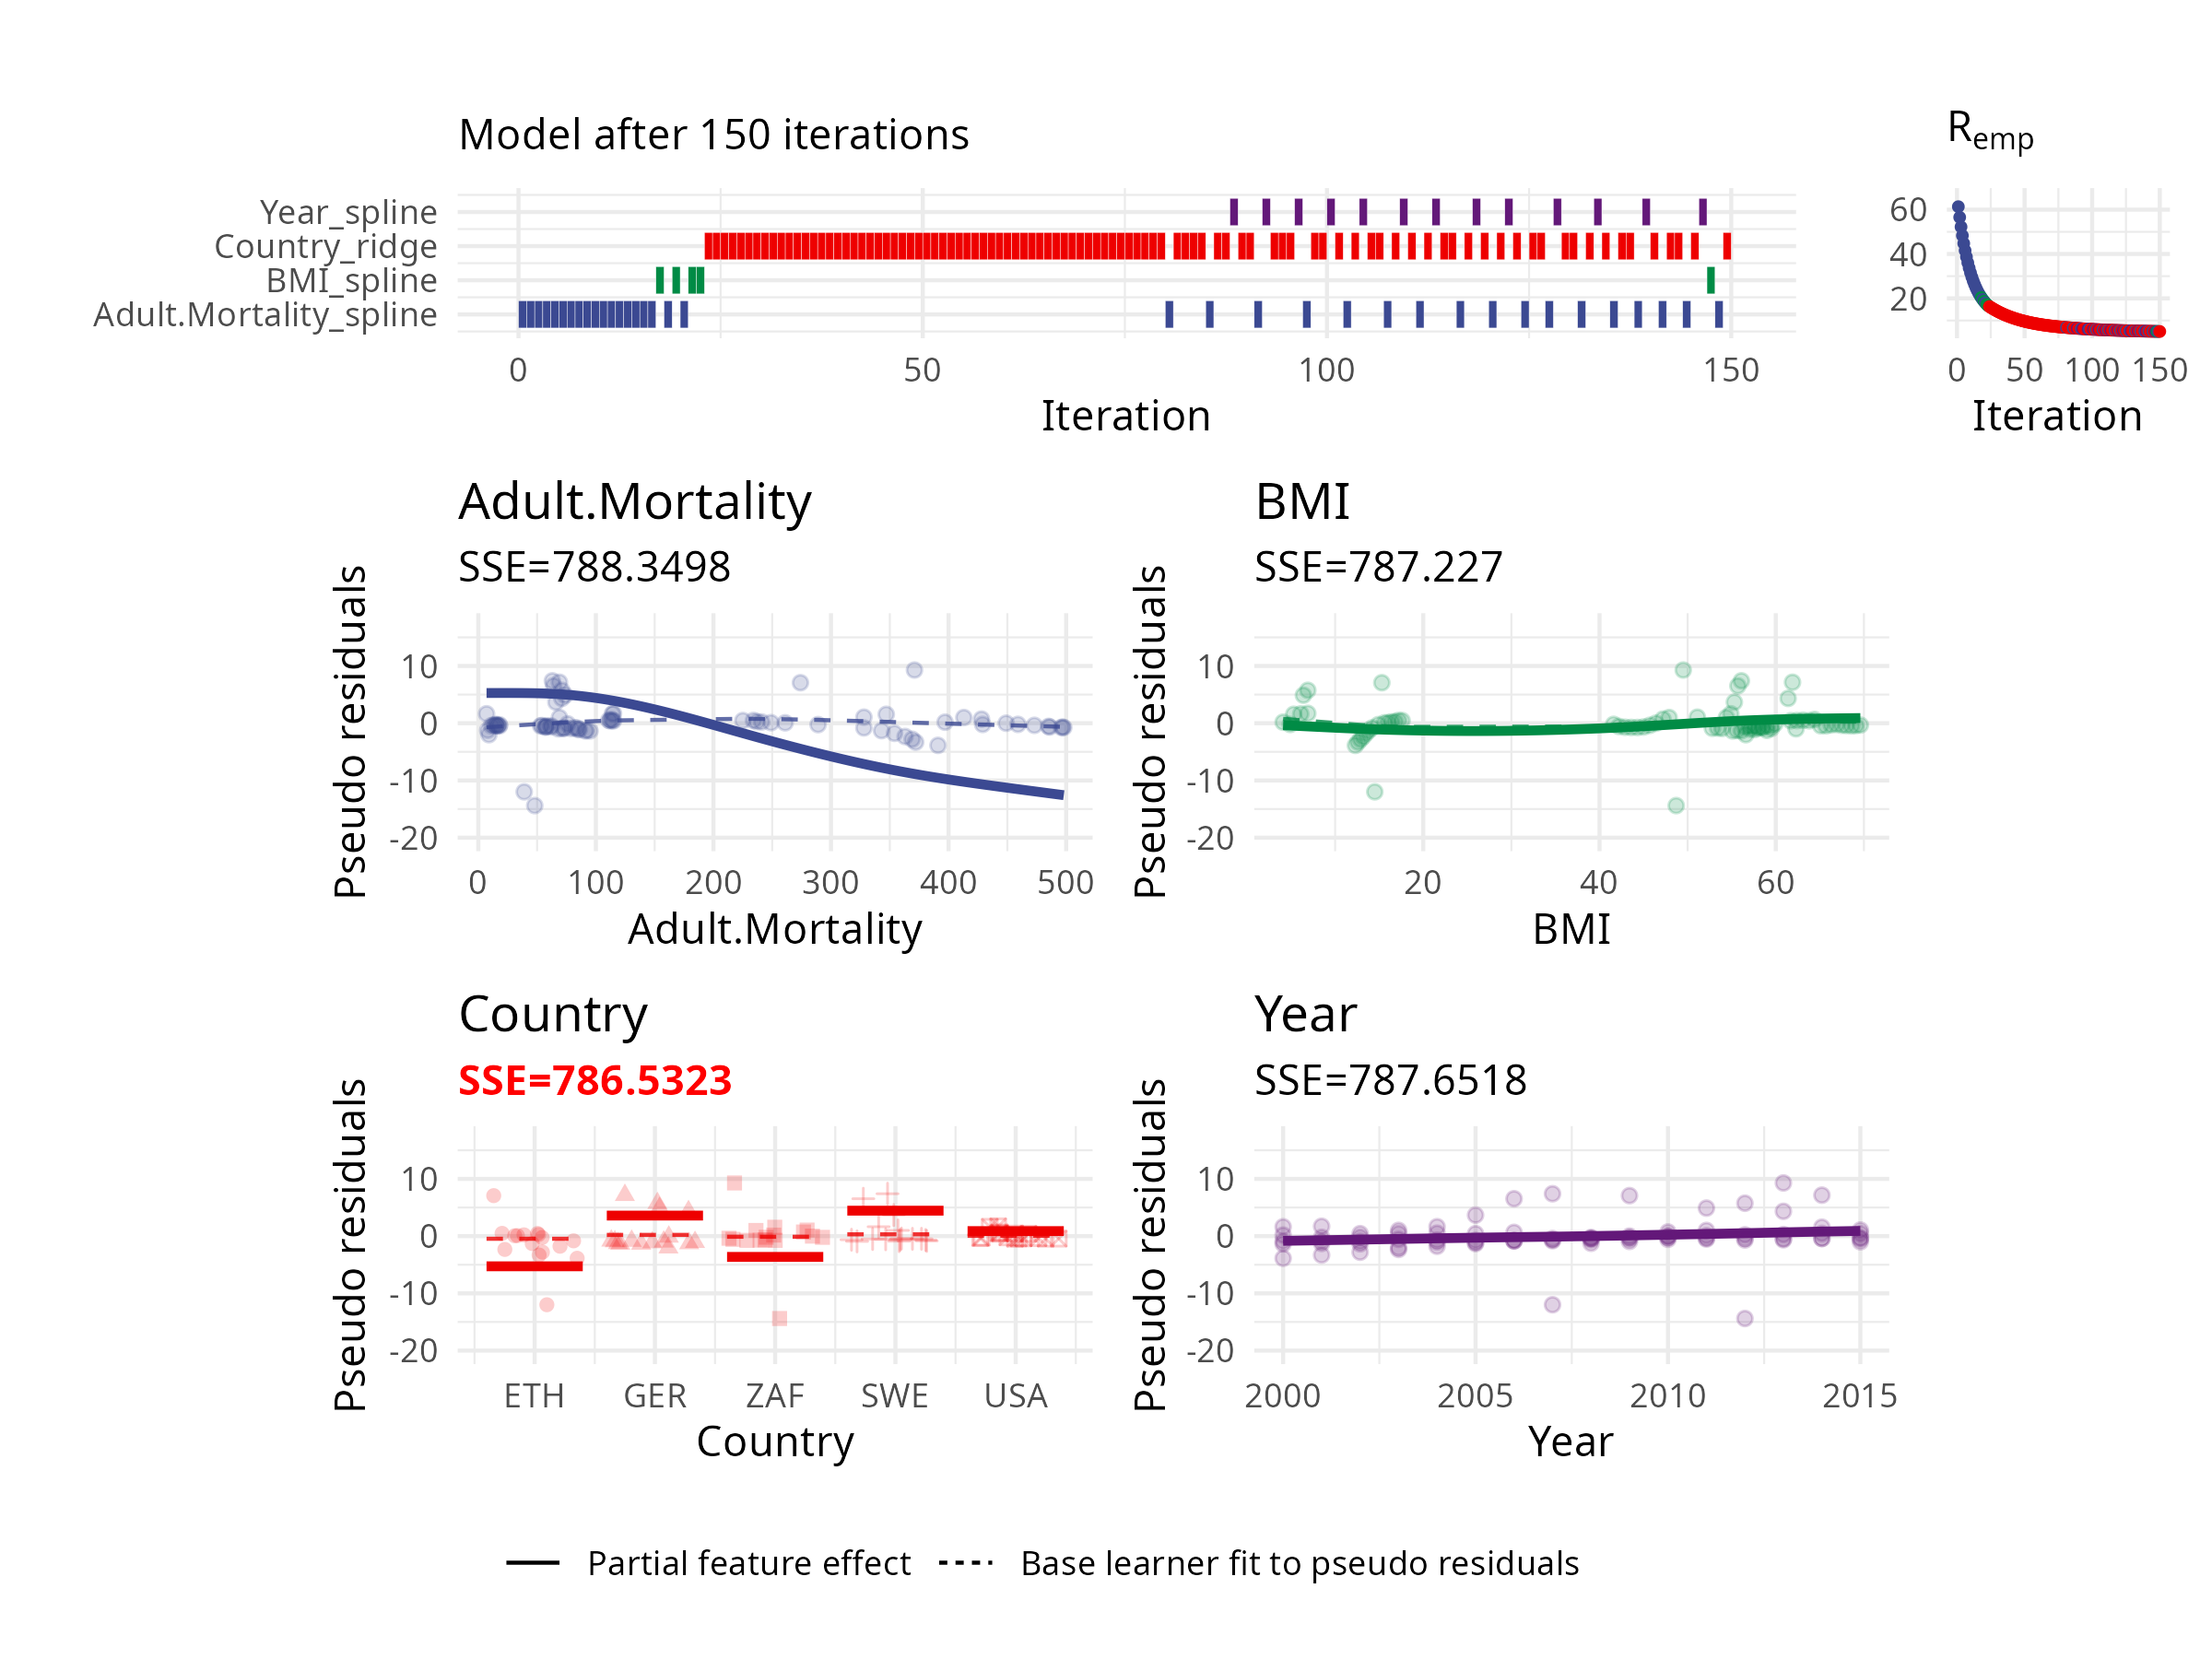
\includegraphics[width=\textwidth]{figure/cwb-anim-nl/fig-iter-0150.png}
	\end{figure}
	\addtocounter{framenumber}{-1}
\end{frame}



%\begin{vbframe}{boston housing: continued}
%
%\begin{itemize}
%  \small
%  \item This time we offer our model both
%  linear and nonlinear ($P$-spline) base learners (again, with intercept) for
%  the 13 features.
%  \item By iteration 100, the model has selected 8 out of the resulting 26 base
%  learners and consistently picked the nonlinear option.
%  We can trace how these spline predictors evolve over the iterations:
%\end{itemize}
%
%\vfill
%
%\begin{center}
%% \includegraphics[width=0.6\textwidth]{figure_man/spam-example.png}
%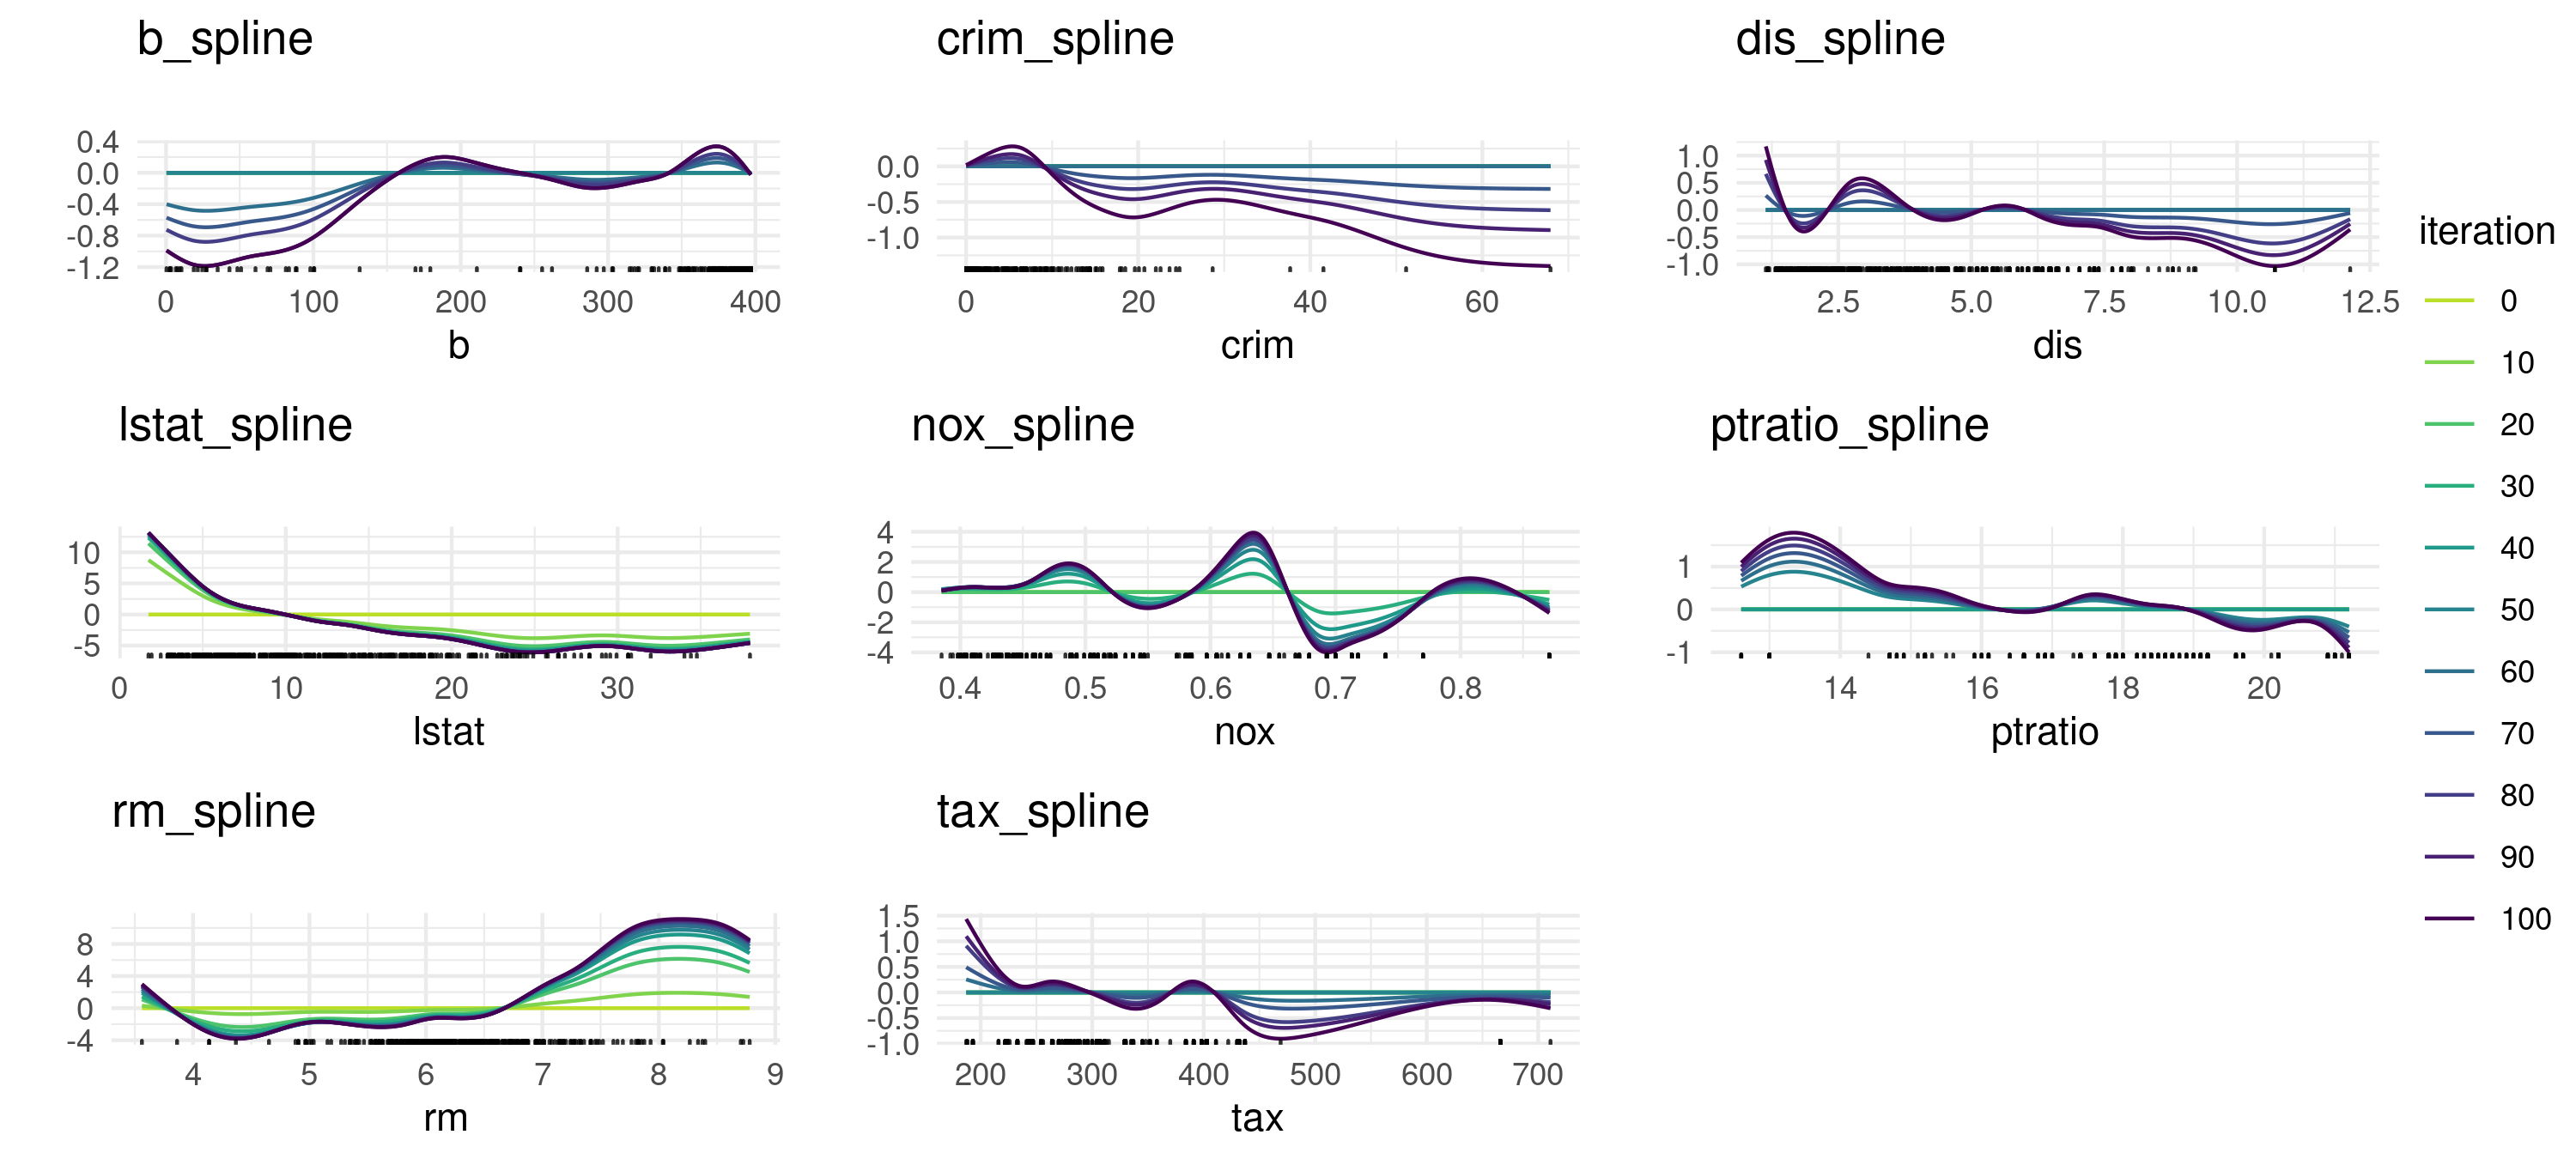
\includegraphics[width = \textwidth]{figure/compboost-illustration-3.png}
%\end{center}

% Unfortunately it's rather ugly to write down the decomposition

% <<spam-formula, eval = FALSE, echo = TRUE>>=
% formula <-
%   spam ~ bols(word_freq_make) + bbs(word_freq_make, df = 2, center = TRUE) +
%     bols(word_freq_address) + bbs(word_freq_address, df = 2, center = TRUE) +
%     bols(word_freq_all) + bbs(word_freq_all, df = 2, center = TRUE) +
% #  ...
% mboost(formula, data = spam, family = Binomial(), control = boost_control(mstop = 100))
% @
%
%\end{vbframe}

% ------------------------------------------------------------------------------

\begin{vbframe}{Nonlinear effect decomposition}

Even when allowing for more complexity we typically want to keep solutions as
simple as possible.

\lz

Kneib~et~al. (2009) proposed a decomposition of each base learner into a
constant, a linear and a nonlinear part.
The boosting algorithm will automatically decide which feature to include --
linear, nonlinear, or none at all:

\vspace{-0.7cm}

\begin{align*}
b_j(x_j, \thetam) & = b_{j, \text{const}}(x_j, \thetam) + b_{j, \text{lin}}
(x_j, \thetam) + b_{j, \text{nonlin}}(x_j, \thetam)\\
 & = \theta^{[m]}_\text{j,const} + x_j \cdot \theta^{[m]}_{j, \text{lin}} +
 s_j(x_j, \thetam_{j,\text{nonlin}}),
\end{align*}

\small
where
\begin{itemize}
  \small
  \item $\theta_\text{j,const}$ is the intercept of feature $j$,
  \item $x_j \cdot \theta^{[m]}_{j, \text{lin}}$ is a feature-specific linear
  base learner, and
  \item $s_j(x_j, \thetam_{j,\text{nonlin}})$ is a (centered) nonlinear base
  learner capturing deviation from the linear effect (see next slide).
\end{itemize}

\framebreak

\begin{itemize}
    \item 
        Suppose a base learner $b_{j,\text{nonlin}}\in\mathcal{B}_{j,\text{nonlin}}$ (a spline base learner) with design matrix $\bm{Z}_{j,\text{nonlin}}\in\R^{n\times d_{j,\text{nonlin}}}$ and a linear base learner $b_{j,\text{lin}}\in\mathcal{B}_{j,\text{lin}}$ with design matrix $\bm{Z}_{j,\text{lin}}\in\R^{n\times d_{j,\text{nonlin}}}$.

    \item
        Often, $\mathcal{B}_{j,\text{lin}} \subseteq \mathcal{B}_{j,\text{nonlin}}$ and hence $b_{j,\text{lin}}$ is overlayed by $b_{j,\text{nonlin}}$ and not selected during the fitting.

     \item
        Subtracting $b_{j,\text{lin}}$ from $b_{j,\text{nnnlin}}$ to obtain a centered nonlinear base learner $b_{j,\text{nnonlin}^c}$ means to transform $\bm{Z}_{j,nonlin}$ so that the $span(\bm{Z}_{j,lin})$ is not included in $span(\bm{Z}_{j,nonlin})$. 

    \item 
        Practically, this means that $b_{j,\text{nonlin}^c}\notin \mathcal{B}_{j,\text{lin}}$ and hence cannot model any linear effect.

    \item
        The centering is done by computing the QR decomposition of $\bm{A} = \bm{Z}_{j,nonlin}^T \bm{Z}_{j,lin}$.

    \item 
        The first $k$ columns of the $\bm{Q}$ matrix from the QR decomposition form an orthonormal basis for the span of the first $k$ columns of $\bm{A}$.

    \item 
        Hence $\bm{Q}^\ast$, which is $\bm{Q}$ without the first $d_{j,\text{lin}}$ columns rotates $\bm{Z}_{j,nonlin}$ to $\bm{Z}_{j,nonlin^c} = \bm{Q}^\ast\bm{Z}_{j,nonlin}\in\R^{n\times d_{j,nonlin} - d_{j,lin}}$ which defines $b_{j,\text{nnonlin}^c}$
\end{itemize}

\end{vbframe}

\begin{vbframe}{Example: Nonlinear effect decomposition}

\begin{itemize}
    \item 
        Suppose $n = 100$ uniformly distributed $x$ values between $0$ and $10$.

    \item 
        The response $y = 2\sin(x) + 2x$ has a nonlinear and linear component.

    \item
        We apply CWB with $M = 500$ to $\{(\xi, \yi) | i = 1, \dots, n\}$ with:
        \begin{itemize}
            \item One model with $\mathcal{B} = \{b_{j,\text{lin}}, b_{j,\text{nonlin}}\}$
            \item One model with $\mathcal{B} = \{b_{j,\text{lin}}, b_{j,\text{nonlin}^c}\}$
        \end{itemize}
\end{itemize}

% Create figures with: rsrc/fig-centered-bl.R
\begin{figure}
    \centering
    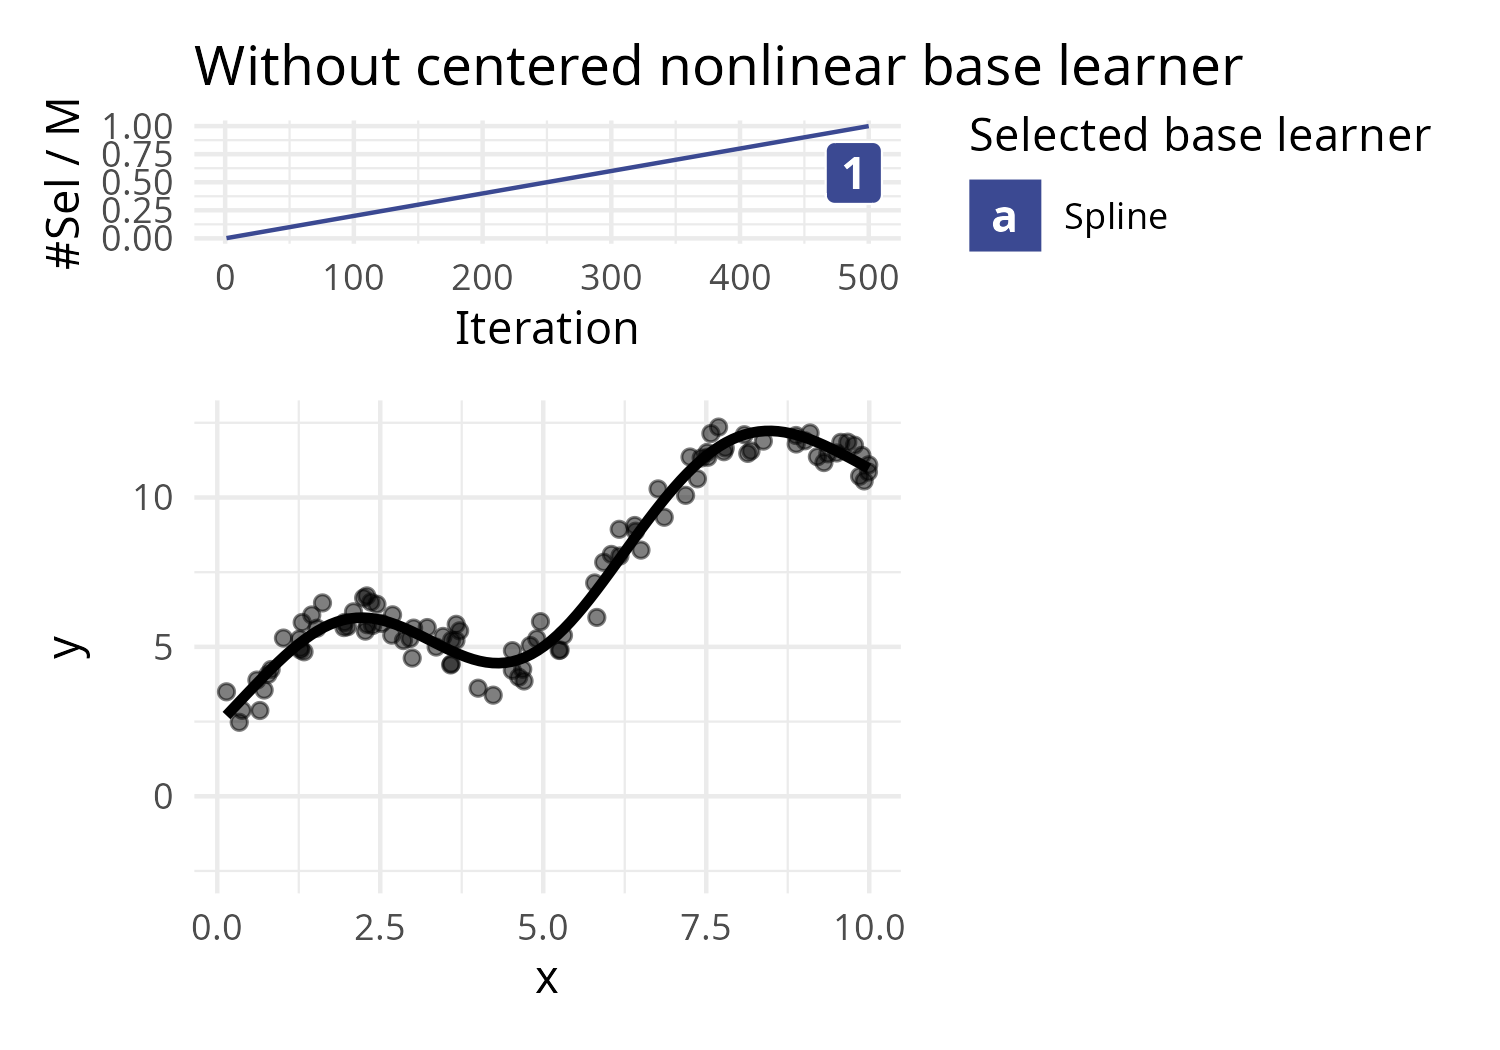
\includegraphics[width=0.45\textwidth]{figure/fig-decomp1.png}
    \hfill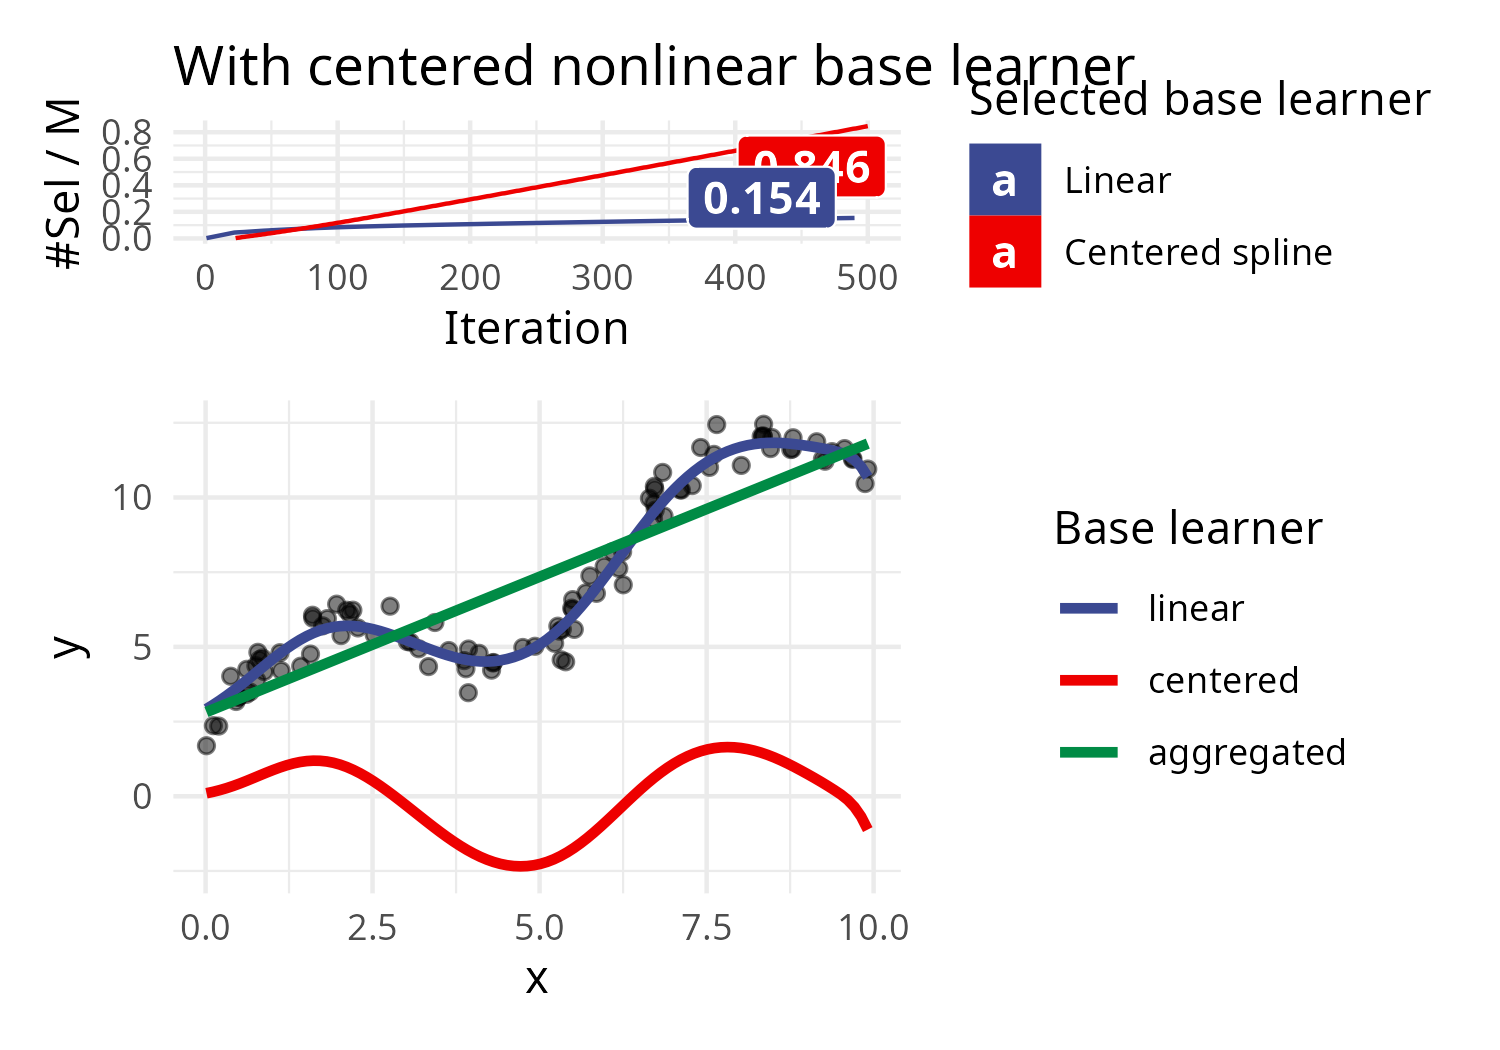
\includegraphics[width=0.45\textwidth]{figure/fig-decomp2.png}
\end{figure}

\end{vbframe}


% ------------------------------------------------------------------------------

\begin{vbframe}{Fair Base Learner Selection}

\begin{itemize}

  \item
    Using splines and linear base learners in CWB will favor
    the more complex spline base learner over the linear base learner.

  \item
    This makes it harder to achieve the desired behavior of the base learner
    decomposition as explained previously.

  \item
    To conduct a fair base learner selection we set the degrees of freedom of all base learners equal.

  \item
    The idea is to set the regularization/penalty term of a single learner in a manner that their complexity is treated equally.

\end{itemize}

\framebreak

% ------------------------------------------------------------------------------

Especially for linear models and GAMs it is possible to transform the degrees of freedom into a corresponding penalty term.

\textcolor{red}{@BB nochmal nachlesen}

\begin{itemize}

  \item
    Parameters of the base learners are estimated via:
    $$
    \thetam_j = \left(\mathbf{Z}_j^T \mathbf{Z}_j + \lambda_j \mathbf{K}_j
    \right)^{-1}\mathbf{Z}_j^T \rmm\,,
    $$
    with $\mathbf{Z}_j$ the design matrix of the $j$-th base learner,
    $\lambda_j$ the penalty term, and $\mathbf{K}_j$ the penalty matrix.

  \item
    Having that kind of model, we use the hat matrix
    $\mathbf{S}_j = \mathbf{Z}_j\left(\mathbf{Z}_j^T \mathbf{Z}_j +
    \lambda_j \mathbf{K}_j\right)^{-1}\mathbf{Z}_j^T$ to define the degrees of
    freedom:
    $$
    \operatorname{df}(\lambda_j) = \trace\left(2\mathbf{S}_j - \mathbf{S}_j^T
    \mathbf{S}_j\right).
    $$
    \textbf{Note:} With $\lambda_j = 0$, $\mathbf{S}_j$ is the projection matrix
    into the target space with
    $\trace(\mathbf{S}_j) = \operatorname{rank}(\Xmat)$, which corresponds to
    the number of parameters in the model.

\end{itemize}

\framebreak

% ------------------------------------------------------------------------------

It is possible to calculate $\lambda_j$ by applying the Demmler-Reinsch
orthogonalization (see
\href{https://www.tandfonline.com/doi/abs/10.1198/jcgs.2011.09220}
{Hofer et al. (2011)}).

% (see Hofer et. al. (2011).\textit{\enquote{A framework for unbiased model selection based on boosting.}}).

Consider the following example of a GAM using splines with 24 parameters:

\begin{itemize}

  \item
    Setting $\operatorname{df} = 24$ gives $B$-splines with $\lambda_j = 0$.

  \item
    Setting $\operatorname{df} = 4$ gives $P$-splines with $\lambda_j = 418$.

  \item
    Setting $\operatorname{df} = 2$ gives $P$-splines with $\lambda_j = 42751174892$.

\end{itemize}

\begin{center}
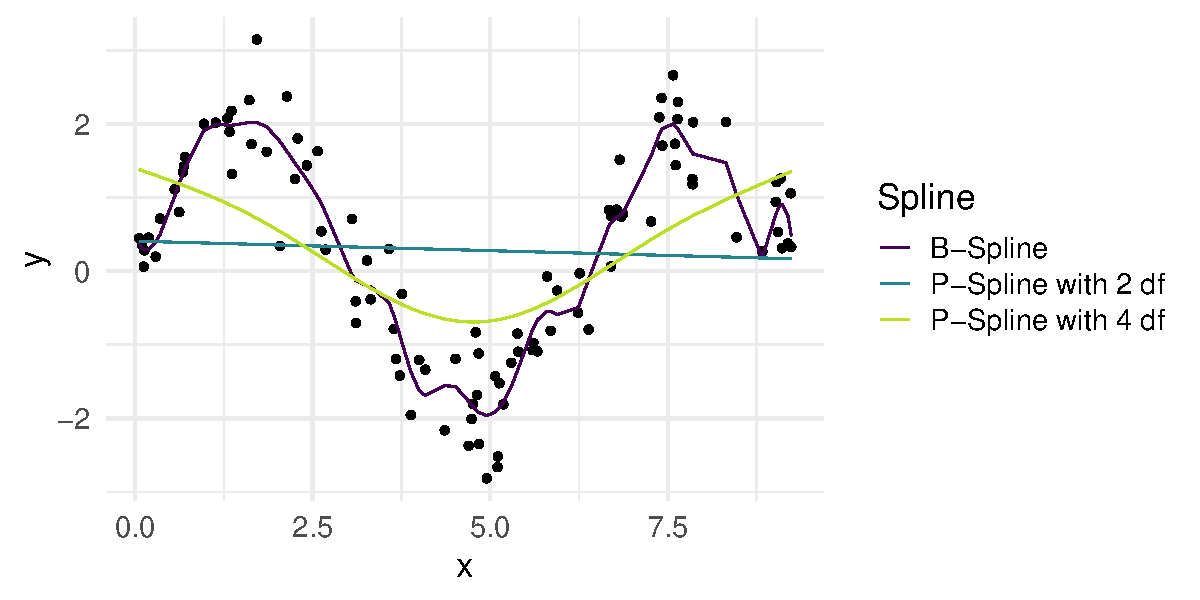
\includegraphics[width=0.7\textwidth]{figure_man/df_to_lambda.pdf}
\end{center}

\end{vbframe}

\begin{vbframe}{Available base learners}

There is a large amount of possible base learners, e.g.:

\begin{itemize}
  \item Linear effects and interactions (with or without intercept)
  \item Uni- or multivariate splines and tensor product splines
  \item Trees
  \item Random effects and Markov random fields
  \item Effects of functional covariates
  \item ...
\end{itemize}

\lz

In combination with the flexible choice of loss functions, this allows boosting to fit  a huge number of different statistical models with the same algorithm. Recent extensions include GAMLSS-models, where multiple additive predictors are boosted to model different distribution parameters (e.g., conditional mean and variance for a Gaussian model).

\end{vbframe}
% ------------------------------------------------------------------------------
\begin{vbframe}{Partial Dependence Plots (PDP)}

If we use single features in base learners, we think of each base learner as a wrapper around a feature which represents the effect of that feature on the target variable. Base learners can be selected more than once (with varying parameter estimates), signaling that this feature is more important.\\
E.g. let $j \in \{ 1,2,3 \}$, the first three iterations might look as follows
\begin{align*}
m = 1: \quad & \hat{f}^{[1]}(\xv) = \hat{f}^{[0]} + \alpha \textcolor{blue}{\hat{b}_2(x_2, \hat{\theta}^{[1]})}\\
m = 2: \quad & \hat{f}^{[2]}(\xv) = \hat{f}^{[1]} + \alpha  \textcolor{orange}{\hat{b}_3(x_3, \hat{\theta}^{[2]})}\\
m = 3: \quad & \hat{f}^{[3]}(\xv) = \hat{f}^{[2]} + \alpha \textcolor{blue}{\hat{b}_2(x_2, \hat{\theta}^{[3]})}
\end{align*}

Due to linearity, $\hat{b}_2$ base learners can be aggregated:
$$
\hat{f}^{[3]}(\xv) = \hat{f}^{[0]} + \alpha (\textcolor{blue}{\hat{b}_2(x_2, \hat{\theta}^{[1]} + \hat{\theta}^{[3]})} + \textcolor{orange}{\hat{b}_3(x_3, \hat{\theta}^{[2]})})
$$

Which is equivalent to:
$\hat{f}^{[3]}(\xv) = \hat{f}_0 + \textcolor{blue}{\hat{f}_2(x_2)} + \textcolor{orange}{\hat{f}_3(x_3)}$.\\
Hence, $\hat{f}$ can be decomposed into the marginal feature effects (PDPs).



\end{vbframe}




\begin{vbframe}{Feature importance}
\begin{itemize}
  \item We can further exploit the additive structure of the boosted ensemble to
  compute measures of \textbf{variable importance}.
  \item To this end, we simply sum for each feature $x_j$ the improvements in
  empirical risk achieved over all iterations until
  $1 < m_{\text{stop}} \leq M$:
  % \begin{align*}
    $$VI_j = \sum_{m = 1}^{m_{\text{stop}}} \left( \riske \left(
    \fmd(\xv) \right) - \riske \left(\fm(\xv)
    \right) \right) \cdot \I_{[j \in j^{[m]})]},$$
  % \end{align*}
\end{itemize}

\end{vbframe}

% \begin{vbframe}{Available base learners}
%
% There is a large amount of possible base learners, e.g.:
%
% \begin{itemize}
%   \item Linear effects and interactions (with or without intercept)
%   \item Uni- or multivariate splines and tensor product splines
%   \item Trees
%   \item Random effects and Markov random fields
%   \item Effects of functional covariates
%   \item ...
% \end{itemize}
%
% \lz
%
% In combination with the flexible choice of loss functions, this allows boosting to fit  a huge number of different statistical models with the same algorithm. Recent extensions include GAMLSS-models, where multiple additive predictors are boosted to model different distribution parameters (e.g., conditional mean and variance for a Gaussian model).
%
% \end{vbframe}

% ------------------------------------------------------------------------------

% \begin{vbframe}{RF vs AdaBoost vs GBM vs Blackboost}

% Again the Spirals data from mlbench. Blackboost: mboost with regression trees as base learners
% \end{vbframe}

\begin{vbframe}{Take-home message}

\begin{itemize}
  \item Componentwise gradient boosting is the statistical re-interpretation of
  gradient boosting.
  \item We can fit a large number of statistical models, even in high dimensions
  ($p \gg n$).
  \item A drawback compared to statistical models is that we do not get valid
  inference for coefficients $\rightarrow$ post-selection inference.
  % This can be (partially) solved by bootstrap inference or related methods.
  \item In most cases, gradient boosting with tree will dominate componentwise
  boosting in terms of performance due to its inherent ability to include
  higher-order interaction terms.
  % In most cases, componentwise gradient boosting will have worse
  % predictive performance than gradient boosting with trees. This is often
  % because additive base learner motivated by regression models (LM, GLM, GAM)
  % usually do not include higher-order interaction terms.
\end{itemize}

\end{vbframe}

% ------------------------------------------------------------------------------

\endlecture
\end{document}
